\documentclass{article}
\usepackage[utf8]{inputenc}
\usepackage{csquotes}
\usepackage[english]{babel}
\usepackage{appendix}
\usepackage{multicol}
\usepackage{titlesec}
\usepackage[nottoc]{tocbibind}
\usepackage{listings}
\usepackage{multicol}
\usepackage{titling}
\usepackage{graphicx}
\usepackage{tabularx}
\usepackage{float}
\usepackage{arydshln}
\usepackage{soul}
\usepackage{amsmath}
\usepackage{enumitem}
\usepackage{natbib}
\usepackage{titling}

\setcounter{tocdepth}{4}
\setcounter{secnumdepth}{4}

\titleformat{\paragraph}
{\normalfont\normalsize\bfseries}{\theparagraph}{1em}{}
\titlespacing*{\paragraph}
{0pt}{3.25ex plus 1ex minus .2ex}{1.5ex plus .2ex}



\newcommand{\subtitle}[1]{%
\posttitle{%
\par\end{center}
\begin{center}\large\textit{#1}\end{center}
\vskip0.5em}%
}
\bibliographystyle{agsm}


\title{What is required by software platforms in order to give a good developer experience?}
\subtitle{A Case Study in Qlik Core's Developer Experience}
\author{Christoffer MacFie}
\date{January 2019}

\begin{document}
\maketitle
\newpage
\newpage
\begin{abstract}
Lorem ipsum dolor sit amet, consectetur adipiscing elit, sed do eiusmod tempor incididunt ut labore et dolore magna aliqua. Ut enim ad minim veniam, quis nostrud exercitation ullamco laboris nisi ut aliquip ex ea commodo consequat. Duis aute irure dolor in reprehenderit in voluptate velit esse cillum dolore eu fugiat nulla pariatur. Excepteur sint occaecat cupidatat non proident, sunt in culpa qui officia deserunt mollit anim id est laborum.
\end{abstract}
\textbf{Keywords: keyword1, keyword2, keyword3}
\newpage
\Large{\textbf{Aknowledgements}} \\
\normalsize
More text here...
\newpage
\tableofcontents
\newpage

\section{Background and Purpose}

Text here introducing what this paper will be about

\subsection{What is User Experience?}

User Experience (UX) is the collective term of many disciplines merged
into one that evaluates the overall experience delivered to a user of a
system, product or service. The coining of the term is often attributed to \cite{norman}, who has who has a background in the fields of cognitive science and usability engineering. There isn't one definitive of what UX is. They one who created the term, Norman, defines UX as:
\begin{quote}
"All aspects of the end-user’s interaction with the company, its services, and its products. The first requirement for an exemplary user experience is to meet the exact needs of the customer, without fuss or bother. Next comes simplicity and elegance that produce products that are a joy to own, a joy to use. True user experience goes far beyond giving customers what they say they want, or providing checklist features. In order to achieve high-quality user experience in a company’s offerings there must be a seamless merging of the services of multiple disciplines, including engineering, marketing, graphical and industrial design, and interface design."
\end{quote}
User Experience has since it's emergence in the 1990s gotten its own ISO-standard: ISO-9241-210. It is defined by \cite{iso9241}, part
of "Ergonomics of human system interactions", as \begin{quote}
"A person's perceptions and responses that result from the use or anticipated use of a product, system or service"
\end{quote}
World Wide Web Consortium (W3C) is the main international standards organization for the World Wide Web. \cite{w3c} defines it as following:
\begin{quote}
"A set of material rendered by a user agent which may be perceived by a user and with which interaction may be possible."
\end{quote}
One common denominator is that UX is related to how something is \textit{perceived}. It can therefor be considered a somewhat
subjective quality of a product, system or service. Because of this it can be hard to measure with exact numbers. \cite{iso9241} has a four-part process how to evaluate a system or service. The process can be seen in figure \ref{fig:iso9241}. It's an iterative process, and depending if the design solution  meets the user requirements or not, an earlier phase in the process needs to be revisted.
\begin{figure}[H]
\centering
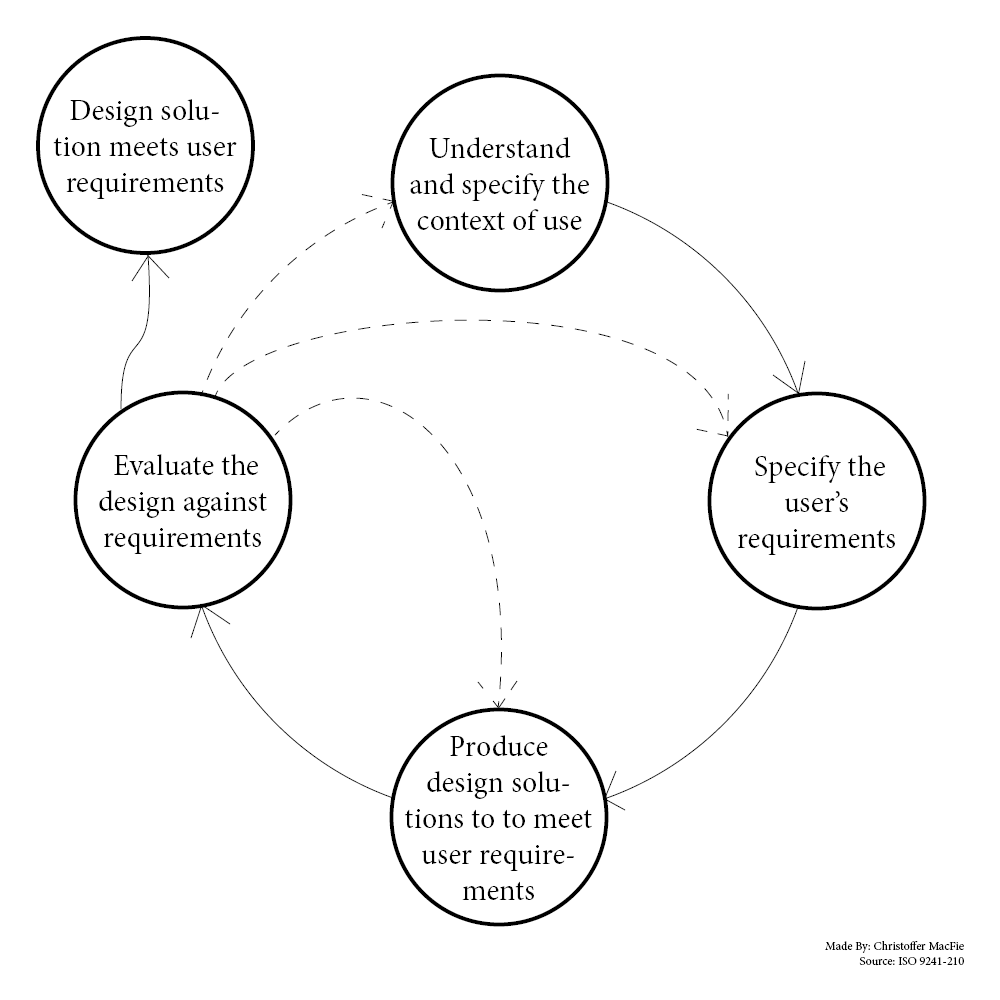
\includegraphics[width=\linewidth]{iso9241-210.png}
\caption{The UX evaluation process as defined by ISO 9241-210}
\label{fig:iso9241}
\end{figure}
\subsection{What is Developer Experience?}

Developer Experience, or DX, is similar to the more well known User
Experience (UX), but with the user being a software developer. Developer Experience has yet to be defined by any standards organization. There is also limited peer-reviewed academic research around the subject. That doesn't however mean that there isn't articles about it. DX is
defined by \cite{jarman} as
\begin{displayquote}
"The experience developers have when they use your product, be it
client libraries, SDKs, frameworks, open source code, tools, API,
technology or service."
\end{displayquote}
\cite{dhide} has written an article around how he and a team of developer tries to define DX. As he puts it:
\begin{quote}
"Developer Experience (DX) is inspired by the User Experience practice and sees developers as a special case of users. Developer Experience Design is the practice of understanding how developers get their work done, and optimizing that experience."
\end{quote}
In this paper we will use the following definition, inspired by UX-defintions:
\begin{quote}
"Developer Experience is the perceived feelings and thoughts of a developer, generated by an interaction with a software or service that is meant to be used by a software developer"
\end{quote}
\subsection{How Can One Define What Is 'Good DX'?}
There are many potential factors for defining what constitutes 'Good'
DX. The website \cite{everydeveloper} has developed a \textit{DX Index} from
1-10, where they consider four factors:

\begin{enumerate}
\item Are the libraries available in popular languages?
\item How prominent, in-depth are the starting guides?
\item Are the solutions self-serving, without need of demos or 'call us'?
\item Is the pricing clearly stated?
\end{enumerate}
\cite{jarman} has other factors for he uses to evaluate
if something gives a good DX. He for example puts emphasis on
communication between the product provider and the developer. The dialog
between the product provider and the community needs to be authentic,
open and honest in order the give a good developer experience, according
to Jarman.
\\ \\
\cite{dhide} workshop generated a list of things that they think should be considered when designing software or services with good DX. They're key aspects are simplicity, usability, innovation and "delightfulness". They put emphasis on "Less is more", stating that "Any element that isn't helping the user achieve their goal is working against them". Some other things they say is important are "Always keep the target users in mind as the product is designed", "Know what type of problem you’re solving" and "Use concepts familiar to the user rather than system-oriented terms".
\\ \\
It has been researched by \cite{unhappy} what makes a developer
happy and unhappy, and they found several indicators, both
internal- and external factors. They pointed both to internal factors, the developers own well-being. These factors were things like stress, fatigue, low motivation, etc. They also pointed to external factors. These were things like low productivity, delays, broken flow, and more. According to their findings, low productivity is the most common cause of unhappiness among developers. This is something that may be improved by software giving better DX. This research shows that there is a clear need for good DX.
\subsection{What is Qlik Core?}
Qlik Core (QC) is, as described on the official website, "an analytics
development platform built around Qlik Associative Engine and
Qlik-authored open source libraries".\cite{qlikwebsite} The
platform consists of several components, with it's central part being
the engine. The platform also provides 'Mira', a software to generate
insights about the data. Furthermore, it provides the two javascript
libraries 'Halyard' and 'Enigma'. Halyard helps the user to easily load
in data into the engine. Enigma helps the user communicate with the
engine.

More text here...


\subsection{Standardisation}
International Organisation for Standardization (ISO) has yet to present a
standard for developer experience. There are however other standards from ISO
that are interesting to have a look at. One is \textit{ISO 9126 Software engineering - Product Quality}.
One part of the ISO-standard concerns quality. This part of the ISO standardizes how to measure the quality of software.
It has six different characteristics: functionality, reliability, usability, efficiency, maintainability and
portability. Each of these characteristics have sub-characteristics. The definition of each
characteristic is listed, and their sub-characteristics, is in table \ref{tabl:standard1} and table \ref{tabl:standard2}


\begin{table}[H]
\centering
\begin{tabularx}{\columnwidth}{|l|l|X|}
\hline

\multicolumn{3}{c}{\textbf{Functionality}} \\ \hline
F1  &   Suitability &The capability of the software product to provide an appropriate set of
functions to specified tasks and objectives \\ \hline
F2  &   Accurateness &  The cap... / / ... to provide the right or agreed results or effects with the needed
degree of precision \\ \hline
F3  &   Interoperability& The cap... / / ... to interact with one or more specified systems \\ \hline
F4  &   Security& The cap... / / ... to protect information and data so that unauthorised persons or systems
cannot read or modify them and authorised persons or systems are not denied access to them \\ \hline

\multicolumn{3}{c}{\textbf{Reliability}} \\ \hline
R1  & Maturity    & The cap... / / ... to avoid failure as a result of faults in the software \\
\hline
R2  &   Fault tolerance & The cap... / / ... to maintain a specified level of performance in cases of the
software faults or of infringement of its specified interface \\ \hline
R3  &   Recoverability  & The cap... / / ... to re-establish a specified level of performance and recover the
data directly affected in the case of a failure \\ \hline

\multicolumn{3}{c}{\textbf{Usability}} \\ \hline
U1  &   Understandability   &   The cap... / / ... to enable the user to understand whether the
software is suitable, and how it can be used for particular tasks and conditions of use \\ \hline
U2&Learnability & The cap... / / ... to enable the user to learn it application \\ \hline
U3&Operability & The cap... / / ... to operate and control it \\ \hline
U4&Attractiveness& The cap... / / ... to be attractive to the user [visually] \\ \hline

\multicolumn{3}{c}{\textbf{Efficiency}} \\ \hline
E1&Time Behaviour & The cap... / / ... to provide appropriate response and processing times and
throughput rates when performing its function, under stated conditions \\ \hline
E2&Resource Utilisation & The cap... / / ... to use appropriate amounts and types of resources when the software
performs its function under stated conditions \\ \hline
\end{tabularx}
\caption{Part 1: ISO-9216}
\label{tabl:standard1}
\end{table}

\begin{table}[H]
\centering
\begin{tabularx}{\columnwidth}{|l|l|X|}
\hline
\multicolumn{3}{c}{\textbf{Maintainability}} \\ \hline
M1&Analysability & The cap... / / ... to be diagnosed for deficiencies or causes of failures in the
software, or for the parts to be modified to be identified \\ \hline
M2&Changeability & The cap... / / ... to enable a specified modification to be implemented \\ \hline
M3&Stability & The cap... / / ... to avoid unexpected effects from modifications of the software \\ \hline
M4&Testability &The cap... / / ... to enable modified software to be validated \\ \hline

\multicolumn{3}{c}{\textbf{Portability}} \\ \hline
P1& Adaptability &The cap... / / ... to be adapted for different specified enviroments without applying
actions or means other than tose provided for this purpose for the software considered \\ \hline
P2&Installability& The cap... / / ... to be installed in a specified environment \\ \hline
P3&Co-existence &The cap... / / ... to co-exist with other independent software in a common enviroment sharing
common resources \\ \hline
P4&Replaceability &The cap... / / ... to be used in a place of another specified software product for the same
purpose in the same environment \\ \hline

\multicolumn{3}{c}{\textbf{All characteristics}} \\ \hline
AC&Compliance & The cap... / / ... to adhere to standards and conventions relating to the
characteristic \\ \hline
\end{tabularx}
\caption{Part 2: ISO-9216}
\label{tabl:standard2}
\end{table}
\subsection{Kinds of APIs}

Application Program Interfaces (APIs) are, simply put, a software that
lets one application interact with another application's inner data and
services. Applications are in need of an interface to interact with it's
inner parts to create, read, update and read (CRUD) as well as execute
commands. APIs provide this link between the two pieces of software that let's
them communicate.Because of APIs broad nature, there are many types of
APIs.

\subsubsection{Internal, Public and Partner APIs}
APIs have different level of openness, depending on who is going to access them. They are
usually divided into three groups: Internal APIs, Public APIs and Partner APIs. These
three groups are explained below.
\paragraph{Internal APIs}
Internal APIs are APIs that har meant to be used in production and
within an organisation or company. They are often developed to be used
between different teams in the company to be able to connect software
components in the application, without having to actually know the code
of the component. The benefit of this is that the team can open up certain
needed functionality of the software to other teams while still being in
control of their own code. This kind of APIs are protected and require
internal API keys to access to ensure that people outside of the company
are not able to access them.
\paragraph{Public APIs}
Public APIs is another kind of API. This is a way for the company to
open up functionality of the software's inner workings to the world so
that anyone may build new applications that are built upon the original
software. This kind of interface often only has a small percentage of
the functionality that the internal API has, since the circuitry of the
software must be protected for security reasons as well as from business
intelligence theft. If the internal API was open to the public anyone
could build their own copy of the program. These kind of APIs either do
not require any API key to access, or have an API key that is open for
anyone to acquire (either through payment or for free).
\paragraph{Partner APIs}
Partner APIs are a third interface that can be shared
business-to-business (B2B), with strategic partners to the company.
Partner APIs often put some restraints on what can be exposed so that
the inner workings of the software is still protected, but is able to be
more open than a public API. These kinds of APIs require an API key that
is often contracted with terms and condition to protect the company's
business intelligence.\cite{levin}

\subsubsection{Web APIs}

When using services over the internet, there are many different protocols that can be used to communicate.
And just like with many other things in computer science, there are many valid approaches whom all have their
pros and cons. The world wide web (WWW) is largely built upon the application protocol
hypertext-transfer-protocol (HTTP) which, amongst other things, provides CRUD (Create, Retrieve, Update, Delete)
methods to be applied on resources. Resources in this context is refers to any \textit{thing}: file, object, document,
text, etc, that is provided by a web service. There are however many ways of utilizing this protocol to let a
client access and manipulate server-side data, as well as execute commands. Below we describe two methods.

\paragraph{REST}

Representational State Transfer (REST) is a software architectural style
that is used in web services which acts as a communication bridge
between computer systems and the internet. It let's the system interact
and manipulate the service it's interacting with. REST solves many
issues that had been present in previous implementations of
communication between computer systems and the web.
\\ \\
One of the key factors in REST is that it's stateless. Statelessness in
this context means that the two communicating parties does not need to
know anything about each other or have seen previous messages to
understand future ones. This feature is possible by limiting it to the
use of resources instead of commands. REST-APIs can therefor not ask the
server side to execute a specific custom command, but is limited to
using CRUD methods.
\\ \\
A REST request consists of an HTTP method, a header containing
information about the request, the path to the resource and lastly and
optional message body consisting of data.\cite{rest1}\cite{rest2}
\\ \\
Statelessness makes it possible to separate the client and the server.
Code changes to the server will not require changes to the client's
code, and vice versa, as long as the message format between the two are
kept the same.
\\ \\
Since REST does not use sessions, but simply responds to any incoming
requests, it's easy to scale up. It simply requires more bandwidth and
processing power to be able to handle more requests per second.
\\ \\
If you want to for example post a message as a user with the \texttt{userID 1}, it
could look something like this when using REST:

\begin{lstlisting}
POST /users/1/messages HTTP/1.1
Host: example.com
Content-Type: application/json
{"msg": "Test123"}
\end{lstlisting}

Here, the resource of \texttt{/users/1/messages} is fetched and then the
new message is created and put there. The server does not work in
sessions and cannot tell clients that a new message is available. The
clients has to periodically ask the server if there are any new messages
to retrieve.
\\ \\
REST may be appropriate to use when you mostly want to do CRUD-commands
or manipulate data.

\paragraph{RPC}

%    https://en.wikipedia.org/wiki/Remote_procedure_call
%    https://www.smashingmagazine.com/2016/09/understanding-rest-and-rpc-for-http-apis/
Remote Procedure Call (RPC) is a protocol used to execute commands on remote systems. RPC is, like REST, also
built on HTTP, but uses mostly just the \texttt{GET} and \texttt{POST} commands. RPC is a request-response protocol and is, unlike
REST, stateful. Ergo, the protocol works with sessions between a client and a server, and previous messages may
be needed in order to understand future ones.
\\ \\
An upside of RPC is that it let's a client request the server to execute
a custom command. Making an RPC-call is much like making a normal
function call, in that you simply provide the name of the method and the
parameters. A consequence of this is that code changes on server-side,
such as method-name or parameter input, may require code changes on the
client side as well.
\\ \\
Since RPC has two-way communication, the server can tell the client when
something has changed, whereas in REST-based communication the client
has to ping the server to check if there are any changes. An RPC based
server needs to have a unique session for each client, which can cause
problems with scalability.
\\ \\
If we go back to example used in the previous section: posting a message
may look something like this:

\begin{lstlisting}
POST /SendMessage HTTP/1.1
Host: example.com
Content-Type: application/json
{"userId": 1, "msg": "Test123"}
\end{lstlisting}

Here, the server has a custom method called \texttt{SendMessage}. If the
method call is not made asynchronous, the client is put in wait until
the server responds with an acknowledgement or the call reaches a
timeout. Since RPC uses sessions and custom commands, the method can be
implemented as such that other sessions should be notified that a new
message has been sent, and the server can send it out to appropriate
clients.
\\ \\
RPC may be appropriate to use when you have functionality that can
benefit from two-way communication or is mainly command-oriented.

\subsubsection{What Type of API is Qlik Core?}

Qlik Core consists of several components which utilizes different types
of APIs. Since Qlik Associative Engine is mostly action based, it uses
JSON-RPC: a remote procedure call protocol in JSON format. Qlik Core
also provides a discovery service called Mira, which let's the user make
insights about their data. Mira is a REST-API, since this is a about
retrieving data and not performing actions.\cite{qlikwebsite}

\subsection{API User Personas}
There are many types of people using platforms, whom all have different
requirements. They can be roughly divided into two important groups:
'Decision makers' and 'Users'. These both need to be catered to in order
to have a successful platform: if the decision makers are ignored the
platform will not be implemented by companies in the first place. If the
users are ignored, the platform will be quickly dropped since it's usage
is not good enough.
\\ \\
\cite{personas} lists several personas that will affected by how HTTP-based APIs are developed. He tries to cover all thinkable personas that would be affected by APIs. He looks both for the perspective of how to satisfy the consumer of APIs, and the creator of APIs. For this research paper, we have the view of what makes consumers of software platforms satisfied, and it is therefore the viewpoint of the consumer that's interesting to us.
\begin{itemize}[label={}]
\item \textbf{Established Company Employees} - These people are limited in their freedom of what they can adopt, prohibited by the company's policies, ways of working and legal requirements. They are more likely to use more established programming languages, rather than the latest fads or up-and-coming languages. They are more likely to demand good documentation with examples in their languages, and less likely to spend time trying to understand new ways of working.
\item \textbf{Startup Company Employees} - This person is in many ways the opposite of the person described above. This person is more likely to use newer programming languages, closely following what's "hot and new". This person also prefers quick solutions, going for existing implementations rather than developing their own. They're pragmatic, looking for fast results and does not have time to spend too much time on "fancy" solutions.
\item \textbf{Mobile Developers} - This person has concerns that developers for computer-based API consumers does not have to the same extent. Even though it was more relevant a few years ago, when mobile phones were considerably less powerful and PCs, the mobile developer has to take into account CPU and memory usage more than the developers for PCs. They also care about energy usage, since mobiles uses batteries. API creators can help this developer out by specifying how heavy API calls are to make.
\item \textbf{Poorly Connected Users} - These users has concerns that the others don't. With poor connection, they're taking into account how big the responses from API calls are, how many calls has to be made, etc. This developer needs specifications on these things when developing.
\end{itemize}
\section{Methodology and Preparations}

There could have been many approaches to this thesis to try to find what was needed in order to find out
what people require from software platforms in order to get a good developer experience. The process we chose was to make
a survey followed by interviews to triangulate the results.
\\ \\
First of all we decided what aspects we were going to consider. This was followed by an inital test survey to find what
parts we wanted to investigate further. We then conducted the major survey. After that we analyzed the results and tried to find
patterns and interesting aspects. This lead to a series of questions, which we used when conducting interviews with people with
different experience and job titles. The result from the interviews were put together and related to the finding in the survey.
This finally resulted in a list of recommendation on what is needed by a software platform in order to give a good DX.
Lastly, this list was used to analyze how well Qlik Core follow these recommendations.

\subsection{Deciding consideration aspects}

There are a lot of aspects we could have considered as requirements for
good DX. We had to limit them down however, and ended up with 14 aspects relating to software, and six aspects relating ot the
creators of software.
For the second survey, we added two more aspects, namely aspect 13 and 14 in the list in talbe \ref{tab:aspects}. Aspects relting to
creators of software were not part of the second survey.
The reasoning for adding two new aspects and removing aspects relating to creators is
discussed later in the paper. The fourteen original aspects were decided in a combination
of reading literature, our own experience of what we would consider when
picking software platforms, and a brainstorm meeting with more experienced
people at Qlik, consisting of an architect and developers.
The list we ended up with can be seen in table \ref{tab:aspects}.
\begin{table}[H]
\centering
\begin{tabularx}{\columnwidth}{l X}
\multicolumn{2}{c}{\textbf{List of Aspects}} \\
\hline
1    & How often the software is updated    \\
2    & I can have working code quickly  \\
3    & The API documentation gives thorough explanations on how it works    \\
4    & The API has code examples    \\
5    & The documentation doesn't assume any prior expertise \\
6    & The documentation has consistent language    \\
7    & The documentation is easy to navigate    \\
8    & The official website looks professional  \\
9    & The pricing of the software  \\
10    &  The release- and change notes are thorough \\
11   &  The software has the same features on all different platforms   \\
12    &  The software is compatible with different platforms    \\
13  &  The software is offered in more than one programming language    \\
14*    &  The software is open source    \\
15*    &  The software uses the programming language I am most comfortable with  \\
16    &  There exists an active online community around the software    \\
\hline \hline
17** & The creator of the software has good communication with it's users \\
18** & The creator of the software has high transparency with it's issues, ways of working, future plans, etc. \\
19** & The creator of the software seems professional \\
20** & The creator of the software has a good reputation online \\
21** & I have heard of the creator of the software before \\
22** & I have heard of other software the creator of the software has made
& \\
\multicolumn{2}{l}{\textit{*Not part of the first survey, **Not part of the second survey}}
\end{tabularx}
\caption{List of aspects considered to give good DX}
\label{tab:aspects}
\end{table}

\cite{jarman} is the source for some of these
aspects. One of the points he makes is the importance of a great documentation.
He says the documentation should always be written as if the developer is
a beginner, which lead to aspect "5 - The documentation doesn't assume any prior expertise" in the list.
He also says great documentation is consistent, ergo it does not use different
words to mean the same thing, which lead to aspect "6 - The documentation has consistent language".
A third aspect he says is needed for great documentation is that is has a
logical structure, which lead to aspect "7 - The documentation is easy to navigate".
The last part he considers important for a great documentation is verbosity.
As he puts it, "You can never say too much". This resulted in "3 - The API documentation gives thorough explanations on how it works".
Jarman also thinks it's important to have good release notes. He goes on
to present what release notes should consist of. According to him, not
only should the release notes consist of the expected, such as what's new,
updated, deprecated, fixed, etc, but also point out possible risks of the new release,
such as things that might break with it. Although these sub-features of release notes
might be interesting to list as their own aspects, we had to keep the list short
and ended up with the general aspect of "10 - The release- and change notes are thorough".
\\ \\
Jarman also talks about pricing. He puts emphasis on that pricing of the software
should be easy to find for the developer. During the brainstorming, this
aspect was also discussed, and we ended up with the somewhat vague
aspect of "9 - The pricing of the software". This was deliberately chosen
to be a somewhat open-ended aspect, since there's a lot of things that you can
consider around the pricing, and we simply wanted to know if pricing is something
that is often considered in general. In hindsight, it might have been better to have
divided this into several aspects, since it's difficult to know how the
survey taker interpreted the aspect.
\\ \\
When we had this short list, we sat down and thought of things that we
consider our self when picking software. The list was extended further,
with aspects related to API examples, online community and  platform compatibility.
\\ \\
After this, we had a brainstorming meeting with two senior developers and a
senior architect to further extend the list of aspects. The meeting attendees can arguably be considered
to have expertise within the field, having worked for many years within the industry.
Firstly, all three
were given five minutes to write down as many aspects as they could think of.
These aspects were then presented in turn and written on a whiteboard. Any further ideas
that the three experts got when they saw the others' ideas were also added.
We then presented the list we had created ourselves earlier and the aspects not yet listed were added
as well on the whiteboard. The list was then discussed, as well as the phrasing of each aspect and the importance
of them.
\\ \\
Finally we ended up with the list of fourteen aspects, as seen in table \ref{tab:aspects}.
Being open source is pointed out as important by \cite{jarman}, and was discussed in the meeting.
It was however not included in the final list. After the first survey was conducted, it was
also pointed out by survey takers as an aspect that they considered. It was then
added to the list to be used in the main survey.
\\ \\
Aspect number 15 on the list was
added for the main survey as well. The reasoning here being that the aspect
"13 - The software is offered in more than one programming language" felt
like it needed a parallel question: "15 - The software uses the programming language I am most comfortable with",
to see if the importance of several language was solely based on the fact that
people wanted their favourite programming language.


\subsection{Linking considerations to ISO-9216-1}

As said before, there is no standard for DX. ISO-9216-1 is however a standard
to measure the quality of software, so comparing the aspects to this list can
be interesting. In table \ref{tabl:iso}, the aspects are linked to characteristics they relate to. The aspect ID's can
be found in table \ref{tab:aspects} and the references to the sub-characteristics can be seen in table \ref{tabl:standard1} and \ref{tabl:standard2}.

\begin{table}[H]
\centering
\begin{tabularx}{\columnwidth}{r|l:l:l:l:l:l}
\rotatebox{90}{\textbf{Aspect ID}}& \rotatebox{90}{\textbf{Functionality}} & \rotatebox{90}{\textbf{Reliability}} & \rotatebox{90}{\textbf{Usability}} &
\rotatebox{90}{\textbf{Efficiency}} & \rotatebox{90}{\textbf{Maintainability}} & \rotatebox{90}{\textbf{Portability}} \\ \hline
1	&		&	R1	&		&		&	M3	&	P4\\ \hline
2	&	F1, F2	&		&	U1, U2, U3	&		&	M2	&		\\ \hline
3	&	F1, F2, AC	&	AC	&	U1, U2, U3, AC	&	AC &	M1, AC	&	AC	\\ \hline
4	&	F1, F2, AC	&	AC	&	U1, U2, U3, AC	&	AC	&	M1, AC	&	AC	\\ \hline
5	&	AC	&	AC	&	U1, U2, U3, AC	&	AC	&	AC	&	AC	\\ \hline
6	&	AC	&	AC	&	U1, U2, U3, AC	&	AC	&	AC	&	AC	\\ \hline
7	&		&		&	U1, U2, U3, AC	&		&		&		\\ \hline
8	&		&		&	U4	&		&		&		\\ \hline
9	&		&		&	U1	&		&		&		\\ \hline
10	&	F1	&	R1	&	U1	&		&		&	P4	\\ \hline
11	&		&		&		&		&		&	P4	\\\hline
12	&	F3	&		&		&		&		&	P1, P2	\\ \hline
13	&		&		&	U2	&		&		&		\\\hline
14	&	AC	&	AC	&	AC	&	AC	&	M1, M2, M4, AC	&	AC	\\ \hline
15	&	F1, F2	&		&	U1, U2, U3	&		&	&		\\ \hline
16	&		&		&	U1, U2	&		&		&		\\\hline
\end{tabularx}
\caption{Relation between ISO-9216-1 and DX-aspects}
\label{tabl:iso}
\end{table}


\subsection{Quantitative vs. Qualitative data}
(Skip this section?)
More text here...
\subsection{Surveys}

\subsubsection{Reasons To Do Surveys}
Surveys are a popular way to collect quantitative data.
There are several situations when surveys, or questionnaires as they are also referred to, are a good
method to use when one wants to collect quantitative data. \cite{denscombe} has described it as a good method when you are
working data that is of non-sensitive subjects, when the data sources are spread out and when the data pool is big.
He also states that questionnaires are a good way to collect data of both factual nature, as well as opinion-based.
Denscombe goes on to say that a questionnaire is likely to contain collection of both of these kinds of data and that it is
important to make it clear to the person taking the questionnaire whether or not the question is asking for an opinion, or a 'fact'.
Since this research project concerns itself with a mixture of both factual data, such as people's work experience, job titles and responsibilites, as well as opinion-based data relating to developer experience, questionnaires are a good methodology to use.

\subsubsection{Construction of a Questionnaire}
\cite{denscombe} has a section where he lays out the vital parts of a questionnaire. According to him, a questionnaire should always contain the following parts.

\begin{itemize}
\item \textbf{The Sponsor} - Clearly state who this questionnaire is from and for.
\item \textbf{The Purpose} - Why is this questionnaire being made and for what will the data be used. He warns however that one should not go into too much detail, as to lead the questionnaire taker into answering in a certain way.
\item \textbf{Confidentiality} - Assert the questionnaire taker that the data collected will not be publically available or be directly linked to the him or her, if him or her so not wishes.
\item \textbf{Voluntary Responses} - Convey that the questionnaire is completely voluntary to take.
\item \textbf{Thanks} - Make sure to extend your thanks to the questionnaire taker for voluntarily taking the questionnaire.
\end{itemize}

\cite{denscombe} also states that there is no good, defined number of questions that should exist in a questionnaire. However, it should be
\textit{as brief as possible}. He warns of trying to ask too many questions, for anything that \textit{might} be important. This is not a good approach. A questionnaire constructor should always try to keep the scope as tight as possible. He gives four tips for when trying to do this.
\begin{itemize}
\item Only ask questions that are absolutely vital for the research
\item Proof-read to make sure you do not ask any duplicate questions
\item Make it as fast and easy as possible to answer the questionnaire
\item Have a test-round for your questionnaire
\end{itemize}
Furthermore, \cite{denscombe} talks about phrasing of questions and knowing your target audience. He gives a comprehensive list of things to think of when doing this. Some key parts are that using words that are suitable for your target audience, avoid leading questions and make sure to include sufficient alternatives. He also puts emphasis on the ordering of questions. He states that "easy" questions, that don't require much consideration from the questionnaire taker (Such as job title) should come early in the questionnaire.

In his paper, \cite{denscombe} also talks about consistency in how you state your questions.
There pros and cons of using a variety of style for your questions, according to Denscombe. He suggests that using a variety of styles will stop the questionnaire taker from becoming bored, and also stops them from falling into a pattern, where they simply answer the same way every time without considering the question. The upside of using the same question style is that will make the questionnaire taker used to how the questions should be answered and limits the likelihood for confusion.

\subsubsection{Making a Test Questionnaire - Survey 1}
In the early stages of the research project, it was still not decided what part of DX should be thoroughly researched.
We there for constructed a test-survey with what we knew was too broad of a scope. The goal of the survey was not to collect
useful data per say, but rather to find what sub-field of DX we wanted to pursue. We also wanted see how well defined our list of aspects was (see table \ref{tab:aspects}), if we could better our way of phrasing questions and if people even knew what developer experience was. We were weary of Denscombes warning that people are hesitant to do more than one survey, but knew that the main survey would be much later. We also made sure, when the survey was sent out, to keep the tone casual to only catch people whom were actually interested in taking this survey, to "save" the more hesitant people for the main survey, hoping that the interested people might take the main survey later as well. A last step to prevent this feeling of "Only having one shot" was to only keep the survey open for 24 hours.

\paragraph{Survey 1 Subjects, Questions and Takeaways}
As stated before, the scope was kept very broad. The survey consisted of three main parts: Background information, how developers find new software and lastly their relationship to DX around software. We mixed both close- and open-ended questions in this survey. From this we learned to things:
\begin{enumerate}
\item We got suggestions for more aspects to consider around DX and how people find new software.
\item We knew that we wanted to have a more streamlined process in the main survey with close-ended questions to more easily be able to compare the data.
\end{enumerate}

We also learned that dealing with how people find new software was interesting, but that the directly DX-related questions on what people want from a software was more interesting to research further. Lastly, we found out that the majority of developers had not heard of the concept of "Developer Experience" before, or could not define it.

\subsubsection{Follow-up Interview to Survey 1}

After the results from the initial survey had been evaluated, two follow-up interviews were
conducted in order to get some insights if there were any issues with
the survey. The overall takeaway from the interviews was that
mindset, context and definitions was a concern. The two interviewees realized during the interview that they had not given consistent answers, due to having thought of different situations for different survey questions. The survey also used technical jargon, that while it had been explained in the survey, had not been read by the interviewees. This leads to questioning the integrity of the data collected in the first survey, since one cannot know if the survey takers had used their own understanding of the jargon, or read the definition given in the survey. During the two interviews some questions were discussed as well as being too open-ended to be answered with close-ended alternatives. Lastly, the interviewees had an issue with the questions having too little context. As stated by one of the interviewees, "Well, it depends on the context.", was the answer to a lot of the survey questions according to him. He stated that it depends if he's working on a hobby project, or professionally. He also stated that it depends on if he's the only one that will use the platform, or if his co-workers will as well.

\paragraph{Takeaways from Follow-up interview}

We learned that context is key to many of the questions we are trying to ask, and it needs to be clearly stated in the main survey. We also learned that we need to make sure that the survey taker has read the definition we are using of certain jargon to give us comparable data. Lastly, an example to the context would be good to have, to put all the survey takers in the same mindset.

\subsubsection{Making the Main Questionnaire - Survey 2}

Having made a pilot survey and a follow-up interview, we felt like we were ready to make the main survey for the research project.
The questionnaire can be seen in appendix \ref{}.

\paragraph{Re-scoping and Changes}
Overall, the width of the project had to be scoped down, and some
things had to be dropped from exploration in the project. The
first survey found that the creator behind a software was less
considered than we had anticipated. Although it would have been interesting to explore, we chose to drop these questions for the main survey.
The questions about how they find new software
and how long time they spend on this was also be dropped from
exploration. The re-scoped focus of the main survey instead became what developers are considering when looking at software platforms.
\\ \\
It was clear that most people had not heard of, or were not sure about,
what developer experience was. For the main survey we therefor included an even more comprehensive definition of exactly what DX is.
The follow-up interview made it clear that people may skip texts about definitions and context, which lead to the change of making these texts more in focus and even having confirmation questions, assuring that they had indeed read the text.
\\ \\
We also knew we had to give more of a context and ended up with three different situations.
\begin{itemize}[label={}]
\item \textbf{Group:} - When working professionally and choosing a software platform for a group of people.
\item \textbf{Single:} - When professionally choosing a software platform solely for yourself.
\item \textbf{Hobby:} - When working non-professionally on a hobby project.
\end{itemize}
From now on, these three situations will be referred to as 'Group', 'Single' and 'Hobby'.
\\ \\
We also made as many of the questions as possible close-ended to give easily comparable data. In the first survey we also had the very broad phrase of referring to "Tools and Framework". This term felt too broad, and since Qlik Core is a software platform, we ended up pursuing people's thought around only this term.
\\ \\
Furthermore, when extending the questioning around software considerations, we split it into two parts: How often they consider something, as well as how it affects them emotionally, since this is more central to how DX is measured. Lastly, as mentioned before, we added two new entries to the list of aspects (See table \ref{tab:aspects}).

\paragraph{Survey 2 Structure}

The survey consisted of three parts:
\begin{itemize}[label={}]
\item \textbf{Part 1: Background} - A screener around who the survey taker is.
\item \textbf{Part 2: Software Considerations} - A three-part section around of how often they consider the different aspects when choosing a software platform
\item \textbf{Part 3: Developer Experience} - A two-part section around how likely the different aspects are to cause a positive/negative feeling
\end{itemize}
\\ \\
This first part of the survey contained definitions and explanations. It also consisted of a background-check of whom the respondent was, asking questions like job title, years of experience and size of the company he/she is working at. It also had a question on whether or not the respondent was in a position to make decisions on what software other people would use. This question was relevant out of two reasons. The first was to be able to have data on whether or not decision makers have other priorities. It also made sure that non-decision makers would not answer the part about the context of 'Group', since they did not have the authority to make those decisions anyway.
\\ \\
The second part of the survey focuses on what people consider when choosing a
software platform. This part was divided into three categories, which
from now on will be called 'Group', 'Single' and 'Hobby'.
\\ \\
The questions were the same in these three prats, the only
different was the context given. The question was:

\begin{quote}
"When $<context>$, which of these traits or aspects do you usually consider when using a software platform?"
\end{quote}
The respondent would then rank each aspect (see table \ref{tab:aspects}) on a scale. They had the following alternatives.
\begin{itemize}[label={-}]
\item Never consider
\item Rarely consider
\item Sometimes consider
\item Often consider
\item Always consider
\end{itemize}
\\ \\
The last part of the survey focused on developer experience. It had
two sub-parts, how likely a factor is to cause them to leave an
interaction with a software platform with a positive feeling, and how
likely a factor is to cause them to leave an interaction with a software
platform with a negative feeling. The question were closely linked to
the questions asked in the consideration part, but focused on the
\textit{feeling} rather than if they usually consider the factor when choosing
a software platform.

\paragraph{Data Pool and Implications}
The survey was sent out internally to Qlik employees. It was also shared with customers of Qlik through their twitter account. This is a quite homogeneous group of people, all working with a certain type of software. While this could be seen as concerning for the data, it was decided that we would not try to reach a wider audience than this. The reasoning behind this was that we did not have a reliable and guaranteed way of widening the data pool by any big numbers. However, if were to try to share this online and ask 'random' people to answer, we would not know much about whom is answering. By keeping it limited to these two sources, we have control of who are in our data pool and can take this into account when drawing conclusions.

\paragraph{Analyzing Survey 2}
With all the questions, a part from people's job title, being close-ended it was quite easy to streamline and compare the data collected from the survey. The data was loaded into Qlik Sense, a data visualisation program from Qlik which makes it easy to find patterns and insights of data. In order to compare the questions where people had to choose alternatives on a scale, we gave each answer a number, see table \ref{tabl:points}.
This made it possible for us to get an average score between 0.00 and 1.00 of each aspect. This in turn made it possible to rank each aspect of how important or often considered it was.
\begin{table}[H]
\centering
\begin{tabular}{l l|r}
\multicolumn{2}{l}{\textbf{Answer}} & \textbf{Points} \\ \hline
Never Consider & 1 - Not very important & 0.00  \\ \hline
Rarely Consider & 2 & 0.25 \\ \hline
Sometimes Consider & 3 - Neutral & 0.50 \\ \hline
Often Consider & 4 & 0.75 \\ \hline
Always Consider & 5 - Very important & 1.00 \\ \hline
\end{tabular}
\caption{Scaled answers and their given points when analyzing the data}
\label{tabl:points}
\end{table}

\paragraph{Considerations Questions and DX Questions}\label{consisQuestions}
In the second survey there were one section with consideration questions, and one section with DX-related questions. These were closely related, but some differ in what they're asking. In table \ref{tab:allQPart1} and \ref{tab:allQPart2} you can see all the questions grouped together. The most noteworthy differences between DX-question and consideration question is the pricing of the software, where the consideration question is very broad whereas the DX-question specifically asks how easy it was to find the price. Another is the broad consideration question of how often the software is updated, whereas the DX-question specifically asks about how quickly the software addresses bugs.

\begin{table}[H]
\centering
\begin{tabularx}{\columnwidth}{X r} \hline \hline
\multicolumn{2}{c}{\textbf{	AMOUNT OF PROGRAMMING LANGUAGE OFFERS	}} \\ \hline
The software was offered in more than programming language	&	P		\\ \hline
The software was only offered in one programming language	&	N		\\ \hline
The software is offered in more than one programming language	&	C		\\ \hline \hline
\multicolumn{2}{c}{\textbf{	ONLINE COMMUNITY	}} \\ \hline
The online community was helpful with up-to-date discussion threads	&	P		\\ \hline
The online community was not helpful and the discussion threads were out-of-date	&	N		\\ \hline
There exists an active online community around the software	&	C		\\ \hline \hline
\multicolumn{2}{c}{\textbf{	RELEASE NOTES	}} \\ \hline
The release notes for what's new/updated/deprecated/etc in an update were well-written	&	P		\\ \hline
The change- and release logs for what's new/updated/deprecated/etc in an update were poorly written	&	N		\\ \hline
The release- and change notes are thorough	&	C		\\ \hline \hline
\multicolumn{2}{c}{\textbf{	DOCUMENTATION LANGUAGE CONSISTENCY	}} \\ \hline
The documentation had a consistent language, not using different words to mean the same thing	&	P		\\ \hline
The documentation did not have a consistent language, using different words to mean the same thing	&	N		\\ \hline
The documentation has consistent language	&	C		\\ \hline \hline
\multicolumn{2}{c}{\textbf{	DOCUMENTATION NAVIGATION	}} \\ \hline
The documentation was easy to navigate	&	P		\\ \hline
The documentation was hard to navigate	&	N		\\ \hline
The documentation is easy to navigate	&	C		\\ \hline \hline
\multicolumn{2}{c}{\textbf{	PLATFORM COMPATIBILITY	}} \\ \hline
The software was compatible on different platforms	&	P		\\ \hline
The software was compatible on only one platform	&	N		\\ \hline
The software is compatible with different platforms	&	C		\\ \hline \hline
\multicolumn{2}{c}{\textbf{	BEING OPEN SOURCE	}} \\ \hline
The software was open source	&	P		\\ \hline
The software was not open source	&	N		\\ \hline
The software is open source	&	C		\\ \hline \hline
\multicolumn{2}{c}{\textbf{	OFFICIAL WEBSITE LOOK	}} \\ \hline
The official website looked professional	&	P		\\ \hline
The official website did not look professional	&	N		\\ \hline
The official website looks professional	&	C		\\\hline \hline
\multicolumn{2}{l}{P: Positive DX Impact Question} \\
\multicolumn{2}{l}{N: Negative DX Impact Question} \\
\multicolumn{2}{l}{C: Consideration Question}

\end{tabularx}
\caption{Part 1: The questions asked in the main survey, grouped by aspect category.}
\label{tab:allQPart1}
\end{table}

\begin{table}[H]
\centering
\begin{tabularx}{\columnwidth}{X|r} \hline \hline
\multicolumn{2}{c}{\textbf{	DOCUMENTATION PRIOR EXPERTISE	}} \\ \hline
The documentation did not assume that I had any prior expertise with the software, not referencing software-specific things without explaining them	&	P		\\ \hline
The documentation assumed I had prior expertise with the software, referencing software-specific things without explaining them	&	N		\\ \hline
The documentation doesn't assume any prior expertise	&	C \\ \hline \hline
\multicolumn{2}{c}{\textbf{	FEATURES ON ALL PLATFORMS	}} \\ \hline
The software's features existed and acted the same on different platforms	&	P		\\ \hline
The software's features did not exist or acted differently on different platforms	&	N		\\ \hline
The software has the same features on all different platforms	&	C		\\ \hline \hline
\multicolumn{2}{c}{\textbf{	UPDATES	}} \\ \hline
The software quickly released updates to address bugs	&	P		\\ \hline
The software was slow to release updates to address bugs	&	N		\\ \hline
How often the software is updated	&	C		\\ \hline \hline
\multicolumn{2}{c}{\textbf{	WORKING CODE QUICKLY	}} \\ \hline
I could quickly have working code when starting from scratch	&	P		\\ \hline
I took a long time before I had working code when starting from scratch	&	N		\\ \hline
I can have working code quickly	&	C		\\ \hline \hline
\multicolumn{2}{c}{\textbf{	API DOCUMENTATION THOROUGHNESS	}} \\ \hline
The API was thoroughly explained so that you could understand how it worked	&	P		\\ \hline
The API was poorly explained so that you could not understand how it worked	&	N		\\ \hline
The API documentation gives thorough explanations on how it works	&	C		\\ \hline \hline
\multicolumn{2}{c}{\textbf{	API CODE EXAMPLES	}} \\ \hline
The code examples for the API were good	&	P		\\ \hline
The code examples for the APIs were bad	&	N		\\ \hline
The API has code examples	&	C		\\ \hline \hline
\multicolumn{2}{c}{\textbf{	FAVOURITE PROGRAMMING LANGUAGE	}} \\ \hline
The software used a programming language I am skilled in	&	P		\\ \hline
The software used a programming language I am not very skilled in	&	N		\\ \hline
The software uses the programming language I am most comfortable with	&	C		\\ \hline \hline
\multicolumn{2}{c}{\textbf{	SOFTWARE PRICING	}} \\ \hline
The pricing of the software was easy to find	&	P		\\ \hline
The pricing of the software was hard to find	&	N		\\ \hline
The pricing of the software	&	C		\\ \hline \hline
\multicolumn{2}{l}{P: Positive DX Impact Question} \\
\multicolumn{2}{l}{N: Negative DX Impact Question} \\
\multicolumn{2}{l}{C: Consideration Question}

\end{tabularx}
\caption{Part 2: The questions asked in the main survey, grouped by aspect category.}
\label{tab:allQPart2}
\end{table}

\subsection{Interviews}

\subsubsection{Reasons To Do Interviews}
There are several reasons why interviews is a suitable method use in this research project.
The quantitative data collected
by the two survey gives a good idea of what is needed, does not answer \textit{why} it is needed.
Interviews will therefor give a depth to the quantitative data that has been collected.
\cite{denscombe} recommends using interviews as a follow-up to questionnaires. As he puts it,
questionnaires can generate some interesting results that interviews can pursue
in greater detail and depth. He also states that interviews should be seen as a good way
to corroborate data found with other methods. By using interviews, we can triangulate data
collected by the questionnaires to confirm the facts once more with another approach.
Furthermore, Dencsombe talks about interviews being well-suited for certain kinds of data.
He gives three main data types when interviews are a good method,
two of which are applicable to this research project. The first reason is
when data is based on emotions. DX is, as described before, based on the \textit{feeling}
of a good interaction, something that is hard to get a understanding of through
surveys. The second reason given by Denscombe is when you have access to 'key players'
with in a field. That is, when you have the possibility to interview people
that have great insight into a field, interviews are a good way to collect that data.
With these interviews, we have access to people of different experience, job titles
and level of decision power. By doing interviews, we can get an understanding
of why different job titles desire different things, why more experienced people
want certain aspects and why persons with a lot of power within a company
have needs that others don't.

\paragraph{Interview Instead of Observation Study}
An observation study was discussed as a method to be used to evaluate DX. It would seem as a quite natural choice, since it's often used when evaluating UX. When evaluating UX, observation studies are used to see how people interact with software. It is mainly used to see if an UI is intuitive. The conductor of the research (the observer) let's a user (the observed) interact with a piece of software. Meanwhile, the observer asks non-intrusive questions, such as "What are you thinking now?" and "What do you expect to happen when you click this?". The observations, such as how long people are stuck or if they made any assumptions that were not expected, are written down. We discussed this approach for evaluating DX as well. However, when we diving deeper into what we could observe, we found that this approach was quite limiting. In figure \ref{fig:obsVSinter} you can see what we could explore using interviews, compared with observation tests. Since interview had no limitations on what could be explored, we decided to use this approach instead.
\begin{figure}[H]
\centering
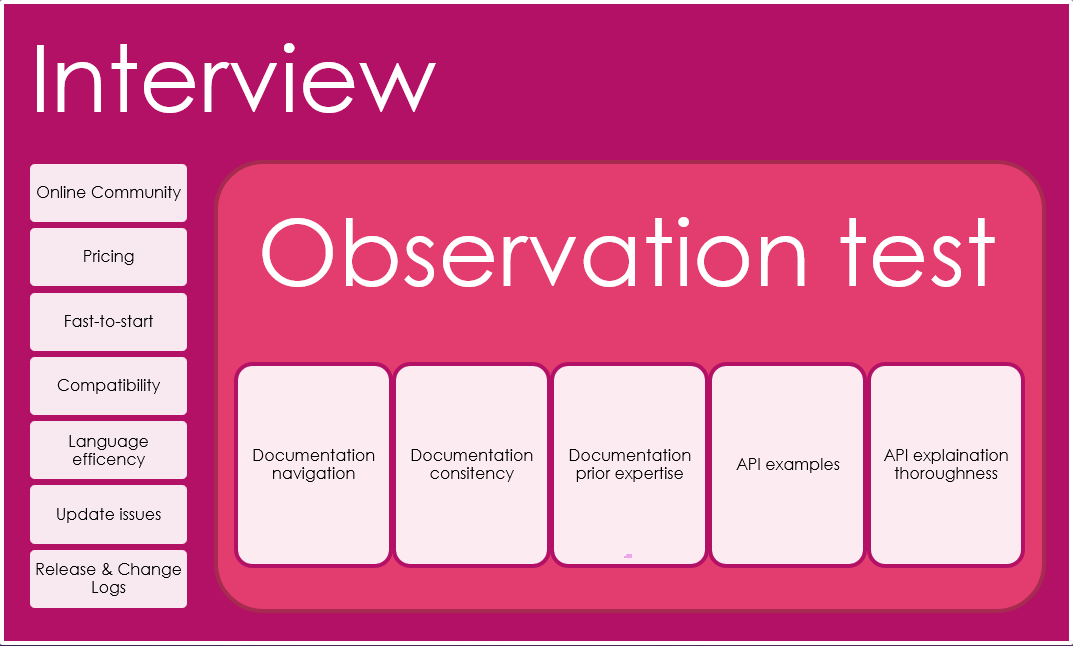
\includegraphics[width=\linewidth]{obsVSinterview.png}
\caption{What was easy to explore with interviews, compared with observation studies}
\label{fig:obsVSinter}
\end{figure}
\subsubsection{Interview Decisions}
There are several things we had to decide when were going to do interviews. This included what type of interview style we wanted to use, what structure the interview should have, what subjects should be explored and what questions should be asked.
\paragraph{Interview Style}
There are many different ways of conducting interviews. \cite{denscombe} groups it into
three different approaches: one-on-one interviews, group interviews and focus groups.
These methods all have pros and cons, described by Denscombe.
\\ \\
One-on-one interviews are easy to arrange, since
only two people's (Interviewer and interviewee) schedules have to coincide.
Compared to group interviews and focus groups, it's also easy to control the interview,
dive deeper into questions when needed and it's easy to link the results
to the specific person.
\\ \\
Group interviews have advantages as well. It helps to find what a consensus around
a topic is, where people's opinions can be challenged right away by other group members.
There are also risks of group interviews, where 'quieter' people may be silenced by
members of the group who are more dominant. Group interviews are also less suited
for topics where answers that are more 'accepted' than others.
\\ \\
Finally, focus groups have the same issues as group interviews does. It also
requires a more skilled moderator, since focus groups is more of an ongoing
discussion of experts within a field, that can easily get out of hand if the
moderator does not know how to steer the group.  Transcribing focus groups are also
more challenging since it is natural that people talk over each other. Linking opinions
to certain people may also be harder when everyone's statements are blurred together.
\\ \\
For this research project we chose to go ahead with one-on-one interviews.
The disadvantages of them are small, and one the most challenging things
about the interviews is finding time to arrange them. It was not feasible
to try to find enough people for a group interview where everyone's schedules
could coincide.
\paragraph{Interview Structure}
Dencsombe describes three different types of interviews: structured, semi-structured and
unstructured interviews. Structured interviews are much like questionnaires, where
the interviewer holds a tight grip on the interview and does not expect free form answers.
Structured interviews looks to standardize the results for easy comparison.
This interview structure is more for 'checking' rather than 'discovery' and is
therefor more of a quantitative data collection rather than qualitative.
\\ \\
Semi-constructed interviews has, just like constructed interviews, a clear set
list of questions. However, in a semi-structured interview, the interviewee
is not presented with yes or no questions, or questions with alternatives.
The questions are instead open-ended. As described by \cite{denscombe}, the interviewee
is expected to develop their own ideas and speak widely about the given issue or question.
Here, the emphasis is more on 'discovery' than checking.
\\ \\
Unstructured interviews is the third alternative and is the loosest of the three styles.
With this structure, the interviewer wants to get the interviewees general thoughts
on a subject or issue and tries to be as unobtrusive as possible. As described by \cite{denscombe},
the interviewer presents a specific issue or subject and hopes to get a ball rolling.
Semi-constructed and unstructured exist on a continuum. The more open-ended the questions
are, the more you move from semi-structured to to unstructured.
\\ \\
For this research project we are using the style of semi-constructed.
We are trying to discover things rather than check, which removes the option
of a structured interview. We however have a very clear set of questions
we want answers on.

\subsubsection{Interview Subjects}
There are many things that be explored for these interviews. Due to limited
time, we had to narrow it down to a few subjects. The three subjects
we chose are related to release notes, APIs and online community.
\\ \\
Release notes is noted as a very important aspect by literature, but
the survey results show that this is one of the least considered aspects.
Our theory is that this is because people don't look
at release notes until they are needed, and don't usually consider this
when choosing platforms. However, a more surprising part is that it does \textit{not}
affect them negatively DX-wise either if the release notes are poorly written.
To get a deeper understanding on why this is, we chose this as a subject
for the interviews.
\\ \\
The API documentation and examples are pointed as very important by the
surveys. In the survey we used the vague term of 'Good' and 'Bad', and
the survey takers applied their own definition of these two terms. We
are interested of how we can define 'Good' and 'Bad'. One of the most important
aspects according the survey is also to have working code quickly. Upon exploring
possible aspects to explore, we found ourself asking if working code quickly
is jus ta consequence of good API documentation and examples. Maybe it's not
its own aspect at all? So this question also got merged into this question subject.
\\ \\
The last subject we chose to explore is online communities. An anomaly found
between the first and second survey is that online community was very important
to people in the first survey, but only somewhat important in the second one.
We want to understand the shift in this ranking.

\subsubsection{Interview material}
We concluded that it would be good to have reference points during the interview,
that there should be some material that the interviewee could use when talking.
We discussed using some API documentation and release notes from existing software platforms,
more precisely Qlik Core. However, Qlik Core is a very advanced platform which takes a long time
to grasp. Since the interviewees have limited time to put aside for the interviews, it seemed
like making them read and understand documentation of a whole new software platform was too much to ask.
Instead we created some API documentation and release notes for a made up software platform
called 'MyBakery'. Everyone already have a good mental picture of how a bakery works,
so even if you give them limited amount of documentation they still have a mental picture
of what this software platform does. To make the request of making them read documentation less boring,
we tried to make a gamification of the task. The interviewees were given the material, and
three questions they needed to answer. This forced them to read and understand the material, rather
than just read through it. The material can be seen in appendix X.

\subsubsection{Interview Questions}

Ultimately, we want to answer "Why are the aspects needed or not needed
to give a good DX and what happens if they (don’t) exist or are poorly/well implemented?"
The questions for the interviews were constructed to be able to answer this question.
Since the interview is semi-constructed, all questions will not necessarily be asked.
Depending on how the interviewee answer, some questions may already have been answered,
some questions may be uninteresting to dive into, etc.
\paragraph{A - APIs}
For the API documentation, API examples and to have working code quickly, we
already knew that is important. It wasn't very surprising that it was.
For this, we were rather trying to understand how we define 'Good' API related things.

\begin{enumerate}[label={A\Alph*}]
\item \textbf{General}
\begin{enumerate}[label={AA\arabic*}]
\item How important would you say API documentation and examples are?
\end{enumerate}
\item \textbf{Api Documentation}
\begin{enumerate}[label=AB\arabic*]
\item When you look at API documentation, what are you usually looking for?
\begin{itemize}[label={-}]
\item What should the documentation look like?
\item Is there anything in the material you always look for, or something that is missing?
\item When you come across an API documentation, are there any red flags you look for?
\end{itemize}
\item	How does the API documentation quality affect you in your work?
\begin{itemize}[label={-}]
\item Do you abandon a software platform if the documentation is poor?
\end{itemize}
\end{enumerate}
\item \textbf{Api Examples}
\begin{enumerate}[label={AC\arabic*}]
\item	What is your goal when looking at API examples?
\begin{itemize}[label={-}]
\item For copy-pasting?
\item To understand underlying structure?
\item To simply see how it's used?
\end{itemize}
\item   What should API examples look like?
\begin{itemize}[label={-}]
\item Short examples or long examples?
\item Should it be runnable or concise?
\item Within a big context or concise?
\end{itemize}
\item	How does the API examples quality affect you in your work?
\begin{itemize}[label={-}]
\item Do you abandon a software if the examples are poor?
\end{itemize}
\end{enumerate}

\item\textbf{Working Code Quickly}
\begin{enumerate}[label={AD\arabic*}]
\item Is it important for you to have working code quickly?
\begin{itemize}[label={-}]
\item Why is it/is it not?
\end{itemize}
\item When can you accept to not have working code quickly?
\item Can you have working code quickly if the API examples and documentation is bad?
\end{enumerate}
\end{enumerate}

\paragraph{B - Release Notes}
For release notes, we know through the survey that they are \textit{not} considered.
The questions have been divided into three groups: 'When are [release notes] needed",
"What should [release notes] look like?". We also asked a final question to see if the interviewee had any ideas about anomalies in the surveys.

\begin{enumerate}[label=B\Alph*]
\item \textbf{BA - When are they used?}
\begin{enumerate}[label=BA\arabic*]
\item How often do you look at release notes?
\item In what circumstances do you look at release notes?
\begin{itemize}[label={-}]
\item Do you look at release notes before deciding to use a platform?
\end{itemize}
\item What do you look for when looking at release notes?
\end{enumerate}
\item \textbf{What should they look like?}

\begin{enumerate}[label=BB\arabic*]
\item Would you say it is important that software platforms have release notes?
\begin{itemize}[label={-}]
\item Do you find that information in some other way?
\end{itemize}
\item How detailed should they be? / What should they look like?
\begin{itemize}[label={-}]
\item How important is it for you that the release notes are thoroughly written?
\end{itemize}
\item Is it worth a company's time to make thorough release notes?
\item How do poor release notes affect you?
\end{enumerate}
\item \textbf{Survey Anomaly}
\begin{enumerate}[label=BC\arabic*]
\item Release notes is ranked as the least, or amongst the least important aspect for all groups. Why do you think that is?
\end{enumerate}
\end{enumerate}


\paragraph{C - Online Communities}
For online community, we are trying to understand why it was ranked
so differently in the two surveys. We also try to understand why, in general,
an online community matters.

\begin{enumerate}[label=C\Alph*]
\item \textbf{General}
\begin{enumerate}[label={CA\arabic*}]
\item	When talking about software platforms, what is an online community to you?
\item	If the documentation was flawless, would you not need an online community?
\end{enumerate}
\item \textbf{When are they used?}
\begin{enumerate}[label={CB\arabic*}]
\item	How often would you say you take help from online communities?
\item   Do you check out the online community before choosing a platform?
\end{enumerate}
\item \textbf{What should it look like?}

\begin{enumerate}[label=CC\arabic*]
\item	What do you want from an online community / what should it look like?
\begin{itemize}[label={-}]
\item How important are online communities?
\item What do communities that you like have in common?
\item Is it important that a community feels alive?
\item Is it important the community feels helpful?
\item Is it important that the tone used in the community is positive?
\item Is it important that the company behind the software are part of the community?
\end{itemize}
\item	If we compare software platforms to something smaller, such as a library. Would you say it is more important or less important to have a software community around it?
\begin{itemize}[label={-}]
\item Why is it more/less important?
\end{itemize}
\end{enumerate}
\item \textbf{Survey Anomaly}
\begin{enumerate}[label={CD\arabic*}]
\item In the first survey, having an online community was ranked as the second most important aspect. In the second one, it’s ranked in the middle. Why do you think that is?
\end{enumerate}
\end{enumerate}

\subsection{Evaluating Qlik Core}

More text here...

\section{Results and Discussion}

\subsection{Initial Survey}
Although the first survey only was a pilot version, it can be interesting to evaluate the results of it. There were also things asked in the first survey, that wasn't in the main one. We got 38 responses in total.
Initially we intended to look at the outcome from four different perspectives, and compare them to the overall group. The four perspectives were:
\begin{itemize}[label={}]
\item People with more than 5 years experience in the industry
\item People who are developers within the industry
\item People who are architects within the industry
\item People in companies with more than 200 employees
\end{itemize}
The last perspective with the larger companies was
scrapped since the majority of all answers were from Qlik, and the group
was therefor a too big majority of the whole group.

The survey found that the majority of people do not know what DX is. In table \ref{tab:knowdx} we can see how many people felt they could define DX. As we can see, it's quite an unknown term. Almost half had not heard of it, and only 7.9\% felt they fully knew what it was.

\begin{table}[H]
\centering
\begin{tabularx}{\columnwidth}{X|l}
\multicolumn{2}{c}{\textbf{Have you heard of the term 'Developer Experience'?}} \\ \hline \hline
\textbf{Answer} & \textbf{Percent} \\ \hline
Yes, and I could comfortably give a definition of it & 7.9\%  \\ \hline
Yes, and I think I could give a definition of it & 	21.1\%  \\ \hline
Yes, but I could not give a definition of it &	18.4\%  \\ \hline
No &	47.4\%  \\ \hline
I don't know & 5.3\% \\ \hline
\end{tabularx}
\caption{Percent of people who knew what Developer Experience was.}
\label{tab:knowdx}
\end{table}

\subsubsection{Consideration Factors}
The scores from consideration question in the first survey in figure \ref{fig:scopresByPoints}. The table is divided into the different perspectives. "Everyone" is simply the average result, "Experienced" is people with more than 5 years of experience in the industry, "Developers" are those who had the job title of developer or software engineer, and "Architects" are those who were some for of software architect.
As we can see, all but 3 factors scored equal to or above 0.50 points, meaning that they
were factors that were more often than not considered.
\begin{figure}[H]
\centering
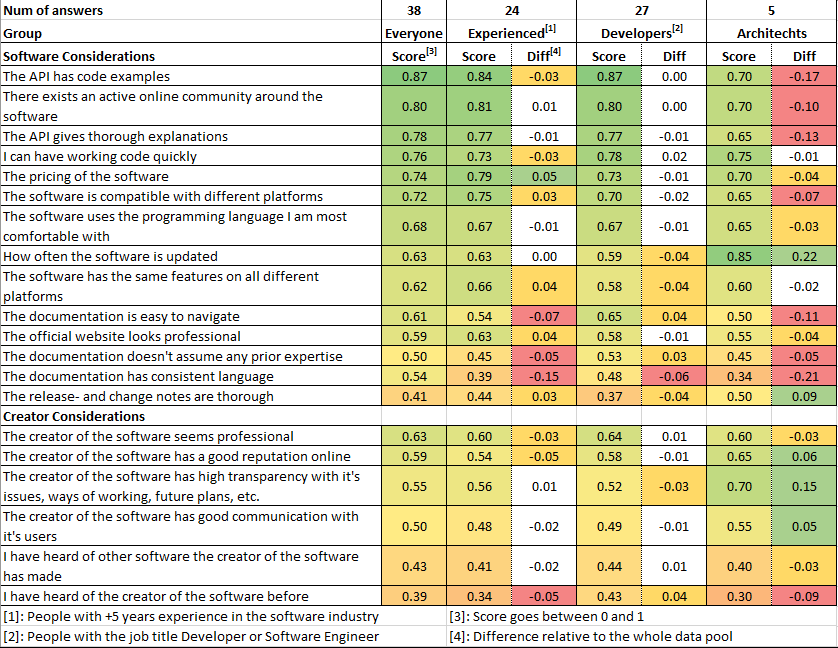
\includegraphics[width=\linewidth]{ScoresByPoints.png}
\caption{Scores from consideration aspects in survey 1, divided into different perspectives.}
\label{fig:scopresByPoints}
\end{figure}
If we start by looking at the software consideration aspects, we can see that the most important
factor was 'The API has code examples', followed by the importance of an
active community around the software, and thirdly that the API
explanations were thorough. The least two important factors were 'The
documentation has consistent language' and 'The release- and change
notes are thorough'.
This is an interesting find, since literature highlights these to factors as being very important. Many companies also spend a lot of resources to keep documentation up-to-date and release notes thorough. Here we see that most people, more often than not, do \textit{not} consider this factor. A potential explanation to this could be that the question is phrased so that it puts the emphasis on \textit{try} a new software, whereas these two factors may be only relevant in long term use of a software. As we'll see in the main survey however, where the question was phrased as \textit{use a software platform}, release notes were once again listed as one of the least important aspects.
\\ \\
For the more experienced users, the result differ some when compared to the 'Everyone' group. They take less consideration to factors surrounding APIs, documentation and time to get started, and care more about pricing,
cross-platform compatibility and the thoroughness of release notes.
\\ \\
With the group consisting of mainly developers, we see almost the
inversion of some trends in the more-experience-group. The developer
group cares about documentation and time-to-get-started, and do not care
about release notes and cross-platform compatibility.
\\ \\
If we look at the part about the creator behind the software, we can deduct a few things.
Overall, the creator behind the software seem to be not completely non-important,
but also not very important, with all factors scoring close to 0.50. The most
commonly considered factor was that the creator seemed professional, but
that only ranked 0.63 on average. The least considered factor was 'I have heard of
the creator of the software before', which ranked only 0.39.
\\ \\
With the more experienced users, they considered the factors even more
rarely than the 'Everyone' group, apart from transparency, which increased
slightly. Still, the scores are close to 0.50, and the creator once again
seem to be only a somewhat important factor.
\\ \\
With the group consisting of only developers, it's much the same as
before, with the one exception that 'I have heard of the creator of the
software before' had an increase by 10\%. It is however still the least
considered factor.
\subsubsection{Deal Breakers}
The first survey also had a section of what they considered to be a deal breaker for trying out a new software.
In table \ref{tab:dealbreaker} we can see the result of this.

\begin{table}[H]
\centering
\begin{tabularx}{\columnwidth}{r X}
& \textbf{Aspect}	\\ \hline
70\%	&	I have to pay to be able to fully evaluate the software	\\
65\%	&	It takes a long time to get initially started	\\
65\%	&	The API is poorly explained	\\
62\%	&	The API has poor or no code examples	\\
59\%	&	The online community around the software is dead or has little activity	\\
27\%	&	The creators behind the software feel like they cater to businesses, not developers	\\
27\%	&	The online community around the software is unappealing	\\
16\%	&	The website for the documentation is hard to navigate	\\
11\%	&	The documentation uses inconsistent language	\\
11\%	&	The software is not open source	\\
8\%	&	The creators behind the software are not transparent	\\
8\%	&	The documentation assumes prior experience with the software	\\
3\%	&	The release notes are poorly written	\\ \hline
\end{tabularx}
\caption{Percentage of people who found aspects to be a deal breaker}
\label{tab:dealbreaker}
\end{table}

As we can see much of the things that people consider when choosing a software is also a deal breaker if it's poorly implemented. A very clear result from this part is that most people are \textit{not} willing to pay for a software before they can try it out.

\subsubsection{Ways of Finding New Software}
In the test survey there was also a part about how people find new software. The answers can be seen in table \ref{tab:discover}. As we can see, the most common way of finding new software is either through people you know, or online discussions. Since people spend the majority of their working time online and with coworkers, this is quite a natural result. Conferences and online courses are not part of people's daily lives in the same way, and naturally it's not a common source of new discovering new software.

\begin{table}[H]
\centering
\begin{tabularx}{\columnwidth}{X|l}
\multicolumn{2}{c}{\textbf{How do you usually discover new tools and frameworks?}} \\ \hline \hline
\textbf{Answer} & \textbf{Percent} \\ \hline
Friends or coworkers telling me about it	&	86.8\% \\
Online communities and forums	&	86.8\% \\
Reading blog posts or articles	&	55.3\% \\
Searching for related key words online	&	50.0\% \\
Social media	&	34.2\% \\
Conferences	&	26.3\% \\
Online Courses	&	13.2\% \\ \hline
\end{tabularx}
\caption{The most common ways of finding new software}
\label{tab:discover}
\end{table}

\subsection{Survey 2 Results}
There are many ways you can view the results. We've tried to look at it from many different angles, and compare it with different groups. \\
In total, the main survey yielded 39 responses. The results were loaded into Qlik Sense
where we could find different groups and patterns. We looked at the
results from three angels: The overall average result, result depending
on your job title and result depending on how much experience you have
in the industry.
\\ \\
The job titles were divided into four groups: Architects, Developer and
Engineers, Managers and Other. The quantity and percentage of total can
be seen in the table \ref{tabl:jobs}.

\begin{table}[H]
\centering
\begin{tabularx}{\columnwidth}{r l l}
\textbf{Grouped Job Titles} &    \textbf{\# of answers} &     \textbf{\% of total} \\\hline
Architects              & 10           & 25.6\%  \\ \hline
Developer and Engineers & 21           & 53.8\%  \\\hline
Managers                & 4            & 10.3\%  \\\hline
Other                   & 4            & 10.3\%  \\\hline
\end{tabularx}
\caption{Main survey responses grouped by job titles}
\label{tabl:jobs}
\end{table}

In table \ref{tab:allPoints} we can see all the aspects, what points each job title gave it and
their ranking.

\begin{table}[H]
\centering
\begin{tabular}{c|r:l|r:l|r:l|r:l|r:l}
\multicolumn{11}{c}{\textbf{Aspects with their ID}} \\  \hline
1   & \multicolumn{10}{l}{How often the software is updated}                                        \\
2   & \multicolumn{10}{l}{I can have working code quickly}                                           \\
3   & \multicolumn{10}{l}{The API documentation gives thorough explanations on how it works}        \\
4   & \multicolumn{10}{l}{The API has code examples}                                                \\
5   & \multicolumn{10}{l}{The documentation doesn't assume any prior expertise}                      \\
6   & \multicolumn{10}{l}{The documentation has consistent language}                                 \\
7   & \multicolumn{10}{l}{The documentation is easy to navigate}                                       \\
8   & \multicolumn{10}{l}{The official website looks professional}\\
9   & \multicolumn{10}{l}{The pricing of the software}\\
10  & \multicolumn{10}{l}{The release- and change notes are thorough}\\
11  & \multicolumn{10}{l}{The software has the same features on all different platforms}\\
12  & \multicolumn{10}{l}{The software is compatible with different platforms}\\
13  & \multicolumn{10}{l}{The software is offered in more than one programming language}\\
14  & \multicolumn{10}{l}{The software is open source}\\
15  & \multicolumn{10}{l}{The software uses the programming language I am most comfortable with} \\
16  & \multicolumn{10}{l}{There exists an active online community around the software}\\ \hline
\multicolumn{11}{c}{} \\
\multicolumn{11}{c}{\textbf{Scores and rankings}} \\  \hline
\rotatebox{90}{Aspect ID}                                & \rotatebox{90}{Everyone Rank } & \rotatebox{90}{Avg Everyone } & \rotatebox{90}{Architects Rank } &\rotatebox{90}{Architects Score } & \rotatebox{90}{D\&E* Rank } & \rotatebox{90}{D\&E* Score } &  \rotatebox{90}{Managers Rank } & \rotatebox{90}{Managers Score } & \rotatebox{90}{Other Rank } & \rotatebox{90}{Other Score }\\ \hline
4                                             &             1 & 0.90         &         1 &   0.92       &            1 & 0.91       &        1 & 0.79     &        1-2 & 0.94  \\ \hline
3     &             2 & 0.82         &         3 &   0.82       &            2 & 0.87       &        3 & 0.73     &          4 & 0.74  \\ \hline
2                                       &             3 & 0.80         &         2 &   0.85       &            4 & 0.80       &      4-5 & 0.71     &        1-2 & 0.94  \\ \hline
9                                           &             4 & 0.80         &         5 &   0.76       &            3 & 0.84       &        2 & 0.75     &          3 & 0.85  \\ \hline
15 &             5 & 0.68         &         6 &   0.69       &            5 & 0.73       &      6-7 & 0.63     &          5 & 0.69  \\ \hline
14                                           &             6 & 0.68         &         4 &   0.77       &            6 & 0.69       &        8 & 0.60     &          8 & 0.58  \\ \hline
16           &             7 & 0.65         &         8 &   0.63       &            7 & 0.67       &     9-11 & 0.54     &          6 & 0.65  \\ \hline
7                                 &             8 & 0.60         &         7 &   0.66       &            8 & 0.61       &       12 & 0.52     &         10 & 0.52  \\ \hline
8                               &             9 & 0.60         &         9 &   0.63       &           10 & 0.56       &      4-5 & 0.71     &         12 & 0.44  \\ \hline
12                   &            10 & 0.58         &        10 &   0.58       &           11 & 0.52       &     9-11 & 0.54     &          7 & 0.59  \\ \hline
1                                    &            11 & 0.58         &        11 &   0.52       &            9 & 0.57       &      6-7 & 0.63     &         11 & 0.51  \\ \hline
5                  &            12 & 0.47         &        13 &   0.47       &           13 & 0.44       &     9-11 & 0.54     &          9 & 0.52  \\ \hline
11         &            13 & 0.46         &        14 &   0.41       &           12 & 0.45       &    13-15 & 0.44     &         13 & 0.42  \\ \hline
6                             &            14 & 0.41         &        12 &   0.49       &           14 & 0.34       &       16 & 0.42     &         14 & 0.39  \\ \hline
13         &            15 & 0.36         &        15 &   0.37       &           15 & 0.31       &    13-15 & 0.44     &         16 & 0.23  \\ \hline
10                            &            16 & 0.33         &        16 &   0.26       &           16 & 0.29       &    13-15 & 0.44     &         15 & 0.35  \\ \hline \hline
\multicolumn{11}{l}{*D\&E: Developers and Engineers}
\end{tabular}
\caption{List of aspects with their ID, and points and rankings of aspects, grouped by job title}
\label{tab:allPoints}
\end{table}


\subsubsection{Overall Result}
Overall, there were quite a lot of interesting findings when analyzing the results from the main survey.
In general, people are more likely to consider things when they are choosing for
a group rather than for themselves. For the three categories, Single is the
closest to the average result, with Group and Hobby existing as
opposites on either side of Single. In all but one case, if it's often
considered when choosing for a group, it's \textit{not} often considered when choosing
for a hobby project, and vice versa.
\\ \\
For the part of the survey regarding DX and people's feelings around software platforms, it can be said that there is a direct correlation between if an aspect in it's good form has a positive impact, that same aspect in it's
bad form will have about the same level of negative impact.
However, in all but once case, the positive effect is greater than the negative
effect, if only slightly. In general it is closely related to how often
something is considered. That is to say, if something will cause someone to have a non-neutral feeling regarding an aspect, they will also consider it when choosing a platform. Ergo, there is no uncoupling between what causes them to have a good DX, and what they consider when choosing a platform. There are some
outliers to this, but that is the general case.
\\ \\
The top three most considered aspects for each context can be seen in
the table \ref{tabl:top3}.

\begin{table}[H]
\centering
\begin{tabular}{r l}
\hline\hline
\multicolumn{2}{c}{\textbf{Average}} \\ \hline
1 &The API has code examples \\
2 & The API documentation gives thorough explanations on how it works \\
3 &I can have working code quickly \\
\hline\hline
\multicolumn{2}{c}{\textbf{Group}} \\ \hline
1 & The API has code examples                                        \\
2 & The API documentation gives thorough explanations on how it works \\
3 & The software is compatible with different platforms              \\
\hline\hline
\multicolumn{2}{c}{\textbf{Single}} \\ \hline
1 &  The API has code examples                                         \\
2 &  The API documentation gives thorough explanations on how it works  \\
3 &  I can have working code quickly                                   \\
\hline\hline
\multicolumn{2}{c}{\textbf{Hobby}} \\ \hline
1 & The pricing of the software    \\
2 & The API has code examples       \\
3 & I can have working code quickly\\ \hline
\end{tabular}
\caption{Top 3 considered aspects by each context}
\label{tabl:top3}
\end{table}
The overall result concluded that \textit{the} most considered aspect overall
is 'The API has code examples'. For hobby, it's the second most
important aspect, losing the first place by only 0.03 points.
Further, good code
examples had the biggest positive impact on developer experience, and
bad code examples had the biggest negative impact on DX. The negative
impact if the examples are bad are not as extreme as the positive impact
is if they are good however. In conclusion, API examples are a key
factor for software platforms' quality.
\\ \\
The thoroughness of the documentation is also one of the most important
aspects, coming in as the second most important aspect for all
categories except for Hobby. The positive DX-impact is as big as the
negative one, and it's also reflected in that it's consideration points
are as high as the DX-impact points.
\\ \\
Having working code quickly is also in the top three for all but the
group category, where it's in fourth place. The positive DX-impact if
you can have working code quickly is slightly higher than the negative
DX-impact if it takes a long time before you have working code. The
positive impact is also stronger than if you compare it to how often
it's considered.
\\ \\
Having the software be compatible with different platforms is a big
divider. It's the third most important aspect for Group, but one the
least important aspects for Hobby, and somewhere in the middle for
Single. The positive impact is lower than how often it's considered, and
the negative DX-impact is even less. If you exclude the Group-category,
it places itself on average as the 11\textsuperscript{th} most important
aspect, out of 16.
\\ \\
The pricing of the software is important to everyone, placing itself on
average as the 4\textsuperscript{th} most important aspect overall, but it is \textit{the}
most important aspect for Hobby. For group and single, it's both the
5\textsuperscript{th}  and 4\textsuperscript{th}  most important aspect respectively.

In figure \ref{fig:dxandcosnid} you can see how the consideration points compares to how much of a positive and negative DX impact it has. In table \ref{tab:dx} you can see the exact numbers for the DX impacts, and the average scores. As we can see, the difference in positive- and negative DX impact is quite small.\\ \\

There are several angles you can view the results at. Here we discuss a few.
\begin{table}[H]
\centering
\begin{tabularx}{\columnwidth}{l|X r r r r}
\textbf{\rotatebox{90}{Aspect ID}} & \textbf{Aspect Category}	&	\textbf{\rotatebox{90}{Average Score}}	&	\textbf{\rotatebox{90}{Negative DX}}	&	\textbf{\rotatebox{90}{Positive DX}}	&	\textbf{\rotatebox{90}{DX Diff}}	\\ \hline
4   & Api Code Examples	&	0.89	&	0.85	&	0.89	&	\pm 0.04	\\ \hline
3  & Working Code Quickly	&	0.85	&	0.83	&	0.82	&	\pm 0.01	\\ \hline
2  & Documentation Thoroughness	&	0.83	&	0.80	&	0.81	&	\pm 0.01	\\ \hline
9  & Pricing	&	0.76	&	0.74	&	0.81	&	\pm 0.07	\\ \hline
15  & Documentation Navigation	&	0.72	&	0.64	&	0.70	&	\pm 0.06	\\ \hline
14 & Updates	&	0.72	&	0.63	&	0.69	&	\pm 0.04	\\ \hline
16  & Online Community	&	0.71	&	0.62	&	0.65	&	\pm 0.03	\\ \hline
7  & Favourite Programming Language	&	0.67	&	0.62	&	0.60	&	\pm 0.02	\\ \hline
8  & Being Open Source	&	0.66	&	0.59	&	0.59	&	0.00	\\ \hline
12 & Official Website Look	&	0.63	&	0.56	&	0.56	&	0.00	\\ \hline
1  & Documentation Language Consistency	&	0.63	&	0.53	&	0.55	&	\pm 0.02	\\ \hline
5  & Features On All Platforms	&	0.63	&	0.53	&	0.48	&	\pm 0.05	\\ \hline
11 & Documentation Prior Expertise	&	0.57	&	0.47	&	0.43	&	\pm 0.03	\\ \hline
6   & Platform Compatibility	&	0.47	&	0.42	&	0.41	&	\pm 0.01	\\ \hline
13 & Release Notes	&	0.44	&	0.40	&	0.34	&	\pm 0.06	\\ \hline
10 & Number of Programming Languages	&	0.39	&	0.34	&	0.32	&	\pm 0.02	\\ \hline
\end{tabularx}
\caption{The average scoring, its positive DX impact and its negative DX impact and their difference, by each aspect category}
\label{tab:dx}
\end{table}


\begin{figure}[H]
\centering
\begin{tabular}{r l}
\hline
1    & How often the software is updated    \\
2    & I can have working code quickly  \\
3    & The API documentation gives thorough explanations on how it works    \\
4    & The API has code examples    \\
5    & The documentation doesn't assume any prior expertise \\
6    & The documentation has consistent language    \\
7    & The documentation is easy to navigate    \\
8    & The official website looks professional  \\
9    & The pricing of the software  \\
10    &  The release- and change notes are thorough \\
11   &  The software has the same features on all different platforms   \\
12    &  The software is compatible with different platforms    \\
13  &  The software is offered in more than one programming language    \\
14    &  The software is open source    \\
15    &  The software uses the programming language I am most comfortable with  \\
16    &  There exists an active online community around the software    \\ \hline
\end{tabular}
\hspace*{-0.25\textwidth}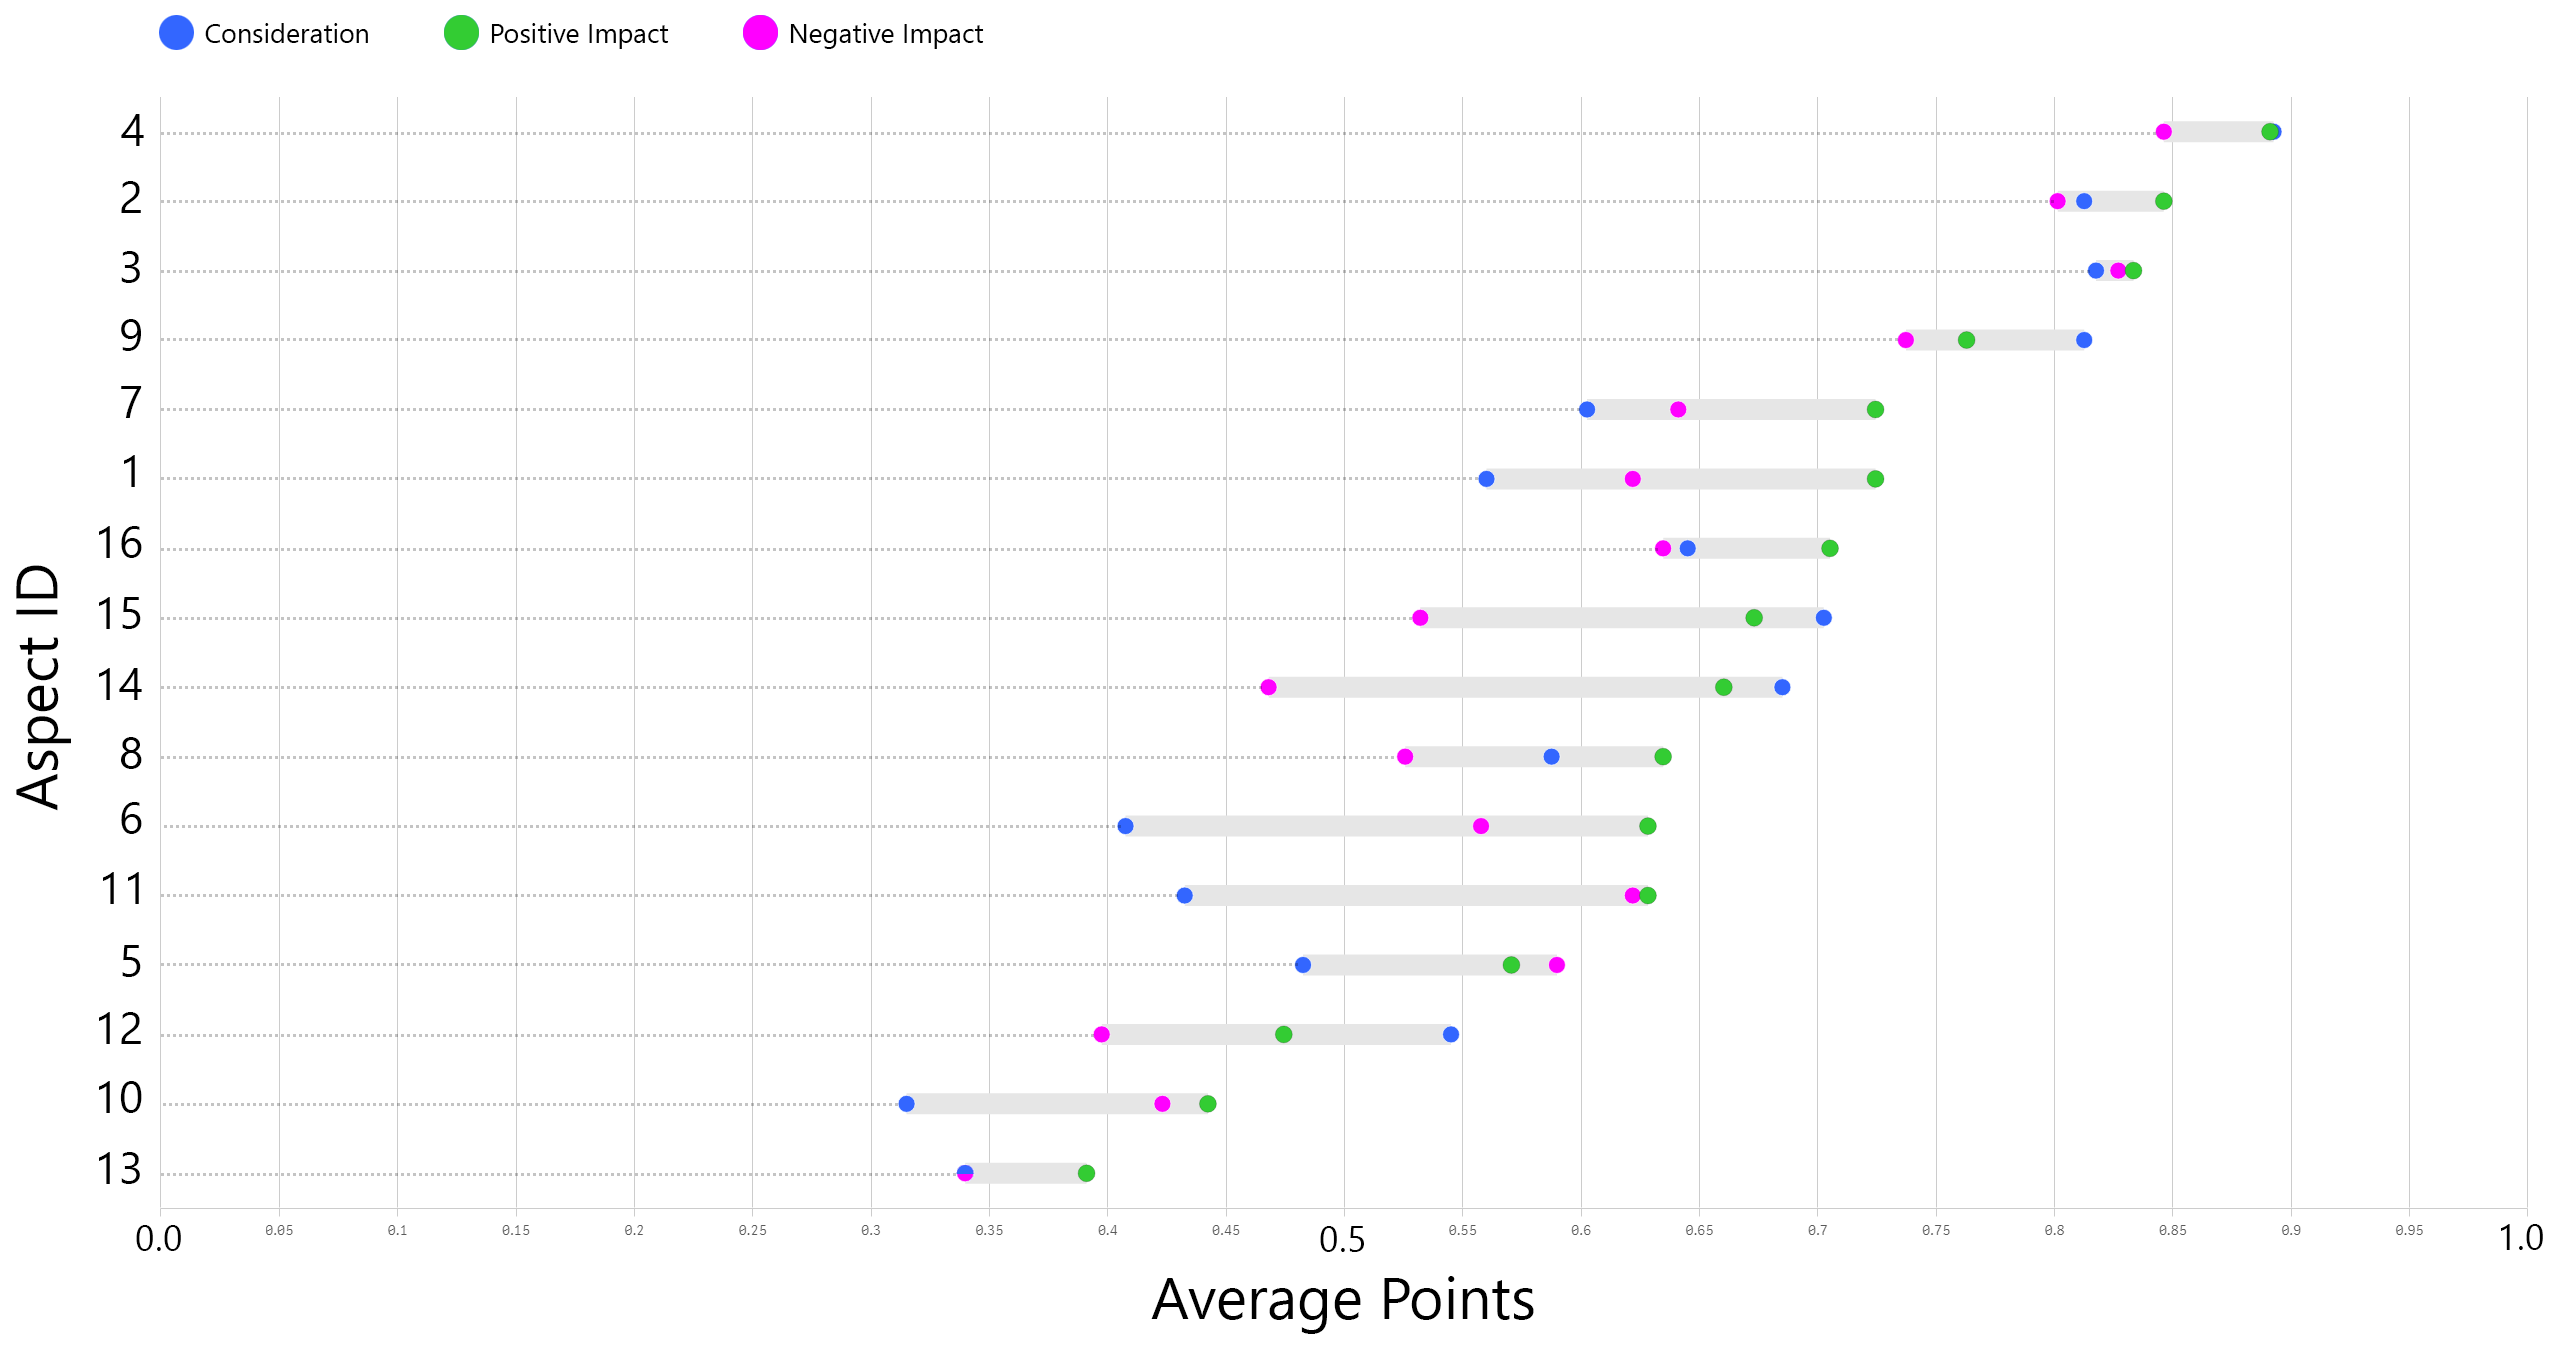
\includegraphics[width=1.5\textwidth]{dxandconsid.png}
\caption{The scoring of the consideration points, with how much of a positive- and negeative DX impact it has.}
\label{fig:dxandcosnid}
\end{figure}

\subsubsection{Developer and Engineers}
Developer and Engineers are the majority of people who are going to use a software platform, since they make out the majority of a development team. In the survey, they also made out the majority of the respondents. In table \ref{tab:devs} we can see how they ranked the considerations. According to this, they are people who want thorough documentation and API examples. They want to have working code quickly, and they care about the pricing of the software. They also more often than not care if a project is open-source, and also want to use the programming language they are most comfortable with. Even though they want thorough documentation, less often than not they don't care if the documentation uses inconsistent language or assumes prior expertise. They do not care if release notes are thorough. Developers and engineers have an average score of 0.60, with the difference between the most considered thing, and the least considered thing, being 0.62.

\begin{table}[H]
\centering
\begin{tabularx}{\columnwidth}{ l X r}

{\textbf{R}*} &   \textbf{Aspect}   & {\textbf{S}**} \\ \hline
1 &      The API has code examples                                             &  0.91             \\ \hline
2 &      The API documentation gives thorough explanations on how it works     &  0.87             \\ \hline
3 &      The pricing of the software                                           &  0.84             \\ \hline
4 &      I can have working code quickly                                       &  0.80             \\ \hline
5 &      The software uses the programming language I am most comfortable with &  0.73             \\ \hline
6 &      The software is open source                                           &  0.69             \\ \hline
7 &      There exists an active online community around the software           &  0.67             \\ \hline
8 &      The documentation is easy to navigate                                 &  0.61             \\ \hline
9 &      How often the software is updated                                     &  0.57             \\ \hline
10 &      The official website looks professional                               &  0.56             \\ \hline
11 &      The software is compatible with different platforms                   &  0.52             \\ \hline
12 &      The software has the same features on all different platforms         &  0.45             \\ \hline
13 &      The documentation doesn't assume any prior expertise                  &  0.44             \\ \hline
14 &      The documentation has consistent language                             &  0.34             \\ \hline
15 &      The software is offered in more than one programming language         &  0.31             \\ \hline
16 &      The release- and change notes are thorough                            &  0.29             \\ \hline \hline
\multicolumn{3}{l}{*R: Rank, **S: Score}
\end{tabularx}
\caption{The ranking and scores of developers and engineers}
\label{tab:devs}
\end{table}

\subsubsection{Architects}
Architects are a key part of a development team. They are responsible for how the software will be structured and therefor also often have a say in, if the software will be using a software platform, what platform will be used. In table \ref{tab:arch} we can see how the architects ranked the aspects. According to this result, architects are (just like developers) people who want code examples and thorough documentation. They find it important that software platforms are open-source, and want to have working code quickly. They also, just like developers, do not care if the release notes are thorough. The average score for architects is 0.61, with the a difference between the most considered thing, and the least considered thing, of 0.66.

\begin{table}[H]
\centering
\begin{tabularx}{\columnwidth}{l X r}

\textbf{R}* &  \textbf{Aspect}        & \textbf{S}** \\ \hline
1 &    The API has code examples                                             &         0.92             \\ \hline
2 &    I can have working code quickly                                       &         0.85             \\ \hline
3 &    The API documentation gives thorough explanations on how it works     &         0.82             \\ \hline
4 &    The software is open source                                           &         0.77             \\ \hline
5 &    The pricing of the software                                           &         0.76             \\ \hline
6 &    The software uses the programming language I am most comfortable with &         0.69             \\ \hline
7 &    The documentation is easy to navigate                                 &         0.66             \\ \hline
8 &    There exists an active online community around the software           &         0.63             \\ \hline
9 &    The official website looks professional                               &         0.63             \\ \hline
10 &    The software is compatible with different platforms                   &         0.58             \\ \hline
11 &    How often the software is updated                                     &         0.52             \\ \hline
12 &    The documentation has consistent language                             &         0.49             \\ \hline
13 &    The documentation doesn't assume any prior expertise                  &         0.47             \\ \hline
14 &    The software has the same features on all different platforms         &         0.41             \\ \hline
15 &    The software is offered in more than one programming language         &         0.37             \\ \hline
16 &    The release- and change notes are thorough                            &         0.26             \\ \hline \hline
\multicolumn{3}{l}{*R: Rank, **S: Score}
\end{tabularx}
\caption{The ranking and scores of architects}
\label{tab:arch}
\end{table}

\subsubsection{Managers}
Managers have responsibilities that differ quite much from developers, engineers and architects. They often have to think of legal aspects and are in contact with other departments, such as sales. They will often also not have the same level of competence when it comes to software development as architects, developers and engineers have. They are also not the key demographic for this research, since we are talking about \textit{developer} experience. They are however a key part for the selection of software platforms, since they will have the most authority and also are the person in control (or is the contact to the person in control) of the money. In table \ref{tab:managers} we can see how the managers ranked the aspects. There we can see that even managers care about API examples and that they can have working code quickly. The pricing of the software is, maybe not surprisingly, quite important to them. Managers have an average score of 0.59, with the biggest difference between the most considered thing, and the least considered thing, being just 0.37.

\begin{table}[H]
\centering
\begin{tabularx}{\columnwidth}{l X r}

\textbf{R}* &  \textbf{Aspect}        & \textbf{S}** \\ \hline
1 &   The API has code examples                                             &      0.79  \\ \hline
2 &   I can have working code quickly                                       &      0.75  \\ \hline
3 &   The pricing of the software                                           &      0.73  \\ \hline
4-5 &   The API documentation gives thorough explanations on how it works     &      0.71  \\ \hline
4-5 &   There exists an active online community around the software           &      0.71  \\ \hline
6-7 &   The software uses the programming language I am most comfortable with &      0.63  \\ \hline
6-7 &   How often the software is updated                                     &      0.63  \\ \hline
8 &   The software is open source                                           &      0.60  \\ \hline
9-11 &   The documentation is easy to navigate                                 &      0.54  \\ \hline
9-11 &   The software is compatible with different platforms                   &      0.54  \\ \hline
9-11 &   The software has the same features on all different platforms         &      0.54  \\ \hline
12 &   The official website looks professional                               &      0.52  \\ \hline
13-15 &   The documentation has consistent language                             &      0.44  \\ \hline
13-15 &   The software is offered in more than one programming language         &      0.44  \\ \hline
13-15 &   The release- and change notes are thorough                            &      0.44  \\ \hline
16 &   The documentation doesn't assume any prior expertise                  &      0.42  \\ \hline \hline
\multicolumn{3}{l}{*R: Rank, **S: Score}
\end{tabularx}
\caption{The ranking and scores of managers}
\label{tab:arch}
\end{table}

\subsubsection{Developer and Engineers compared with Architects}
If we compare architects with developer and engineers, they
are quite similar. On average, the score differences is only 0.06. The
biggest difference for consideration questions is 'The documentation has
consistent language', where Architects average out at 0.49/1.00 in
points, making it 'Sometimes considered', whereas Developer and
Engineers only score 0.34/1.00, placing it between 'Sometimes consider'
and 'Rarely consider'. Their ranking does not differ much, with the
biggest ranking difference being two spots.
It can also be said that architects on average have a score of 0.61, and developers 0.60. So by a fine margin, architects consider more things than developers and engineers. Architects are also more extreme, where the most considered thing, and least considered thing have difference of 0.66 points, whereas developers and engineers have 0.62. They are however, like stated before, quite close and similiar.
\\ \\
In table \ref{tab:arch-devs} we can see the different aspects, sorted by average most
important, for Architects and Developers and Engineers.

\begin{table}[H]
\centering
\begin{tabularx}{\columnwidth}{X|c:c|c:c|c}

\textbf{Aspect}                                                    & \rotatebox{90}{\textbf{Architects Rank}}    &\rotatebox{90}{\textbf{Architects Score}} & \rotatebox{90}{\textbf{D\&E* Rank}}  & \rotatebox{90}{\textbf{D\&E* Score}}& \rotatebox{90}{\textbf{Diff}}\\ \hline
The API has code examples                                             &         1 & 0.92             &               1 & 0.91             & 0.01  \\ \hline
The API documentation gives thorough explanations on how it works     &         3 & 0.82             &               2 & 0.87             & 0.05  \\ \hline
The pricing of the software                                           &         5 & 0.76             &               3 & 0.84             & 0.08  \\ \hline
I can have working code quickly                                       &         2 & 0.85             &               4 & 0.80             & 0.05  \\ \hline
The software is open source                                           &         4 & 0.77             &               6 & 0.69             & 0.08  \\ \hline
The software uses the programming language I am most comfortable with &         6 & 0.69             &               5 & 0.73             & 0.05  \\ \hline
There exists an active online community around the software           &         8 & 0.63             &               7 & 0.67             & 0.03  \\ \hline
The documentation is easy to navigate                                 &         7 & 0.66             &               8 & 0.61             & 0.05  \\ \hline
The official website looks professional                               &         9 & 0.63             &              10 & 0.56             & 0.07  \\ \hline
The software is compatible with different platforms                   &        10 & 0.58             &              11 & 0.52             & 0.06  \\ \hline
How often the software is updated                                     &        11 & 0.52             &               9 & 0.57             & 0.05  \\ \hline
The software has the same features on all different platforms         &        14 & 0.41             &              12 & 0.45             & 0.04  \\ \hline
The documentation doesn't assume any prior expertise                  &        13 & 0.47             &              13 & 0.44             & 0.03  \\ \hline
The documentation has consistent language                             &        12 & 0.49             &              14 & 0.34             & 0.15  \\ \hline
The software is offered in more than one programming language         &        15 & 0.37             &              15 & 0.31             & 0.06  \\ \hline
The release- and change notes are thorough                            &        16 & 0.26             &              16 & 0.29             & 0.04  \\ \hline \hline
\multicolumn{6}{l}{*D\&E: Developers and Engineers}
\end{tabularx}
\caption{The ranking and scores of architects, compared with developers and engineers}
\label{tab:arch-devs}
\end{table}

\subsubsection{Architects compared with managers}
If we compare architects and managers, the differences are bit more
extreme. On average, they differ by 0.09 points. The biggest divider for
them is 'The release- and change notes are thorough', where they differ
by 0.18 points. The rank difference is only one spot though. Their
biggest dividers in rank differ by five spots. They are 'The official
website looks professional' and 'The documentation is easy to navigate'
where the first one is more important to Architects, and the second one
is more important to Managers. We can also see that managers are much less extreme in their opinions than architects, where the difference between the most considered thing, and the least considered thing, being just 0.37, whereas it's 0.66 for architects. Since architects will be working more directly with software platforms, they may have stronger opinions on what is needed, and not needed for them.

\begin{table}[H]
\centering
\begin{tabularx}{\columnwidth}{X|c:c|c:c|c}

\textbf{Aspect}                                                    & \rotatebox{90}{\textbf{Architects Rank}}    &\rotatebox{90}{\textbf{Architects Score}} & \rotatebox{90}{\textbf{Manager Rank}}  & \rotatebox{90}{\textbf{Manager Score}}& \rotatebox{90}{\textbf{Diff}}\\ \hline
The API has code examples                                             &         1 & 0.92       &            1 & 0.79           & 0.13  \\ \hline
The API documentation gives thorough explanations on how it works     &         2 & 0.82       &          4-5 & 0.71           & 0.14  \\ \hline
The pricing of the software                                           &         3 & 0.76       &            3 & 0.73           & 0.09  \\ \hline
I can have working code quickly                                       &         5 & 0.85       &            2 & 0.75           & 0.01  \\ \hline
The software is open source                                           &         4 & 0.77       &            8 & 0.60           & 0.16  \\ \hline
The software uses the programming language I am most comfortable with &         6 & 0.69       &          6-7 & 0.63           & 0.06  \\ \hline
There exists an active online community around the software           &         9 & 0.63       &          4-5 & 0.71           & 0.08  \\ \hline
The documentation is easy to navigate                                 &         8 & 0.66       &         9-11 & 0.54           & 0.09  \\ \hline
The official website looks professional                               &         7 & 0.63       &           12 & 0.52           & 0.14  \\ \hline
The software is compatible with different platforms                   &        10 & 0.58       &         9-11 & 0.54           & 0.04  \\ \hline
How often the software is updated                                     &        11 & 0.52       &          6-7 & 0.63           & 0.11  \\ \hline
The software has the same features on all different platforms         &        13 & 0.41       &         9-11 & 0.54           & 0.07  \\ \hline
The documentation doesn't assume any prior expertise                  &        12 & 0.47       &           16 & 0.42           & 0.07  \\ \hline
The documentation has consistent language                             &        14 & 0.49       &        13-15 & 0.44           & 0.03  \\ \hline
The software is offered in more than one programming language         &        15 & 0.37       &        13-15 & 0.44           & 0.07  \\ \hline
The release- and change notes are thorough                            &        16 & 0.26       &        13-15 & 0.44           & 0.18  \\ \hline
\end{tabularx}
\caption{The ranking and scores of architects, compared with managers}
\label{tab:arch-man}
\end{table}

\subsubsection{Developer and Engineers compared with Managers}
If we compare Developer and Engineer with Managers, we also find that
they're quite different. On average, they differ in points by 0.10
points. Their biggest differ in points is for 'The official website
looks professional', where they differ by 0.15 points, which is also
their biggest differ in ranking: 6 spots difference. Just like with architects vs managers, they're differences between the extreme are very different. 0.37 difference for managers, and 0.62 for developers and engineers. Once again, this seems quite natural since developers and engineers will be working with the platform more and have stronger opinions on what they need.

\begin{table}[H]
\centering
\begin{tabularx}{\columnwidth}{X|c:c|c:c|c|}

\textbf{Aspect}                                                    & \rotatebox{90}{\textbf{D\&E* Rank}}    &\rotatebox{90}{\textbf{D\&E* Score}} & \rotatebox{90}{\textbf{Manager Rank}}  & \rotatebox{90}{\textbf{Manager Score}}& \rotatebox{90}{\textbf{Diff}}\\ \hline
The API has code examples                                             &               1 & 0.91       &            1 & 0.79           & 0.13  \\ \hline
The API documentation gives thorough explanations on how it works     &               2 & 0.87       &          4-5 & 0.71           & 0.14  \\ \hline
The pricing of the software                                           &               3 & 0.84       &            3 & 0.73           & 0.09  \\ \hline
I can have working code quickly                                       &               4 & 0.80       &            2 & 0.75           & 0.01  \\ \hline
The software is open source                                           &               5 & 0.73       &            8 & 0.60           & 0.16  \\ \hline
The software uses the programming language I am most comfortable with &               6 & 0.69       &          6-7 & 0.63           & 0.06  \\ \hline
There exists an active online community around the software           &               7 & 0.67       &          4-5 & 0.71           & 0.08  \\ \hline
The documentation is easy to navigate                                 &               9 & 0.57       &         9-11 & 0.54           & 0.09  \\ \hline
The official website looks professional                               &              10 & 0.56       &           12 & 0.52           & 0.14  \\ \hline
The software is compatible with different platforms                   &               8 & 0.61       &         9-11 & 0.54           & 0.04  \\ \hline
How often the software is updated                                     &              11 & 0.52       &          6-7 & 0.63           & 0.11  \\ \hline
The software has the same features on all different platforms         &              12 & 0.45       &         9-11 & 0.54           & 0.07  \\ \hline
The documentation doesn't assume any prior expertise                  &              13 & 0.44       &           16 & 0.42           & 0.07  \\ \hline
The documentation has consistent language                             &              14 & 0.34       &        13-15 & 0.44           & 0.03  \\ \hline
The software is offered in more than one programming language         &              15 & 0.31       &        13-15 & 0.44           & 0.07  \\ \hline
The release- and change notes are thorough                            &              16 & 0.29       &        13-15 & 0.44           & 0.18  \\ \hline \hline
\multicolumn{6}{l}{*D\&E: Developers and Engineers}
\end{tabularx}
\caption{The ranking and scores of architects, compared with developers and engineers}
\label{tab:arch-devs}
\end{table}


\subsubsection{Experience}
The responses were also divided into five groups, depending on how much
experience in the software industry the had. There were 5 people with
less than 5 years experience, 10 people with 5 - 10 years experience, 10
people with 10 - 15 years experience, 12 people with 15 - 25 years
experience and 2 people with 25+ years of experience in the software
industry. How people ranked the aspects, depnding on years of experience, can be seen in table \ref{exp}. In table \ref{tab:jobExp} we can see the division of how many years of experience related to job title.

More text here...

\begin{table}[H]
\centering
\begin{tabularx}{\columnwidth}{X|c|c|c|c|c|c}
\textbf{Aspect}	&\textbf{\rotatebox{90}{	$<5$ years	}}&\textbf{\rotatebox{90}{	$5-10$ years	}}&\textbf{\rotatebox{90}{	$10-15$ years	}}&\textbf{\rotatebox{90}{	$15-25$ years	}}&\textbf{\rotatebox{90}{	$25+$ years}}	\\ \hline
The API has code examples	&	0.91	&	0.93	&	0.89	&	0.85	&	1.00	\\ \hline
The API documentation gives thorough explanations on how it works	&	0.91	&	0.86	&	0.87	&	0.72	&	0.83	\\ \hline
I can have working code quickly	&	0.79	&	0.86	&	0.82	&	0.77	&	0.92	\\ \hline
The pricing of the software	&	0.73	&	0.86	&	0.81	&	0.83	&	0.67	\\ \hline
The software uses the programming language I am most comfortable with	&	0.68	&	0.73	&	0.68	&	0.74	&	0.50	\\ \hline
The software is open source	&	0.67	&	0.62	&	0.74	&	0.71	&	0.67	\\ \hline
There exists an active online community around the software	&	0.84	&	0.53	&	0.73	&	0.55	&	0.75	\\ \hline
The documentation is easy to navigate	&	0.60	&	0.68	&	0.64	&	0.48	&	0.71	\\ \hline
The official website looks professional	&	0.53	&	0.67	&	0.54	&	0.59	&	0.50	\\ \hline
How often the software is updated	&	0.66	&	0.52	&	0.52	&	0.58	&	0.50	\\ \hline
The software is compatible with different platforms	&	0.41	&	0.54	&	0.59	&	0.57	&	0.54	\\ \hline
The documentation doesn't assume any prior expertise	&	0.43	&	0.57	&	0.50	&	0.39	&	0.50	\\ \hline
The software has the same features on all different platforms	&	0.28	&	0.42	&	0.53	&	0.45	&	0.29	\\ \hline
The documentation has consistent language	&	0.41	&	0.45	&	0.40	&	0.32	&	0.58	\\ \hline
The software is offered in more than one programming language	&	0.28	&	0.35	&	0.35	&	0.36	&	0.25	\\ \hline
The release- and change notes are thorough	&	0.26	&	0.34	&	0.33	&	0.30	&	0.25	\\ \hline
\end{tabularx}
\caption{The ranking and scores of architects, compared with developers and engineers}
\label{tab:exp}
\end{table}

\begin{table}[H]
\centering
\begin{tabularx}{\columnwidth}{l l X}
\textbf{Experience} &  \textbf{Quantity}        & \textbf{Job Title} \\ \hline
$< 5$ years	    &   5   &	Developers and Engineers \\
&   0   &	Architects \\
&   0   &	Managers \\ \
	    &   0   &	Other \\ \hline
$5 - 10$ years	&   5   &	Developers and Engineers \\
&   3   &	Architects \\
&   1   &	Managers \\
&   1   &	Other \\ \hline
$10 - 15$ years	&   6   &	Developers and Engineers \\
&   2   &	Architects \\
&   1   &	Managers \\
&   1   &	Other \\ \hline
$15 - 25$ years	&   5   &	Developers and Engineers \\
&   3   &	Architects \\
&   2   &	Managers \\ \
	&   2   &	Other \\ \hline
$25+$ years	&0&	Developers and Engineers \\
&   2   &	Architects \\
&   0   &	Managers \\
&   0   &	Other \\ \hline
\end{tabularx}
\caption{Years of experience in relatation to people's job title}
\label{tab:jobExp}
\end{table}

\subsubsection{Decision Makers}
We divided the group into decision makers and non-decision makers. The
groups are of comparable size: There are 22 decision makers for groups
and 14 non-decision makers for groups, and 3 who answered that it is not
applicable. In table \ref{tab:decision} we can see how decision makers and non-decision makers score differently.

More text here...

\begin{table}[H]
\centering
\begin{tabularx}{\columnwidth}{X|c:c|c:c|}
\textbf{Aspect}	&\textbf{\rotatebox{90}{DM* Rank}}&\textbf{\rotatebox{90}{DM* Score}}&\textbf{\rotatebox{90}{NDM** Rank}}&\textbf{\rotatebox{90}{NDM** Score}}	\\ \hline
The API has code examples	&	1	&	0.91	&	1	&	0.86	\\ \hline
The API documentation gives thorough explanations on how it works	&	2-3	&	0.83	&	3	&	0.80	\\ \hline
I can have working code quickly	&	2-3	&	0.83	&	4	&	0.79	\\ \hline
The pricing of the software	&	4	&	0.80	&	2	&	0.83	\\ \hline
The software uses the programming language I am most comfortable with	&	6	&	0.69	&	6	&	0.74	\\ \hline
The software is open source	&	5	&	0.70	&	8	&	0.63	\\ \hline
There exists an active online community around the software	&	7	&	0.62	&	5	&	0.75	\\ \hline
The documentation is easy to navigate	&	8	&	0.59	&	7	&	0.66	\\ \hline
The official website looks professional	&	9	&	0.58	&	9-10	&	0.61	\\ \hline
How often the software is updated	&	11	&	0.53	&	9-10	&	0.61	\\ \hline
The software is compatible with different platforms	&	10	&	0.55	&	12	&	0.54	\\ \hline
The documentation doesn't assume any prior expertise	&	12	&	0.45	&	11	&	0.60	\\ \hline
The software has the same features on all different platforms	&	13	&	0.43	&	14	&	0.46	\\ \hline
The documentation has consistent language	&	14	&	0.38	&	13	&	0.50	\\ \hline
The software is offered in more than one programming language	&	15	&	0.32	&	15	&	0.38	\\ \hline
The release- and change notes are thorough	&	16	&	0.29	&	16	&	0.35	\\ \hline  \hline
\multicolumn{5}{l}{*DM: Decision Makers, **NDM: Non-Decision Makers}
\end{tabularx}
\caption{Caption}
\label{tab:decision}
\end{table}

It could also be interesting to see who the decision makers are. Divided
by job title and level, it looks like this:

\begin{table}[H]
\centering
\begin{tabular}{l l l l}
\textbf{Job Title} & \textbf{Level} & \textbf{DM*} & \textbf{NDM**} \\ \hline
Architect               & Middle & 0               & 0                   \\
Architect               & Senior & 7               & 2                   \\ \hline
Developer and Engineers & Middle & 3               & 4                   \\
Developer and Engineers & Senior & 5               & 7                   \\ \hline
Managers                & Middle & 1               & 0                   \\
Managers                & Senior & 3               & 0                   \\ \hline
Other                   & Middle & 0               & 0                   \\
Other                   & Senior & 3               & 1                   \\ \hdashline
&        &     \textbf{22}          & \textbf{14}              \\ \hline\hline
\multicolumn{4}{l}{*DM: Decision Makers, **NDM: Non-Decision Makers}

\end{tabular}
\caption{Caption}
\label{tab:level}
\end{table}
As we can see in table \ref{tab:level}, and not surprising, all managers are decision makers.
Somewhat more interesting, two architects claim they are not in a
position to make decisions on what software others will use. We also see
that 50\% of Middle level people are decision makers, and 64\% of Senior
level people are decision makers.


\subsubsection{Compared to Survey 1}

The sample size is almost exactly the same in the two surveys. The first
survey had 38 responses, whereas the second one had 39. There are two
major differences between the two surveys. The first one had mostly just
Developer and Engineers, 74\%, only one manager, 3\%, and just five
architects, 13\%. As a reminder, the second survey had 53.8\% developer
and engineers, 10.3\% managers and 25.6\% architects. The second
difference is that in the second survey, the people were given a context
for when they were considering the aspects.
\\ \\
If we compare it to the first survey, we see some anomalies. To be able
to compare the rankings, we will exclude the two newly added questions
in this part. In table \ref{tab:surveyDiff} we see the two surveys compared.

\begin{table}[H]
\centering
\begin{tabularx}{\columnwidth}{X|c:c|c:c|c:c|}
\textbf{Aspect} & \textbf{\rotatebox{90}{S2* Rank}}&\textbf{\rotatebox{90}{S2* Points}}&\textbf{\rotatebox{90}{S1** Rank}}&\textbf{\rotatebox{90}{S1** Points}}&\textbf{\rotatebox{90}{Difference Points}} & \textbf{\rotatebox{90}{Difference Rank}} \\ \hline
The API has code examples                                             &                        1 & 0.90                      &                        1 & 0.87                       &       +0.03 &         0    \\ \hline
The API documentation gives thorough explanations [on how it works] &                        2 & 0.82                      &                        3 & 0.78                       &       +0.05 &        +1    \\ \hline
I can have working code quickly                                       &                        3 & 0.80                      &                        4 & 0.76                       &       -0.04 &        +1    \\ \hline
The pricing of the software                                           &                        4 & 0.80                      &                        5 & 0.74                       &       +0.06 &        +1    \\ \hline
The software uses the programming language I am most comfortable with &                        5 & 0.68                      &                        7 & 0.68                       &        0.00 &        +2    \\ \hline
\sout{The software is open source}                                    &                        - & 0.68                      &                        - & -                          &           - &         -    \\ \hline
There exists an active online community around the software           &                        6 & 0.65                      &                        2 & 0.80                       &       -0.15 &        -4    \\ \hline
The documentation is easy to navigate                                 &                        7 & 0.60                      &                       10 & 0.61                       &        0.00 &        +3    \\ \hline
The official website looks professional                               &                        8 & 0.60                      &                       11 & 0.59                       &       +0.01 &        +3    \\ \hline
The software is compatible with different platforms                   &                        9 & 0.58                      &                        6 & 0.72                       &       -0.14 &        -3    \\ \hline
How often the software is updated                                     &                       10 & 0.58                      &                        8 & 0.63                       &       -0.05 &        -2    \\ \hline
The documentation doesn't assume any prior expertise                  &                       11 & 0.47                      &                       12 & 0.50                       &       -0.03 &        +1    \\ \hline
The software has the same features on all different platforms         &                       12 & 0.46                      &                        9 & 0.62                       &       -0.16 &        -3    \\ \hline
The documentation has consistent language                             &                       13 & 0.41                      &                       13 & 0.45                       &       -0.04 &         0    \\ \hline
\sout{The software is offered in more than one programming language}  &                        - & 0.36                      &                        - & -                          &           - &              \\ \hline
The release- and change notes are thorough                            &                       14 & 0.33                      &                       14 & 0.41                       &       -0.09 &         0    \\ \hline \hline
\multicolumn{7}{l}{*S2: Survey 2, **S1: Survey 1}
\end{tabularx}
\caption{The difference in score and ranking between the first and second survey.}
\label{tab:surveyDiff}
\end{table}
An interesting difference is the rank of 'The software is
compatible with different platforms'. However, this aspect is very
divided in the second survey depending on the situation. The rankings
for this aspect look as following: Group ranks it as the third most
important, whereas single ranks is at the 10\textsuperscript{th} spot and finally hobby at
place number 13. Similarly, the question 'The software has the same
features on all different platforms' has a big point difference when
comparing the first and second survey. However, this is also a divided
question depending on situation in the second survey. It's ranked by
Group at 9\textsuperscript{th}, Single is tied between the 11\textsuperscript{th} and 12\textsuperscript{th} spot and for Hobby
it's 13\textsuperscript{th}. In the first survey, it's ranked as 9 out of 14. The
change in ranking in both these cases can therefor somewhat be explained
by the fact that no context was given in the first survey.
\\ \\
But maybe most interesting is that in the first survey, 'There exists an
active online community around the software' ranked as the second most
important aspect, but is on average ranked as the sixth most important
aspect in the second survey. There is no difference on the context here,
in the second survey it's ranked at #6 by both Single and Hobby, and is
tied between 6th and 7th spot for Group. It \textit{is} slightly more important
for Developer and Engineers, but only by 0.04 points, so the fact that
the first survey had them as a majority cannot explain this either.
There does not seem to be any obvious explanation for this shift.
\\ \\
Below we can see the average result from the two surveys, with the
rankings. The two questions that don't exist in the first survey have
been excluded, and the ranking for the second survey recalculated.


\subsubsection{Not considered}

Because of the way the data pool was shaped, we did not look at two
groups, which could have been interesting. The first one is company
size. 30 out of 39 people worked in companies with more than 1000
people, and only 4 out of 39 people worked in companies with less than
100 people. Therefor the data pool is too small to make any larger
claims on patterns.
\\ \\
The other group that could have been interesting to look at is the
professional level of the persons. However, 77\% were senior level, and
23\% were middle, and no one was junior level. The job title level is
somewhat arbitrary, and it can be argued that looking at years of
experience, where the answers are more divided, can substitute this
angle. Most of the people with a middle level have worked less than 5 years.
How big part of the work experience group are made up of middle and
senior level respectively can be seen in the table \ref{tab:experience_level}.

\begin{table}[H]
\centering
\begin{tabular}{|l|l|l|}
\hline
\textbf{Years of experience} & \textbf{Middle level} & \textbf{Senior level} \\ \hline
\< 5 years           & 100\%         & 0\%           \\ \hline
5-10 years        & 20\%          & 80\%          \\ \hline
10-15 years       & 20\%          & 80\%          \\ \hline
15-25 years       & 0\%           & 100\%         \\ \hline
25+ years           & 0\%           & 100\%         \\ \hline
\end{tabular}
\caption{The link between level in job title and years of experience}
\label{tab:experience_level}
\end{table}

\subsection{Interview Results}

All of the interviews can be found in their full form in appendix X. In this section however
we will discuss some interesting findings in the interviews.

\subsubsection{API Documentation and Examples}
Just like the survey suggested, API documentation and examples are extremely important. The first people look at, according to the interviews, is the examples. That seems to be the way people get started when encountering a documentation. This is, according to the interview subjects, to get an overview of the software platform. Examples give an insight into what the software can do, what it's applications are.
\begin{quote}
"The example is a summary without comments" \\
--- Quality Architect
\end{quote}
So it's an easy way for them to quickly see if the platform is intended to do. Interview subjects also state that examples are a good way to see if it's something that quickly understand, if it's something they're used to. One of the interview subjects stated that the more generic an API is, e.g. the more applications it has, the more examples are needed.
\begin{quote}
"... which means that if it's a broad and generic API ... they will have to have a lot of examples" \\
-- Architect
\end{quote}
The interview subjects also said they look at other things to determine if they want to use a software platform. When asked if there were any "red flags" for API documentation we got several different answers. One stated that language inconstancy was a big warning, another if the documentation felt auto-generated, and a third if the description of the methods were lacking. People also stated they usually look at things outside of documentation when they are deciding, namely how well-known and popular the software platform seems to be.
\begin{quote}
"In the github you look at, is it starred, how many has downloaded it, and stuff. Is it used? Is it up-to-date?" \\
--- Quality Architect
\end{quote}
\begin{quote}
"And googling a lot. See what others are using."\\
--- Senior Developer \\
\end{quote}
\begin{quote}
"I would look both at the API documentation but also how much it's used and how much it's maintained, what was the latest changes and things like that" \\
--- Architect
\end{quote}
One of the interview subjects were a manager, which turned out to have quite other priorities when it came to API documentation when he was in his working role. His opinion was that developers tend to think about more what's fun to use, rather than what is useful.
\begin{quote}
"I think that developers tend to play down the need for production worthy code ... [if] it looks good, if [developers] think it's fun to work with, it's good [to the developers]" \\
--- Development Manager
\end{quote}
The manager was more concerned with reliability of the software platform. How likely was it to break down? And if so, what support can the developers get? Should we buy a support contract?
\\ \\
All the interview subjects said that they want to have working code quickly. Some of them attributed this to them being impatient or lazy, but when you started to question a bit more you realized that this is actually their way of figuring out if a software is valuable. When question about why he wants to have working code quickly, the architect stated:
\begin{quote}
"I don't get the feeling of the API otherwise." \\
--- Architect
\end{quote}
So examples were used both to understand the underlying structure, how different part of the platform are linked up. But also for copy-pasting into your project to try it out.
\\ \\
We also asked the interviewees if they could ever tolerate not having working code quickly. It turns out that it's acceptable if they already know that the software is valuable and is what they are looking for. This however had the prerequisite that they would work with the software platform for a long time, and they knew that the long time it took to get started would be worth it. It however caused irritation. Consensus was though that they would rather try to find an alternative rather than to spend time to get it working, if they had the option.
\begin{quote}
"So if there is several different alternatives, I think I start out with another."\\
--- Quality Architect
\end{quote}
\begin{quote}
"Well, if I have a choice to find something else to use then I would just do that." \\
--- Software Engineer
\end{quote}
\begin{quote}
"...if you go to ... one API and you found it quite bad, then you skip and go the next API." \\
--- Senior Developer
\end{quote}
So it's quite clear that developers are impatient and not shy of dropping alternatives for something else, if they have the choice. It is therefor important for a software platform to get started quickly, and to quickly convey to the developer what it is that the software platform can do. Developer do not want to spend a lot of time to figure out if a software platform is useful for them.
\\ \\
In the interviews we also talked about what the examples should look like. Not surprisingly, most of the people said it depends on the situation. Two cases that were brought up by several interviewees was that there should be 'getting-started' kind of examples, where the example is runnable. The other case was for examples that exist in the API's method descriptions. These ones should be as isolated as possible, according to interview subjects.
\begin{quote}
"... as isolated as possible. So you just show one small feature..." \\
--- Quality Architect
\end{quote}
It was also stated by many that if the concepts are complicated, it's preferable to have smaller, step-by-step examples rather than a big example that does the complicated thing. Especially if the example introduces a lot of new concepts that needs to be understood.
\begin{quote}
"...it's important to have more step-by-step things ... [if] you need some prerequisite knowledge in order to [understand] that" \\
--- Software Engineer
\end{quote}
Preferably there should both exist a larger example within a bigger context, and a smaller snippet that just shows how specific methods of the API should be used. If there can only exist one of these, the concise example is preferred over the bigger ones.
\begin{quote}
"If I have to choose then it would be [the] more concise examples..."\\
--- Software Engineer
\end{quote}
\\ \\
One of the interview subjects had a warning on quick-working code and that it can be decieving. They had been working on a project where they found a software platform to use. They got started quickly, and it seemed to be a good platform to use for their purpose. However, once they started to try to do more advanced things using the platform, they realized that the documentation was severely lacking. To do the simple things, and get up and going was no issue. But the documentation was not well documented beyond it's simplest cases. They ended up doing and investigation, and decided it was easier to actually throw away months of work and use another platform with good documentation, rather than trying to use the platform with poor documentation.
\begin{quote}
"And you could do the basic things quickly and it worked well. But after a while every time you ran into a problem and you wanted to fix it and you look into the documentation it's like: it doesn't say anything here." \\ \\
"...then we realized: 'Okay, if this continues happening you just keep losing time, every time you want to fix something'. So we kind of scraped it and did an investigation: 'Okay what are our other options?. And in this case, let's try to look at the documentation straight away and see if all of the problems we had with the older one are now gonna be fixed.'" \\
--- Software Engineer
\end{quote}
\paragraph{Takeaway from API Documentation and Examples Interviews}
The takeaway is that examples are \textit{very} important in documentation. There needs to be examples that explains what the software platform can do and give the developer a way to get started quickly. Developers are impatient, so if you cannot provide a way to quickly give these things, they will choose another alternative. The documentation needs to explain advanced concepts step-by-step. It's also important that there exists documentation for both how you do the simple things, as well as more special cases. The language needs to be consistent, the documentation needs to be manually written with care and the methods need to have thorough explanations.
\subsubsection{Release note}
Release notes is part of all serious software platforms. But how much are they used, what do people want from them? According to the interviews, they are not used much at all. All but one interviewee said that they use release notes regularly, and some said they almost never use them, and one had never even looked at release notes in their professional career. When asked how often they read release notes the answers were:
\begin{quote}
"Almost never, I can say ... they are not very important to me."\\
--- Quality Architect
\end{quote}
\begin{quote}
"Never." \\
--- Senior Developer
\end{quote}
\begin{quote}
"I don't know if I've ever looked at release notes" \\
--- Software Engineer
\end{quote}
The software engineer, who even has part of her working duties to present release notes, stated that she never looks at release notes herself.
The manager said that he will look at release notes when there are major releases, to get a grip on how much time an upgrade would take.
\begin{quote}
"I want to know how big of a change, and how much time do we need to invest in such a change."\\
--- Developer Manager
\end{quote}
But he also said that managers more likely rely on developers and architects to take that roll in general.
\begin{quote}
"The manager would probably ask teh architects and developers to tell how much work they needed to put in ... I don't think the manager himself would look into it"\\
--- Developer Manager
\end{quote}
The architect however said that release notes are very important to him. Out of the interview subjects, he's the one with the most experience, over 25 years. He stated that he earlier in his career did not care much about release notes either. He says:
\begin{quote}
"A lot of year ago when I was new I would probably say the same thing, to be honest. It's more like afterwards you really realize how important it becomes when you sit there and you have the give the next version ... maybe it's easy to overlook that fact."\\
--- Architect
\end{quote}
The architect says there are three different situation when he looks at release notes. The first is the initial situation, when he first encounters a software platform.
\begin{quote}
"...getting the feeling of how well they are documentation things ... it also gives you a feeling [of] how mature or obsolete the function is. If the the last release note is five years old ... that's a bad thing. If there [are] new release notes every day that's also a warning sign, [it] means it's not mature" \\
--- Architect
\end{quote}
The second situation is the frustration phase, as he puts it.
\begin{quote}
"The other one is ... the frustration phase. 'Why is this not working, it should work', and then you're going to release notes. It's more like finding the issue"\\
--- Architect
\end{quote}
The last situation he presents that causes him to look at release notes is when there needs to be a decision if software should be upgraded or not.
\begin{quote}
"Probably the real reason for release notes, it's like 'Okay, should we upgrade?' ... I think that's the key thing with release notes, that's why you have them. If it's worth to upgrade." \\
--- Architect
\end{quote}
When asked how important they think release notes are, most of the interviewees say that they \textit{are} important, even if they don't use them themselves. The senior developer stated that release notes is not important. But when asked about if they thought it was the general case for developers that they do not care about release notes, the senior developer stated:
\begin{quote}
"No. Because my colleagues wants use to write release notes. So think ... others are actually reading them."\\ --- Senior Developer
\end{quote}
The software engineer, how had as part of the duties to present Qlik Sense's changes between versions, stated:
\begin{quote}
"Looking at how much other people are interested in having us present that, then it seem like it's quite important" \\
--- Software Engineer
\end{quote}
For these two, it seems that release notes is something that they are not interested in, but have learned that others apparently do. The architect even stated that he has been taught that they are important.
\begin{quote}
"So I've been taught in that sense that [releaes notes] are very important. \\
--- Architect
\end{quote}
For those interviewees who do look at release notes, it's quite different things they look at. The quality architect and manager states they only care about things that may break anything. The architect, as stated before, looks at several different things. The senior developer stated that she may be interested in new features, but says she finds those things through online discussions and blogs rather than release notes. The quality architect, who is part of the decision if software should be upgraded, stated he doesn't even look at release notes before that decision. Instead, they do test builds with the newer version, and if none of the tests breaks with the new version, they simply upgrade to that version.
\begin{quote}
"If there's a new [version], we take it. And then the release notes [are] not important. Unless the new bump breaks something. Then you have  to try to figure what has changed ... if our pipeline is green, we merge to master."\\
--- Quality Architect
\end{quote}
The architect is also the only interviewee that looks at release notes before choosing a software platform.  When asked if they check the release notes before choosing a software platform, they stated:
\begin{quote}
"I don't think I have"\\
--- Quality Architect
\end{quote}
\begin{quote}
"Probably not ... Unfortunately not ... I probably should. But I would rely on the architects and developers to tell me if they were good enough" \\
--- Development Manager
\end{quote}
When asked why they think release notes are not very important to people, according to the surveys, we got a few theories. Mainly it was release notes are not part of every day work, and you can most of the time use a software platform without looking at release notes.
\begin{quote}
"It's not so often you use them ... most things don't change that much" \\
--- Architect
\end{quote}
\begin{quote}
"You can use an API without the release notes".\\
--- Senior Developer
\end{quote}
When asked how poor release notes affect people, all but the architect naturally said that it does not affect them that much, since they do not use them. They however said it affects their opinion on the company.
\begin{quote}
"I think it's bad when it comes to ... the trust ... between whoever is using the API and whoever is developing. I think it reflects poorly on the company."\\
--- Software Engineer
\end{quote}
\begin{quote}
"You get a more serious feeling about the API if you have release notes. [Poor release notes] reflects poorly on the company"\\
--- Senior Developer
\end{quote}
\paragraph{Takeaway from Release Notes interviews}
The takeaway seems to be that most people don't use release notes, even people who "should" use release notes. People go to great lengths to not read them. They manager relies on others to read them and the quality architect relies on his tests. The senior developer and software engineer simply don't do it. The architect cares a lot about it, that is however something that years of experience has taught him. Release notes seem to be used more as a last resort when something breaks, as is to be avoided at every cost. The release notes are however thought of by people as something very important by the interviewees. The mentality is that they should be there, and the lack of them makes the software creator seem unprofessional.
\subsubsection{Online Communities}
Online communities are places on the internet where people can discuss issues or questions they have about software. They can exist on many places. Some software companies host their own forums, other communities naturally emerge on online forums such as Stack Overflow. Sometimes they exist on both of these places. Exactly \textit{what} defines an online community can be somewhat vague. When the interviewees where asked what an online community was to them, there were several different answers given.
\begin{quote}
"Active discussions. That people are asking questions and they're getting answers quickly ... not only given by the main developer or developers" \\
--- Development Managers
\end{quote}
\begin{quote}
"My online community is Google"\\
--- Senior Developer
\end{quote}
\begin{quote}
"When it comes to online community, it's like anywhere on the internet."\\
--- Software Engineer
\end{quote}
\begin{quote}
"Well it's somewhere I can find something specific about [the software platform]. It could be their own community like Qlik community, [or] Stack Overflow or something where I can find a lot of information. A lively debate somewhere else where I would topically find discussions, I would say that they're pretty equal to me. In reality I don't care [where I find the information]."
\\---Architect
\end{quote}
\begin{quote}
"I many look at the github pages ... I look at Stack Overflow [too]."\\
--- Quality Architects
\end{quote}
So online communities can exist on many places, and it seems that it really doesn't matter where it exists. When asked how much they used online communities, it was clear that it was a very central part of their daily life.
\begin{quote}
"That's very often"\\ --- Quality Architect
\end{quote}
\begin{quote}
"I use them very often just to find answers. [And] asking questions I would probably say like a couple of times a month."\\
--- Architect
\end{quote}
\begin{quote}
"All the time" \\
--- Software Engineer
\end{quote}
\begin{quote}
"Daily."\\
--- Senior Developer
\end{quote}
So an aspect that is used daily by developer is clearly something that is important. Aspects of a community that are important, maybe not surprisingly, is that they need to feel alive and feel helpful.
\begin{quote}
"I wouldn't call a dead community a community. That's an aspect of the community, that there really is somebody there. If the community isn't able to answer questions I put there then it's not [a] community I would say. That's to me the key thing about it, that if I reach out and ask something I will get an answer."\\---Architect
\end{quote}
\begin{quote}
"[That] there are people out there helping. That's an active community. There shouldn't be things lying around for a lot of time, then it's a dead community."\\--- Development Manager
\end{quote}
\begin{quote}
"Yeah, it should [feel alive]. But also, alive with important stuff to me. I don't want to be searching for the answers. It's better to have small pieces, than a long blog post. 'Indexible' answers."\\--- Quality Architect
\end{quote}
\begin{quote}
"I get a little bit of a bad feeling when something is old. Like questions asked four years ago." \\--- Senior Developer
\end{quote}
\begin{quote}
"If you see that there are ... either very little people or people that are not active in it then it's really not useful in the end. You [need] to be able to engage with other people."\\--- Software Engineer
\end{quote}
The development manager puts emphasis as well that the community needs to have a positive tone in how discussions are conducted.
\begin{quote}
"That they are polite answers and they are elaborate answers to questions. [That] there are people answering to the right level. Sometimes there are people who misuse this, like 'I have to show something to my manager, please do this for me'. I don't think you need to answer those but you should least support: 'Here's some help to get you started'"\\--- Development Manager
\end{quote}
When asked if they needed to feel like they're apart of the community themselves, there were mixed answers.
\begin{quote}
"Generally no, I would say."\\ --- Architect
\end{quote}
\begin{quote}
"No, I don't think so."\\--- Quality Architect
\end{quote}
\begin{quote}
"No. But it's great that others want to be part of the community because otherwise I wouldn't find my answers."\\--- Senior Developer
\end{quote}
\begin{quote}
"Yeah! I would say so. Because then you see that people are actually using it. Like the documentation can be perfect but if no one using this, then why should I?"\\--- Software Engineer
\end{quote}
The interviewees were also asked if they felt like it was important that the company behind the software was part of the community. Here, we got some mixed answers as well. The architect stated that if it's a big company, it's needed. But for smaller, open-source things, it was not needed.
\begin{quote}
"Not necessarily, if they can. [If] people are there answering all the questions and they are correct, then I think the company has succeeded in something really cool. So for me it would just tell me that, yeah this is a really good product."\\--- Development Manager
\end{quote}
\begin{quote}
"Yeah, I think so. And that you see who is answering what question. If it's the company or it's a user."\\--- Quality Architect
\end{quote}
\begin{quote}
"Yeah, I think that's always good. I don't think it's necessary that they're of the community but I think it would make the consumer feel better about using the product. Again, coming back to the trust and relationship between the product and the user."\\--- Software Engineer
\end{quote}
The senior developer stated that if the company behind a software is part of the online community, it gives the feeling of the company actually caring about their users.
\begin{quote}
"...that [the company] actually take [their] responsibility for [their] users. For the community." \\--- Senior Developer
\end{quote}
However, when asked if it has the opposite effect if they're \textit{not} part of the community, she changes her answer.
\begin{quote}
"Actually, I don't think I care who answers the question. [But] if there are questions that are not answered, that you know that a [company]-person can answer, and doesn't do that, that's not good."\\--- Senior Developer
\end{quote}
When further asked if it's worth a company's time to answer community questions, the manager elaborated his answer.
\begin{quote}
"I think it goes down to a money question, actually. If you can get by without, because there is a lot of people answering, then  you're a lucky company, and you don't need to do that. Then you can back away if you think that the community is working by itself. [Otherwise] you probably need to be there."\\--- Development Manager
\end{quote}
We also explored if online community was just a substitute for poor documentation. When asked if they needed a community, even if the documentation was close to perfect, the general answer was yes.
\begin{quote}
"Yes, I would say so. Because you will run in to other kind of problems like 'Why can't I do this?'. I would very [hesitant] if there wasn't some kind of community around it"\\---Architect
\end{quote}
\begin{quote}
"It would lower my thoughts about it. It has to be a really good tool to get started without [an online community]. [Online communities] can put the solution in perspective to the question, which a documentation couldn't do. If you have an area which is very generic, a community could catch that person easier than a documentation."\\--- Development Manager
\end{quote}
\begin{quote}
"No, not for my purposes. [But] I want an an entry point for when I don't find my information on the web page. Where could I post? And if that is a community, then my answer is yes."\\ --- Quality Architect
\end{quote}
\begin{quote}
"Maybe it's not that important when you have great documentation. But I mean, you always get stuck on things. So then it's good with a community. [But] documentation is prior one."\\--- Senior Developer
\end{quote}
\begin{quote}
"Even when you have a documentation that's average or even good, it's always nice  to have online communities because you have then people that run into the same issues as you do." \\--- Software Engineer
\end{quote}
The software engineer also goes on to say that online communities are comforting, to know that others are using the platform as well.
\\ \\
The architect was the only one who checked online communities before deciding if he wanted to use a software platform. He stated that it was quite hard to get a grip on if a community is useful or not, when you're not using the platform yet. But he said that reading threads was still helpful, to see what the community was like.
\begin{quote}
"You can get a feeling if you follow the discussion threads and things like that to see that... If most of them end in... like people don't understand anything; that's a bad thing. That's a very important answer [too], that there is no answer."\\---Architect
\end{quote}
Several of the other interviewees stated that they usually just use online communities when they are stuck on something, and only then. The quality architect stated that he didn't feel the need to check the online community before deciding.
\begin{quote}
"Not if I find good information on the github page or something. Then I don't have any reason to check out the community."\\--- Quality Architect
\end{quote}
\begin{quote}
"No I don't [check the online community before deciding]." \\--- Senior Developer
\end{quote}
When finally asked to put concisely what they want from an online community, it was clear that they mostly just want answers to their problems solved easily.
\begin{quote}
"Answers."\\
--- Senior Developer
\end{quote}
\begin{quote}
"Structured, indexible solutions"\\ --- Quality Architect
\end{quote}
\begin{quote}
"I want answers to my questions, I think that's it." \\ --- Development Manager
\end{quote}
\begin{quote}
"Activity and people interacting with each other. And having questions and examples."\\--- Software Engieneer
\end{quote}
\paragraph{Takeaways from Online Communities interviews}
The takeaway from the interviews around online communities shows a few things. One is that online communities is something primarily used by people when they're stuck and have a specific problem that the documentation may not cover. Where this community exists does not really matter to people, the priority is if the information they need exists or not. Most of them however don't care if \textit{they're} part of the community. It simply acts as a problem solver. They also point out that it's not necessary that the company behind the software is part of the community, but that it doesn't hurt and can build a trust between the company and the user. As much as it is a problem solver for when the documentation doesn't give them the answer, they still want an online community even with a very good documentation. The primary reason for this is that there is always problems and situations that are too specific for a documentation to cover. Online communities are used by the interviewees very often, and is therefor quite important to them. However, documentation is \textit{even more} important.
\subsection{Recommendations For Software Platforms}
\subsubsection{How often the software is updated}
\begin{figure}[H]
\centering
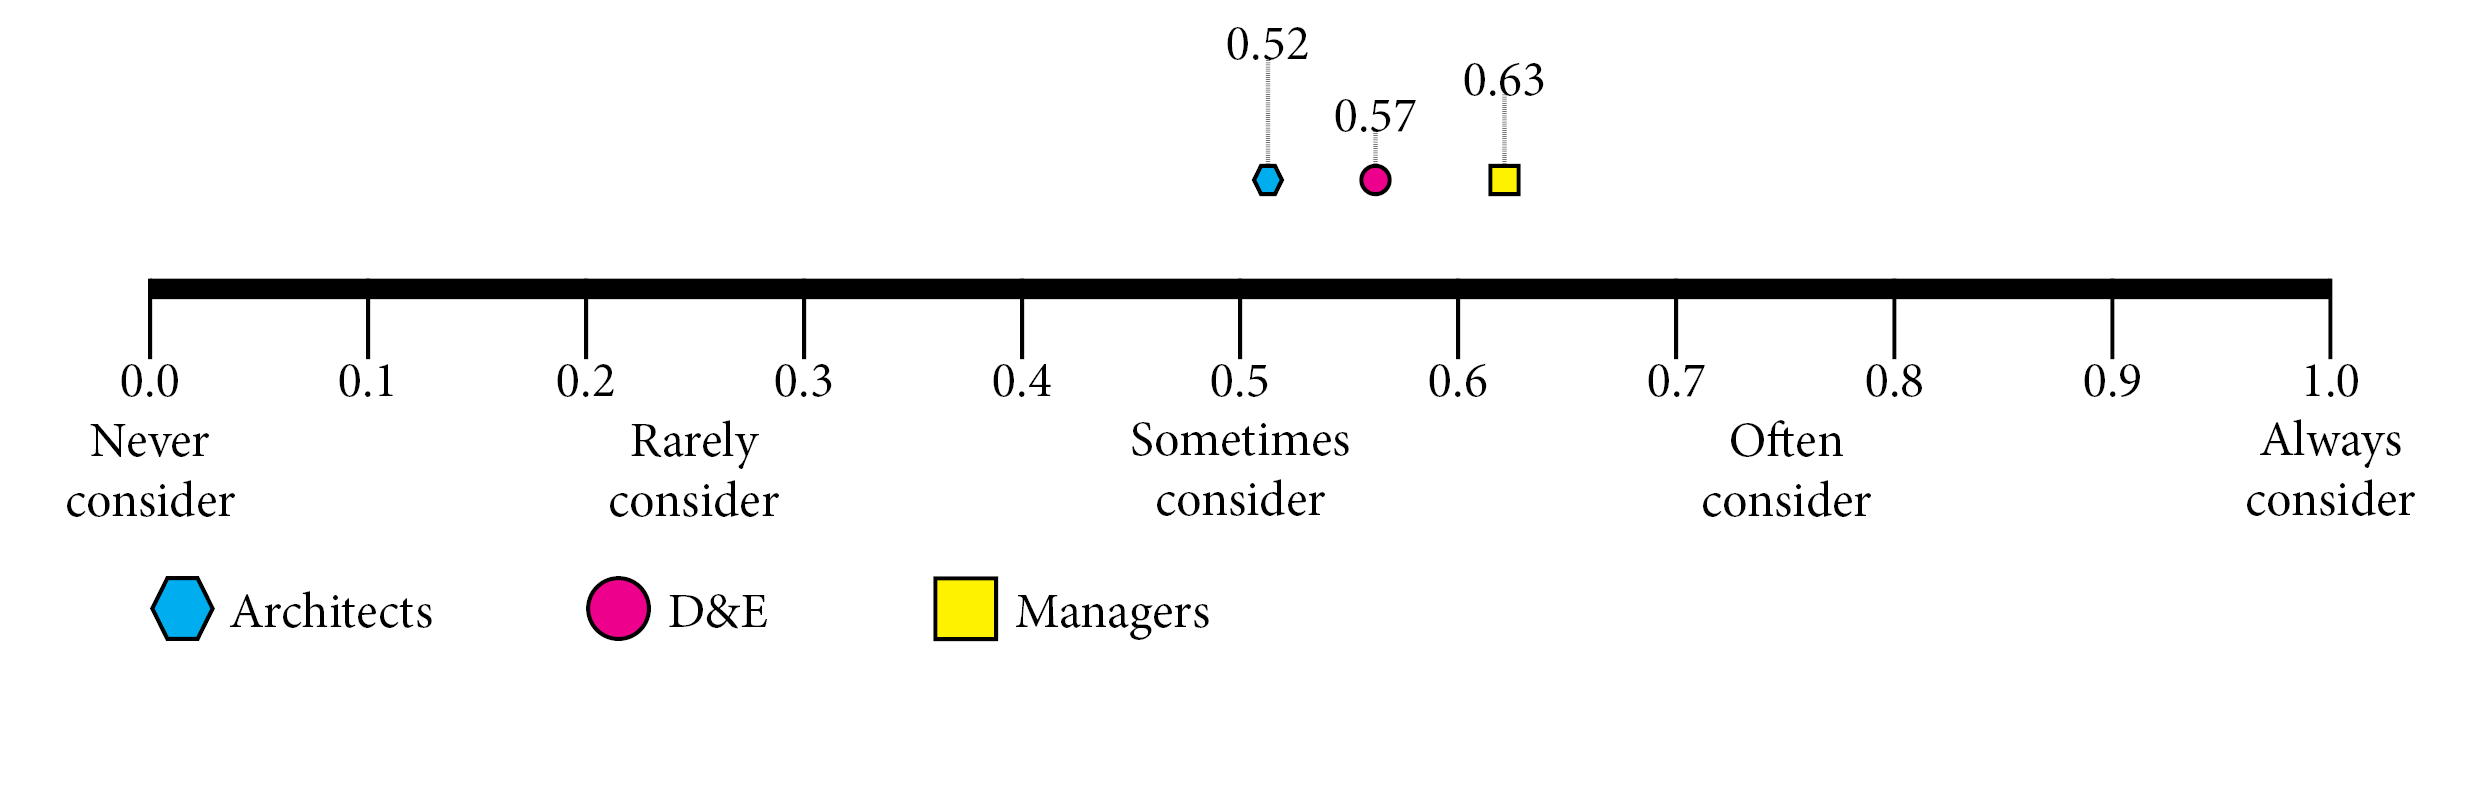
\includegraphics[width=\linewidth]{scorelines/aspect1.png}
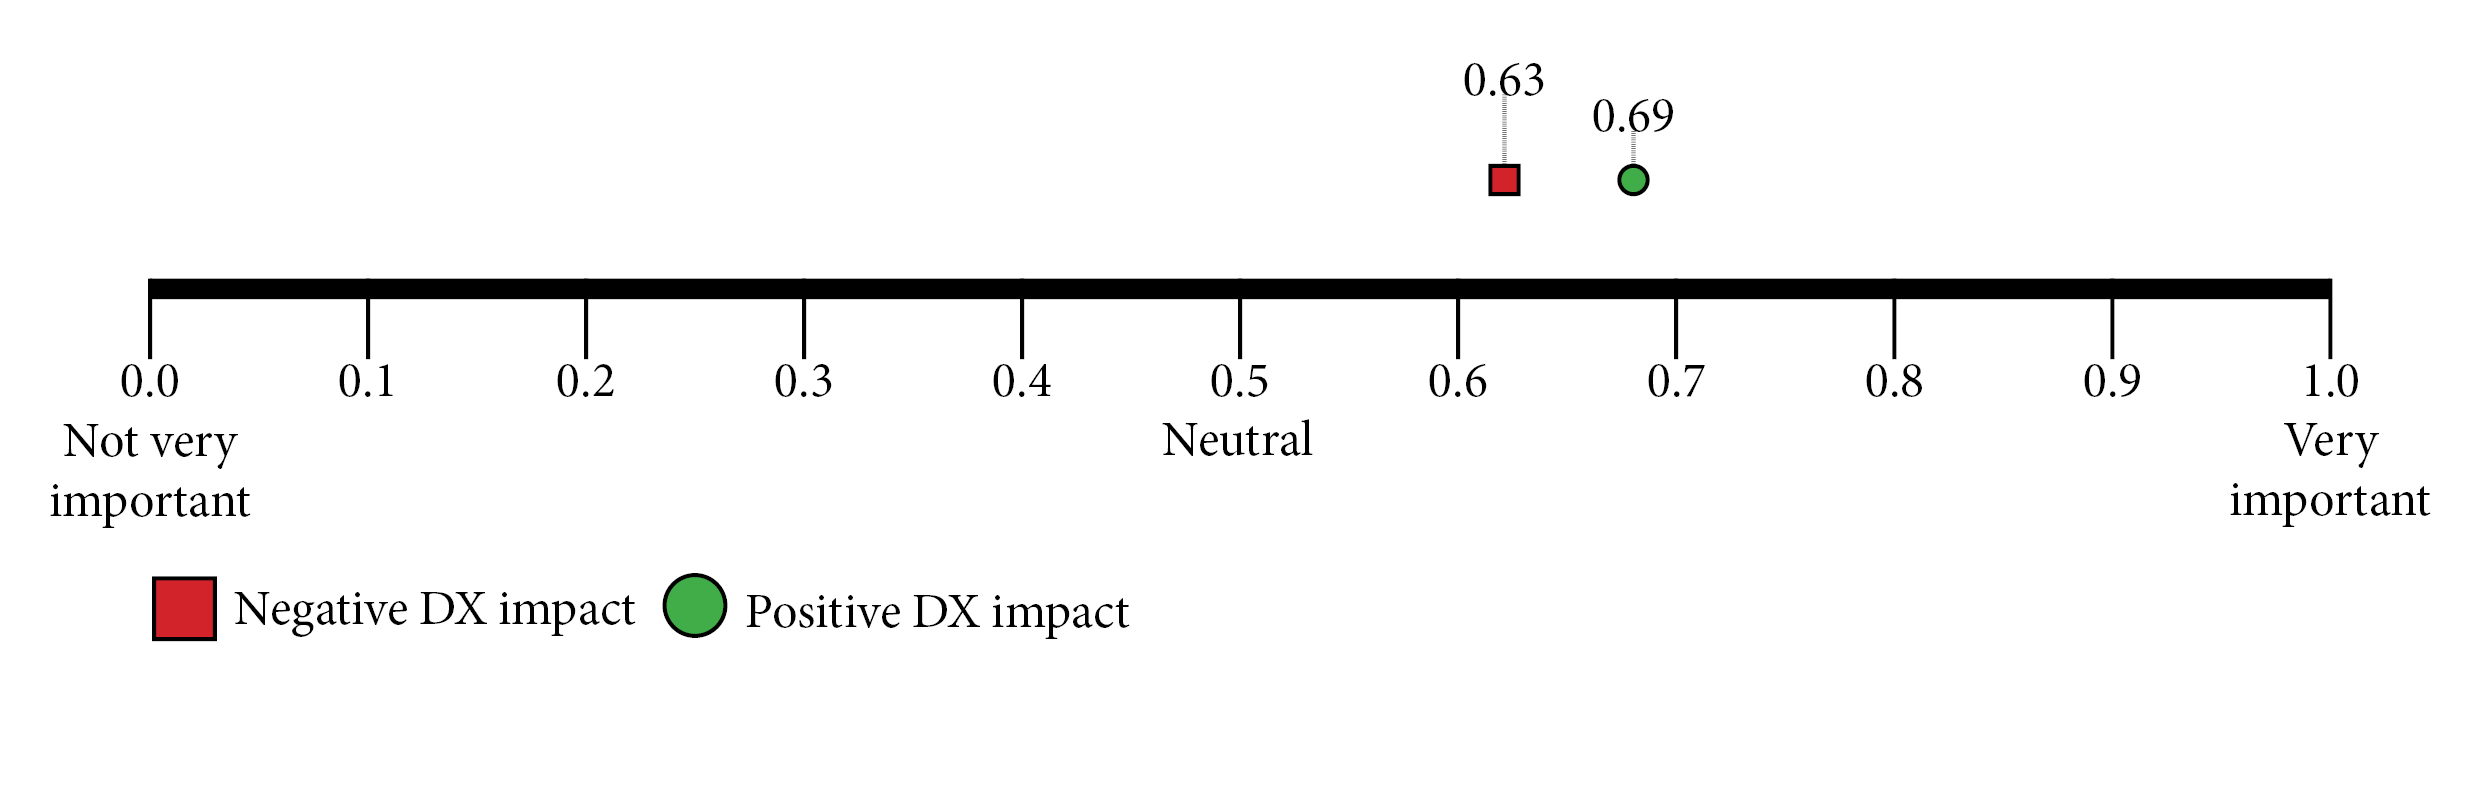
\includegraphics[width=\linewidth]{dxscorelines/dxaspect1.png}
\caption{Scoring for "How often the software is updated"}
\label{fig:aspect1}
\end{figure}
Updating of the software platform is of course important. Bugs need to be fixed, the compatibility for different platforms improved and new features might be added from time to time. In figure \ref{fig:aspect1} we can see how it's ranked. As we can see it's ranking somewhere in the middle. We also see that the DX impact is bigger than the consideration. As mentioned in section \ref{consisQuestions}, the DX-question and consideration question differed quite a bit, and we should careful to correlate these two. The DX impact shows however that being quick to address bugs has a bigger impact than the negative impact of being slow to address bugs.\\ \\The interviews showed that how often the software is updated can be seen as an indicator for how mature the software platform is. Too often and it will scare people away, as it's an indicator that there is a lot of bugs or the software is mature. If the software is updated not often enough it's an indicator that the software platform feels abandoned or not prioritised. The recommendation is to plan your updates carefully, try to lump small updates together into bigger ones, as to not update too often. Exemptions from this is critical bug fixes, such as relating to security or breaking bugs. To make this kind of planning is not a big effort, and therefor worth it. With the average score of 0.58/1.00 this aspect needs to be kept in mind, but not central. If you cater to managers, this aspect needs to kept more in mind. \\ \\
\textbf{Verdict: Somewhat important, but keep in mind. Medium effort, medium payoff.}
\subsubsection{I can have working code quickly}
\begin{figure}[H]
\centering
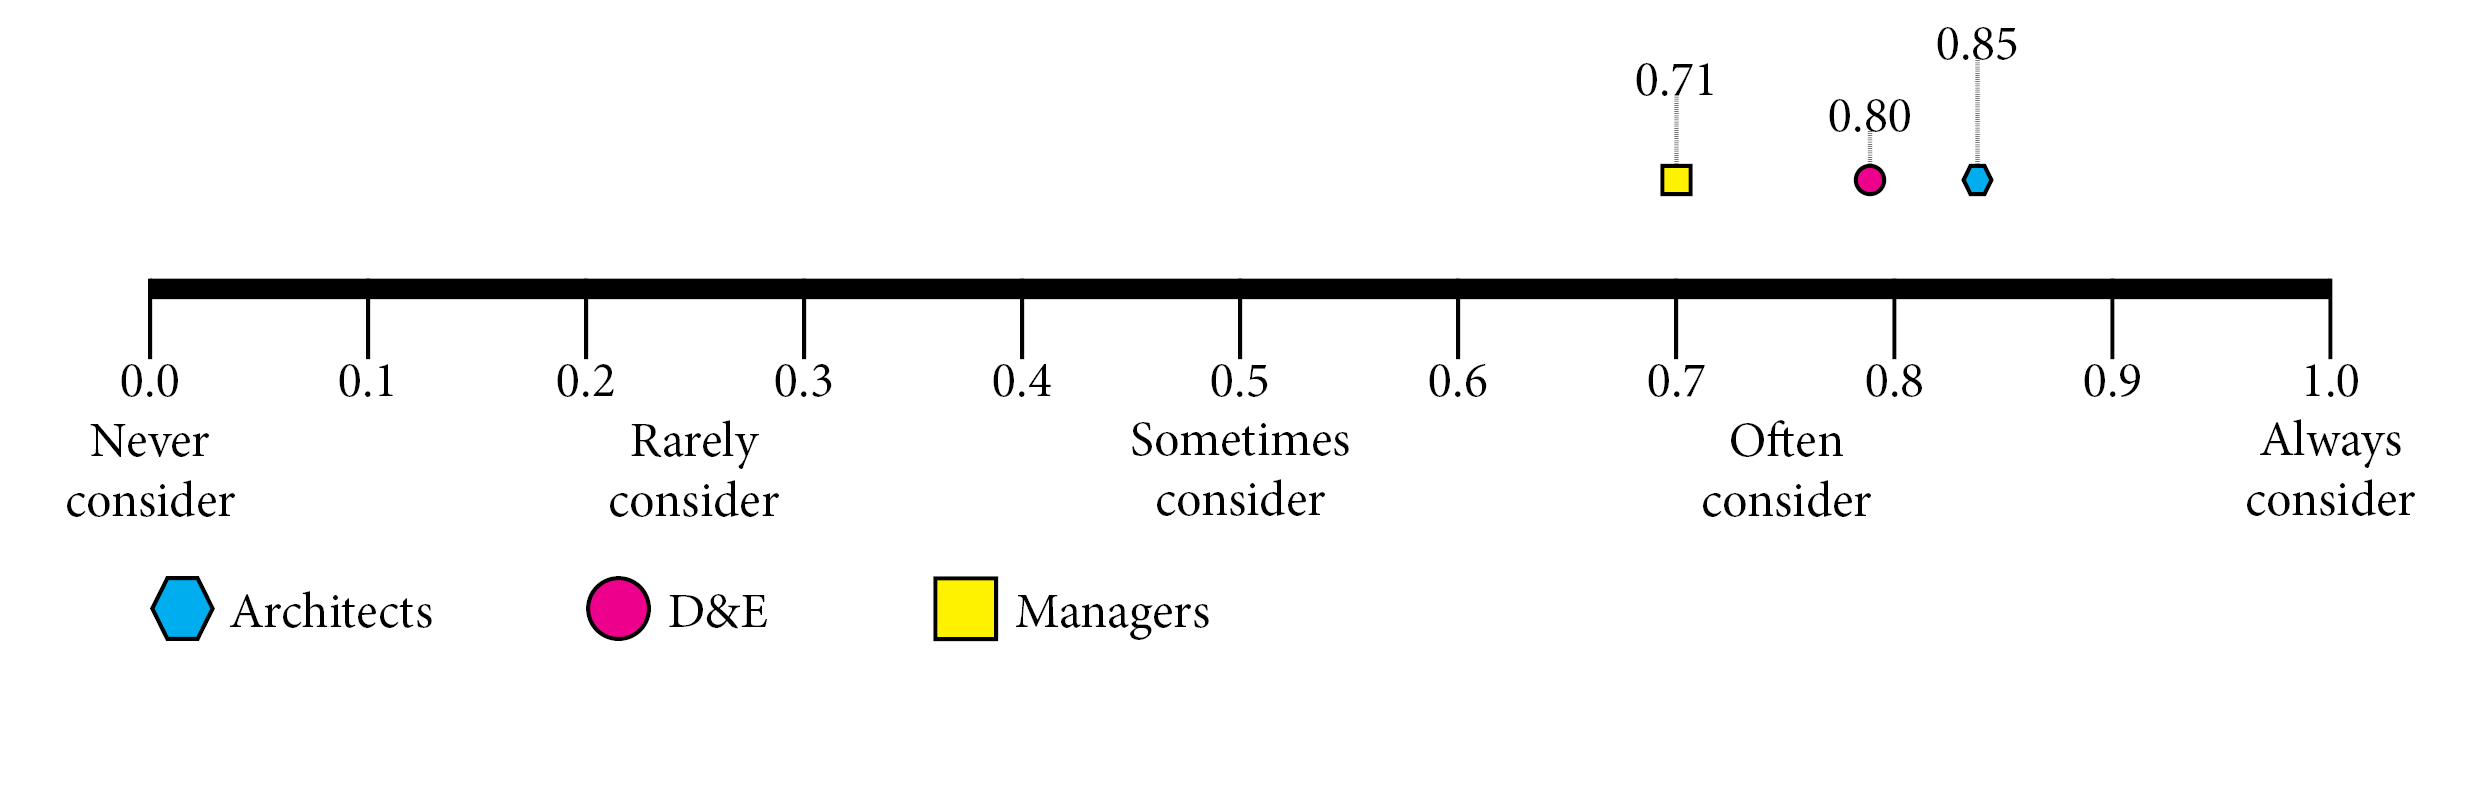
\includegraphics[width=\linewidth]{scorelines/aspect2.png}
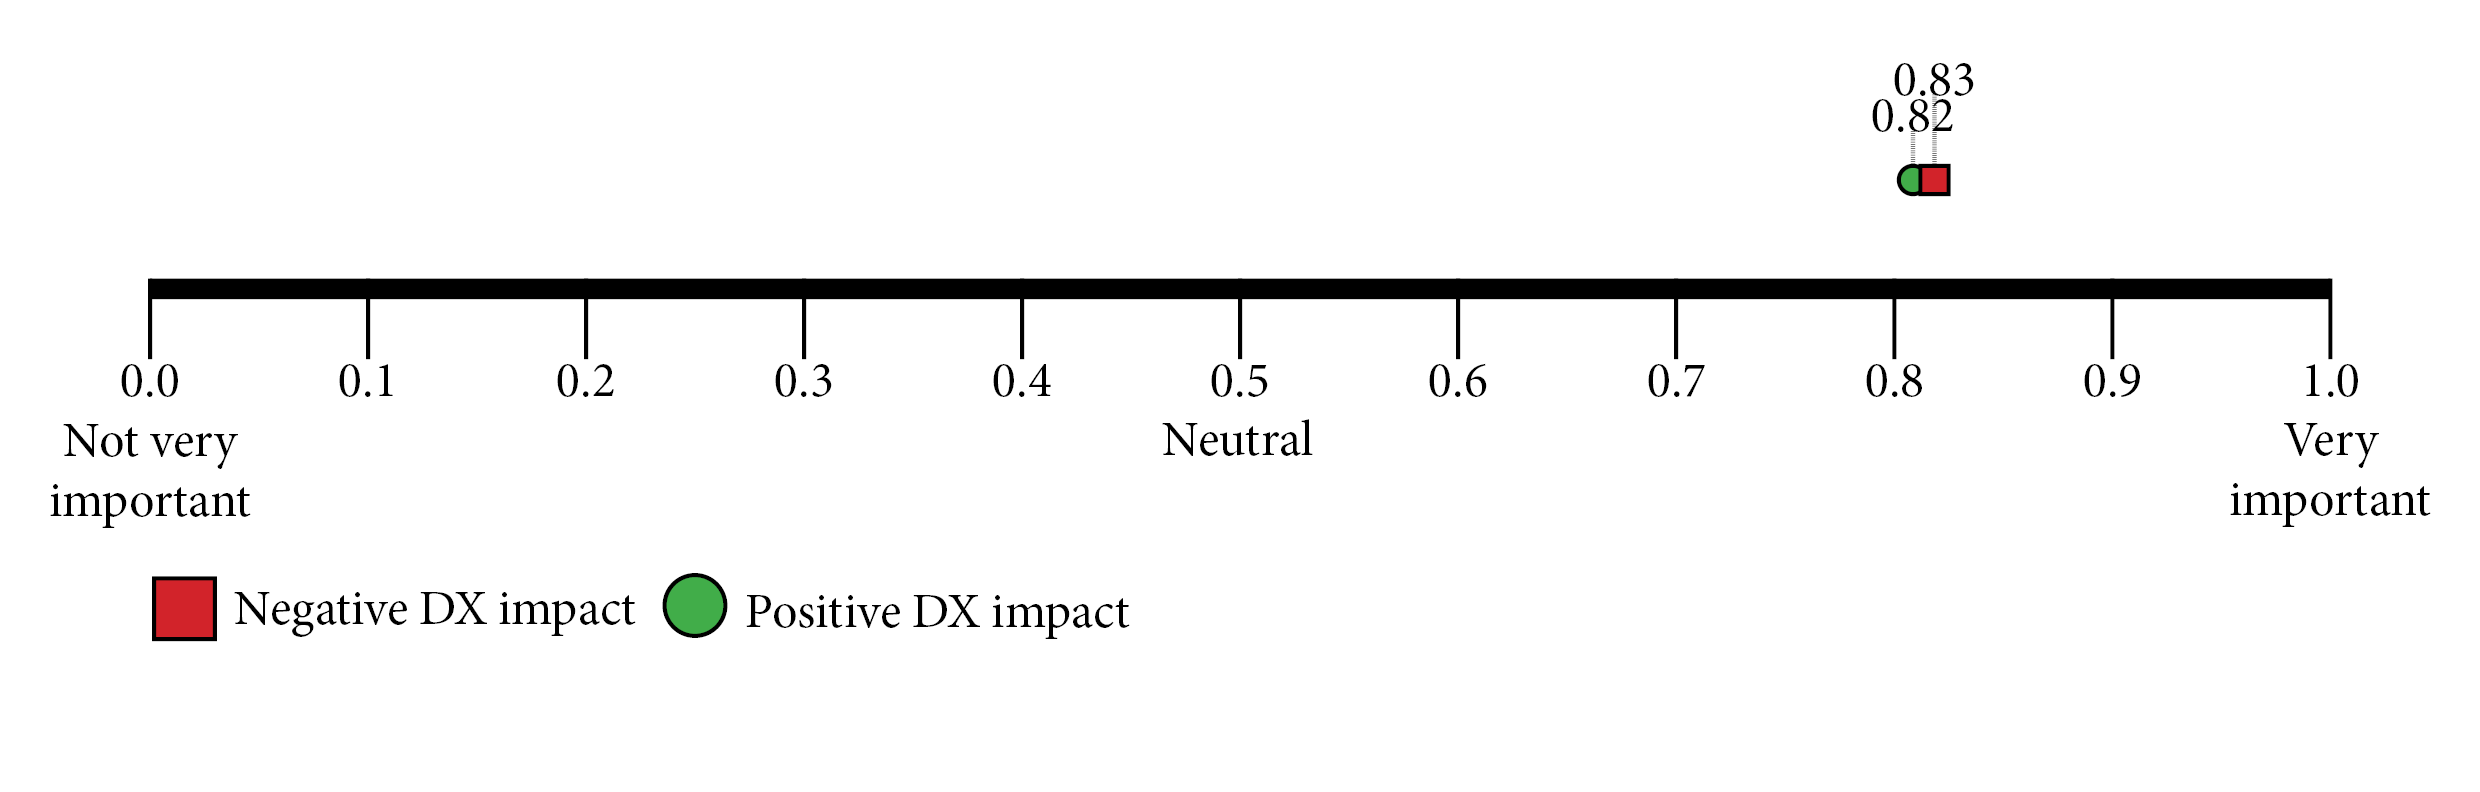
\includegraphics[width=\linewidth]{dxscorelines/dxaspect2.png}
\caption{Scoring for "I can have working code quickly"}
\label{fig:aspect2}
\end{figure}
Working code quickly has been shown to be important to developers. In figure \ref{fig:aspect2} we can see the scoring. With an average score of 0.80/1.00 this is an important aspect that should always be considered when creating a software platform. We also see that it has a strong DX impact. Not only are developers impatient people that want results quickly overall, working code quickly is developers way to figure out if a software platform is useful. Software developers quickly abandon software if they don't see it's value. Because working code quickly is their way of evaluating new software, it's extremely important to be able to provide this. The recommendation is to easily show how to get started. It should both be front and centre when you visit the website, and the example should be quick without being too simple. The effort to have an example that is easy to follow  and makes the user understand can take time, and be a bit of an effort, but is definitely worth it.\\ \\
\textbf{Very important, always keep in mind. Medium effort, high payoff.}
\subsubsection{The API documentation gives thorough explanations on how it works}
\begin{figure}[H]
\centering
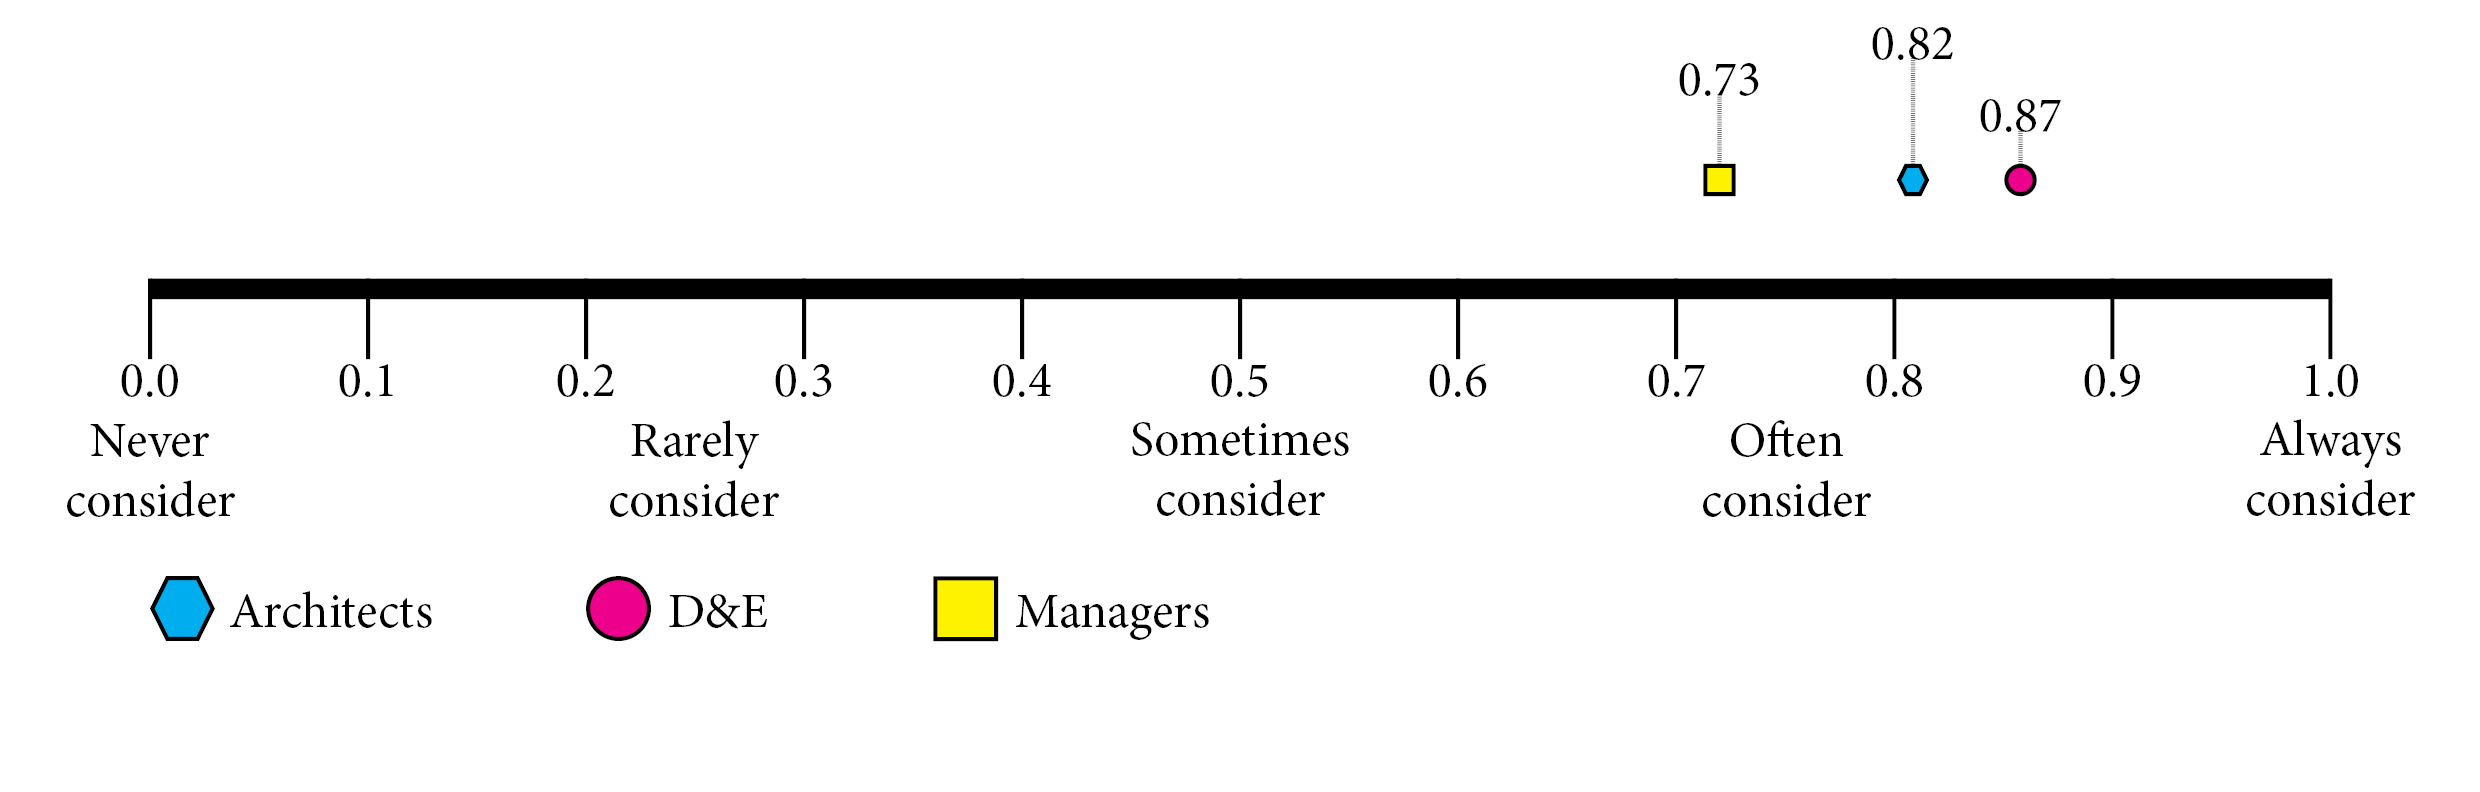
\includegraphics[width=\linewidth]{scorelines/aspect3.png}
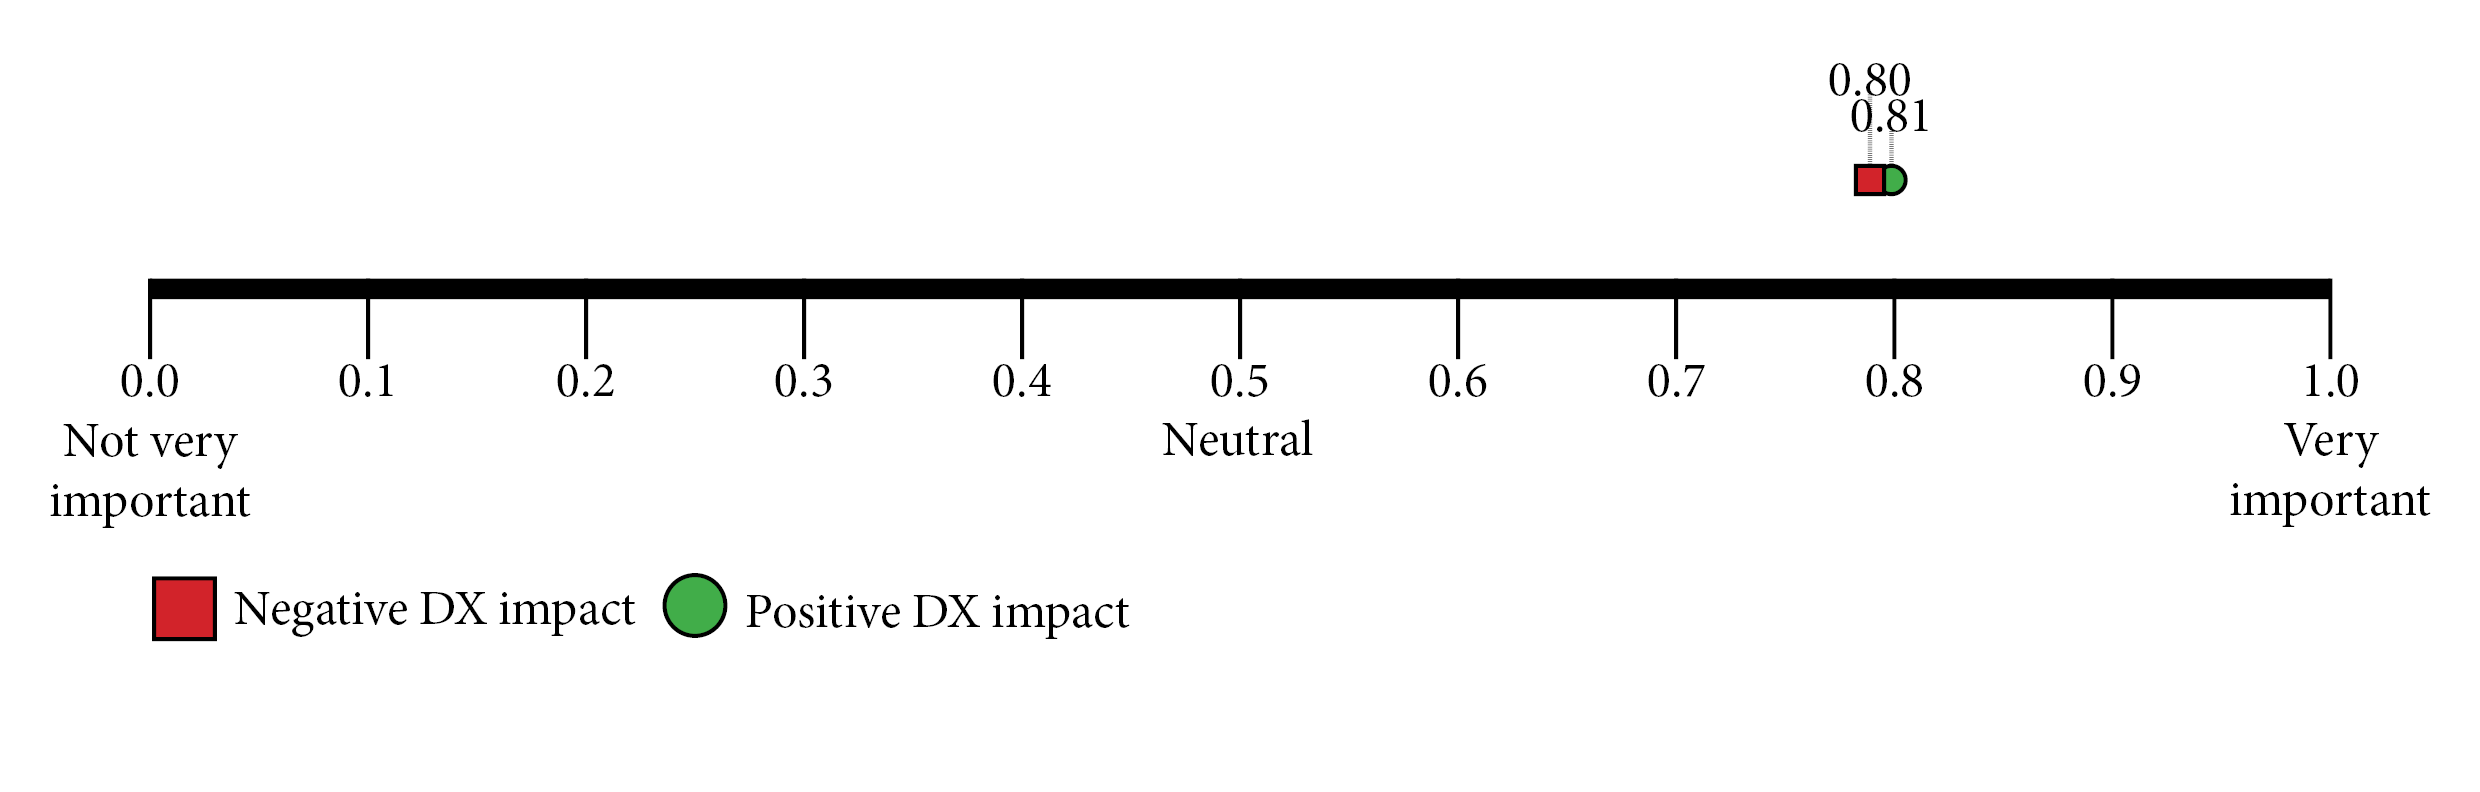
\includegraphics[width=\linewidth]{dxscorelines/dxaspect3.png}
\caption{Scoring for "The API documentation gives thorough explanations on how it works"}
\label{fig:aspect3}
\end{figure}
Documentation is the heart of a software platform, providing the explanation of how to use it. In figure \ref{fig:aspect3} we can see how it scored. With an average score of 0.82/1.00 it's paramount that this aspect is taken care of. This is also reflected in the DX impact result, where we see that poor documentation has a strong negative impact, and vice versa. Poor documentation was shown to cause developers to quickly abandon software. It doesn't matter how good your software platform is. If you don't have a good documentation that clearly explains how you're suppose to use it, people will not use your platform. You \textit{must} make sure you explain all parts of your platform. The effort to have thorough documentation is big, but is worth it when you see how important it is. The recommendation is to put a lot of effort into this, listen carefully to any questions you get from users. If a lot of users find the same things difficult, it can be an indicator that the documentation isn't thorough enough. A good method could be to read online discussions, and see what people have difficulty with.\\ \\
\textbf{Verdict: Very important, always keep in mind. High effort, high payoff.}
\subsubsection{The API has code examples}
\begin{figure}[H]
\centering
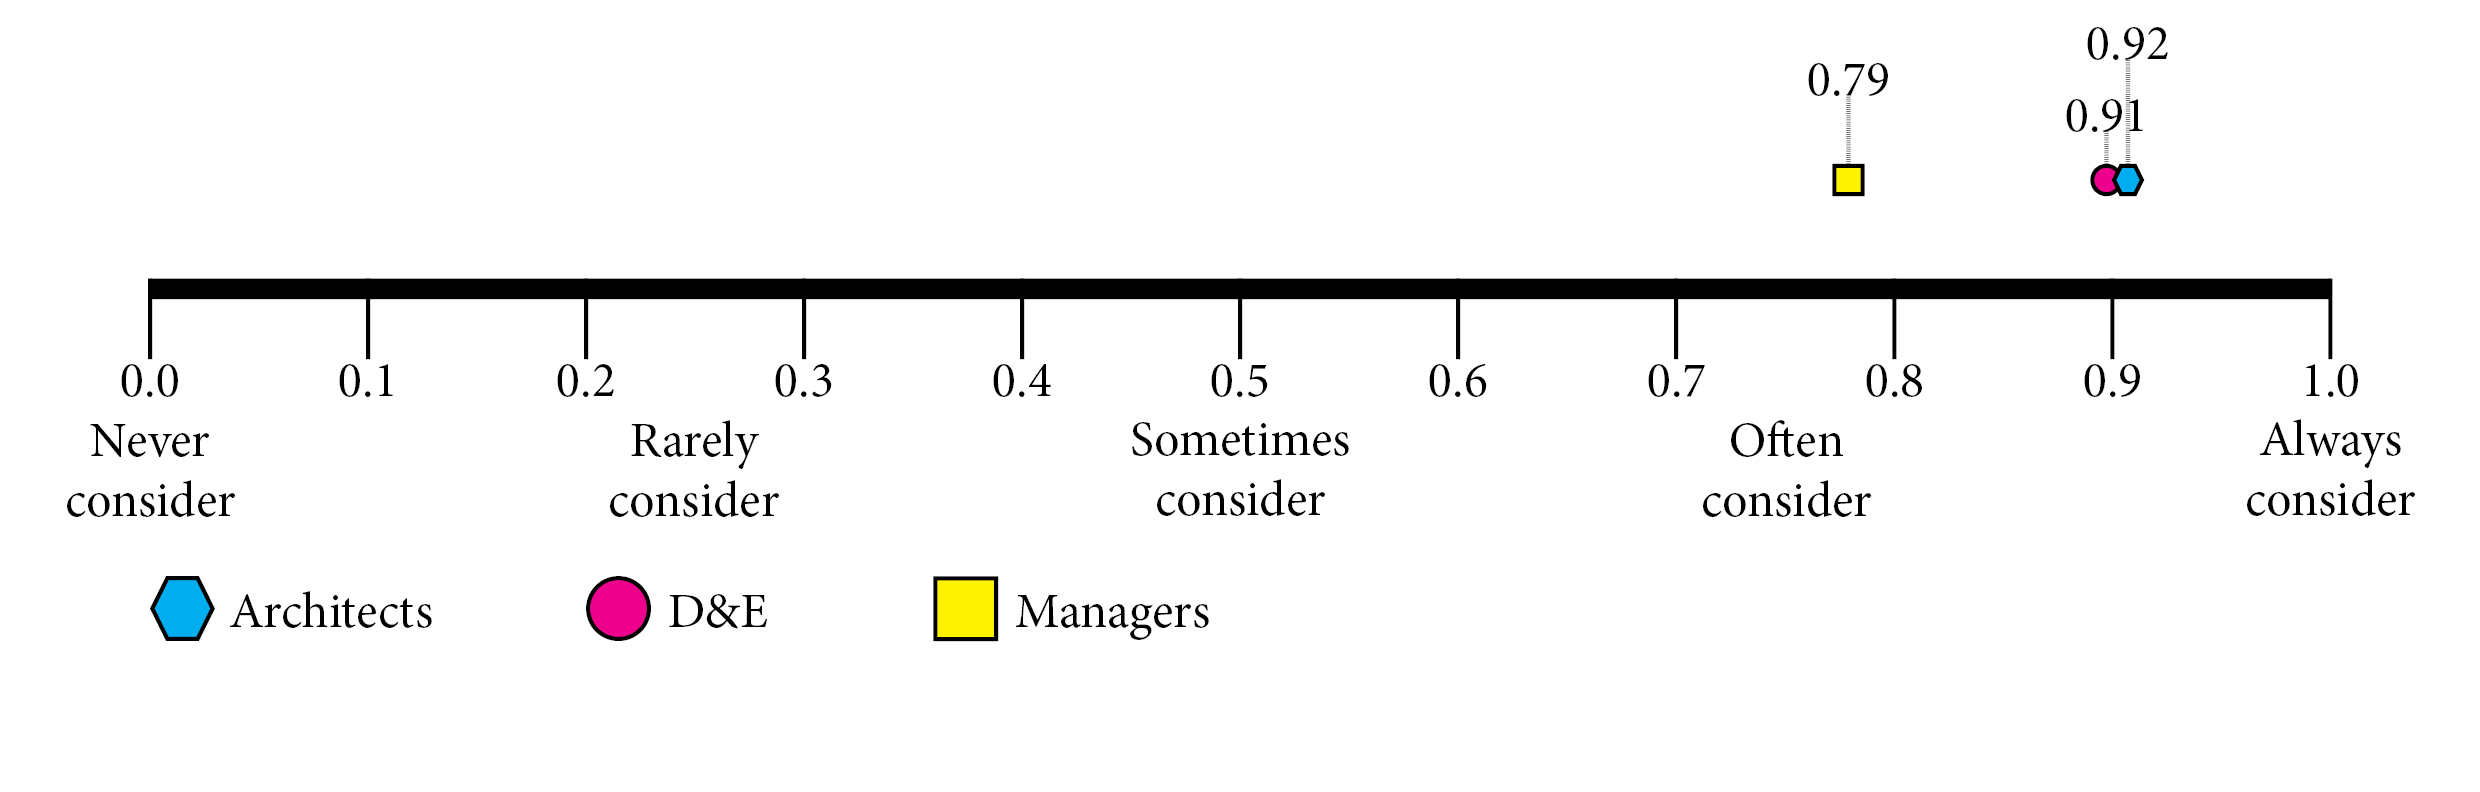
\includegraphics[width=\linewidth]{scorelines/aspect4.png}
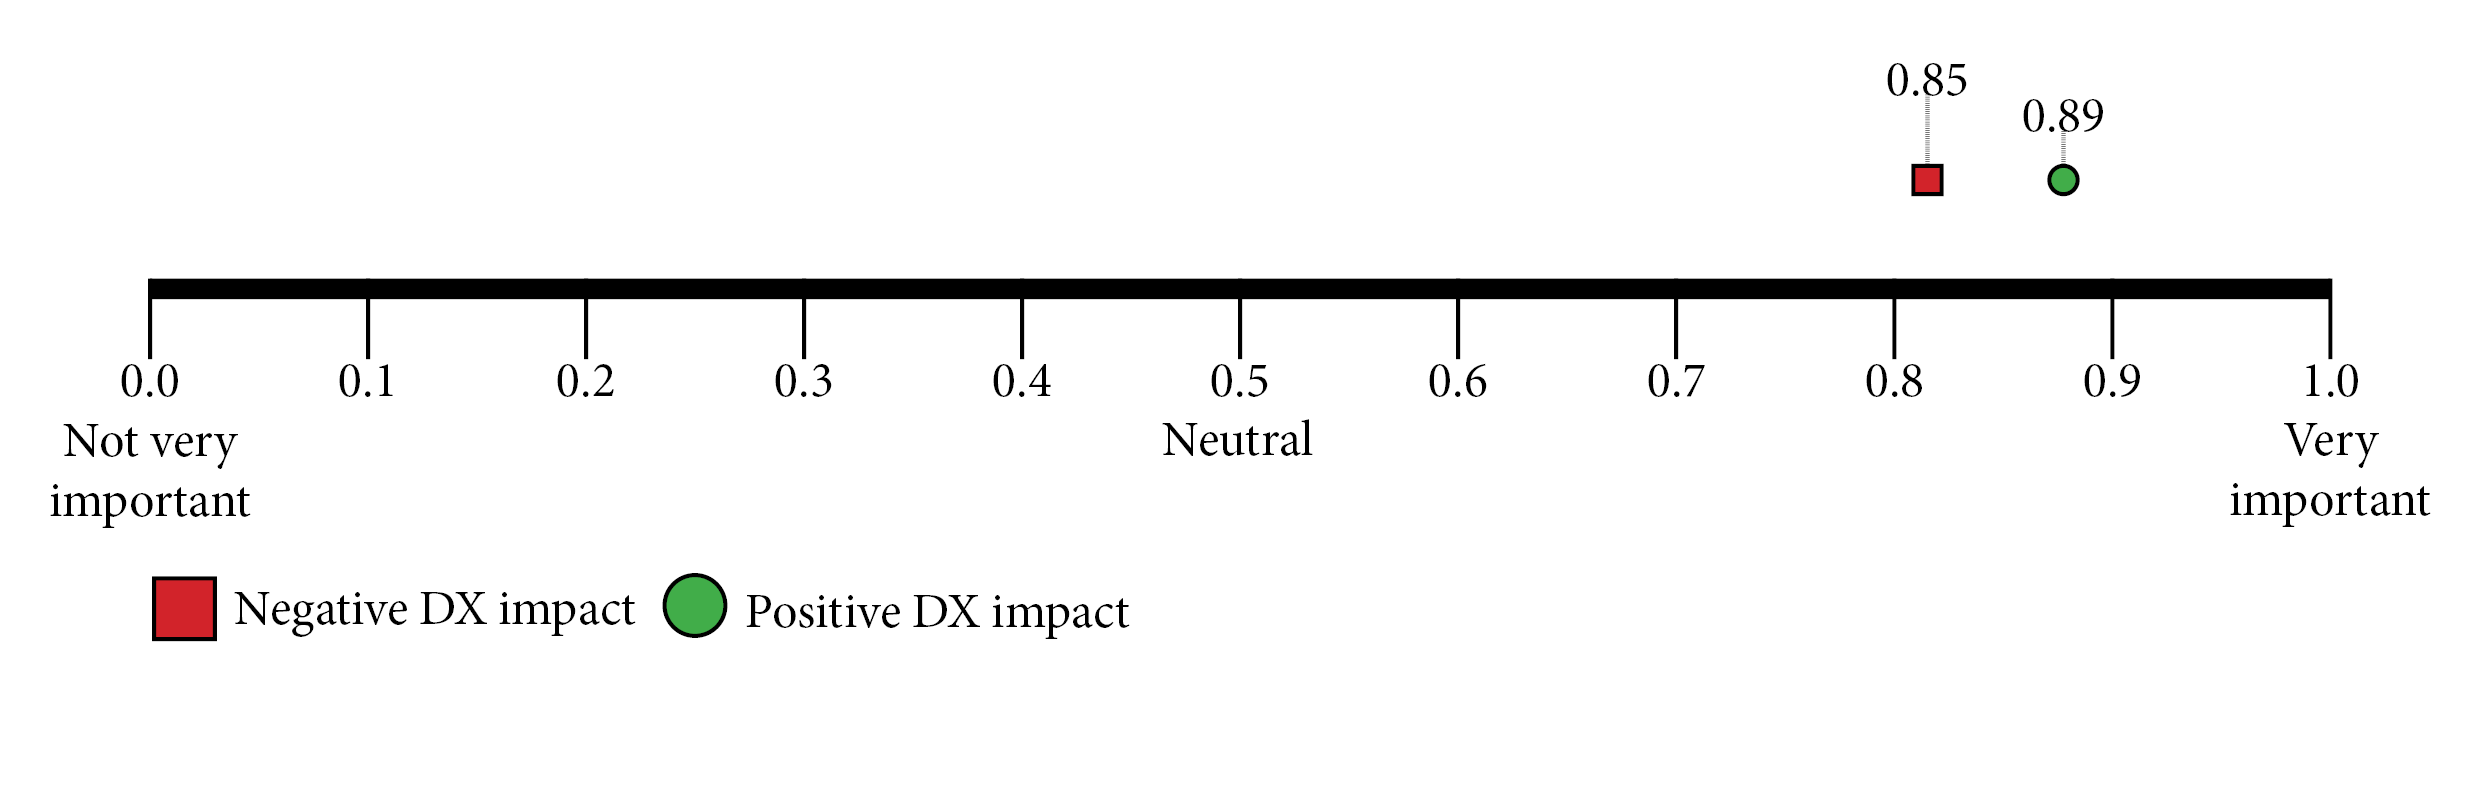
\includegraphics[width=\linewidth]{dxscorelines/dxaspect4.png}
\caption{Scoring for "The API has code examples"}
\label{fig:aspect4}
\end{figure}
You can explain concepts and methods in text, but often an example is the best way to convey something quickly. The interviews showed that examples is the first thing people look at when encountering documentation. It is therefor important that the example is front and centre in documentation. The examples are used for many things too. It's for copy-pasting into people's projects, getting an overview how things work and are linked together as well as to simply see how things should be used. The effort to construct good examples is quite high. The recommendation is to \texit{always} have a simple example with all methods and concepts, and if possible more advanced examples too. The simple example should be concise, and show the standard situation. It could be tempting to show something fancy. This however increases the risk for confusion. If you're going to show advanced situations, do it in step-by-steps as to not confuse the user. In figure \ref{fig:aspect4} you can see how it scored. With an average score of 0.90/1.00 and a strong DX impact it's paramount that this aspect is taken care of. It's the first thing users look at, and if they don't understand you risk losing them. \\ \\
\textbf{Very important, always keep in mind. High effort, high payoff.}
\subsubsection{The documentation doesn’t assume any prior expertise}
\begin{figure}[H]
\centering
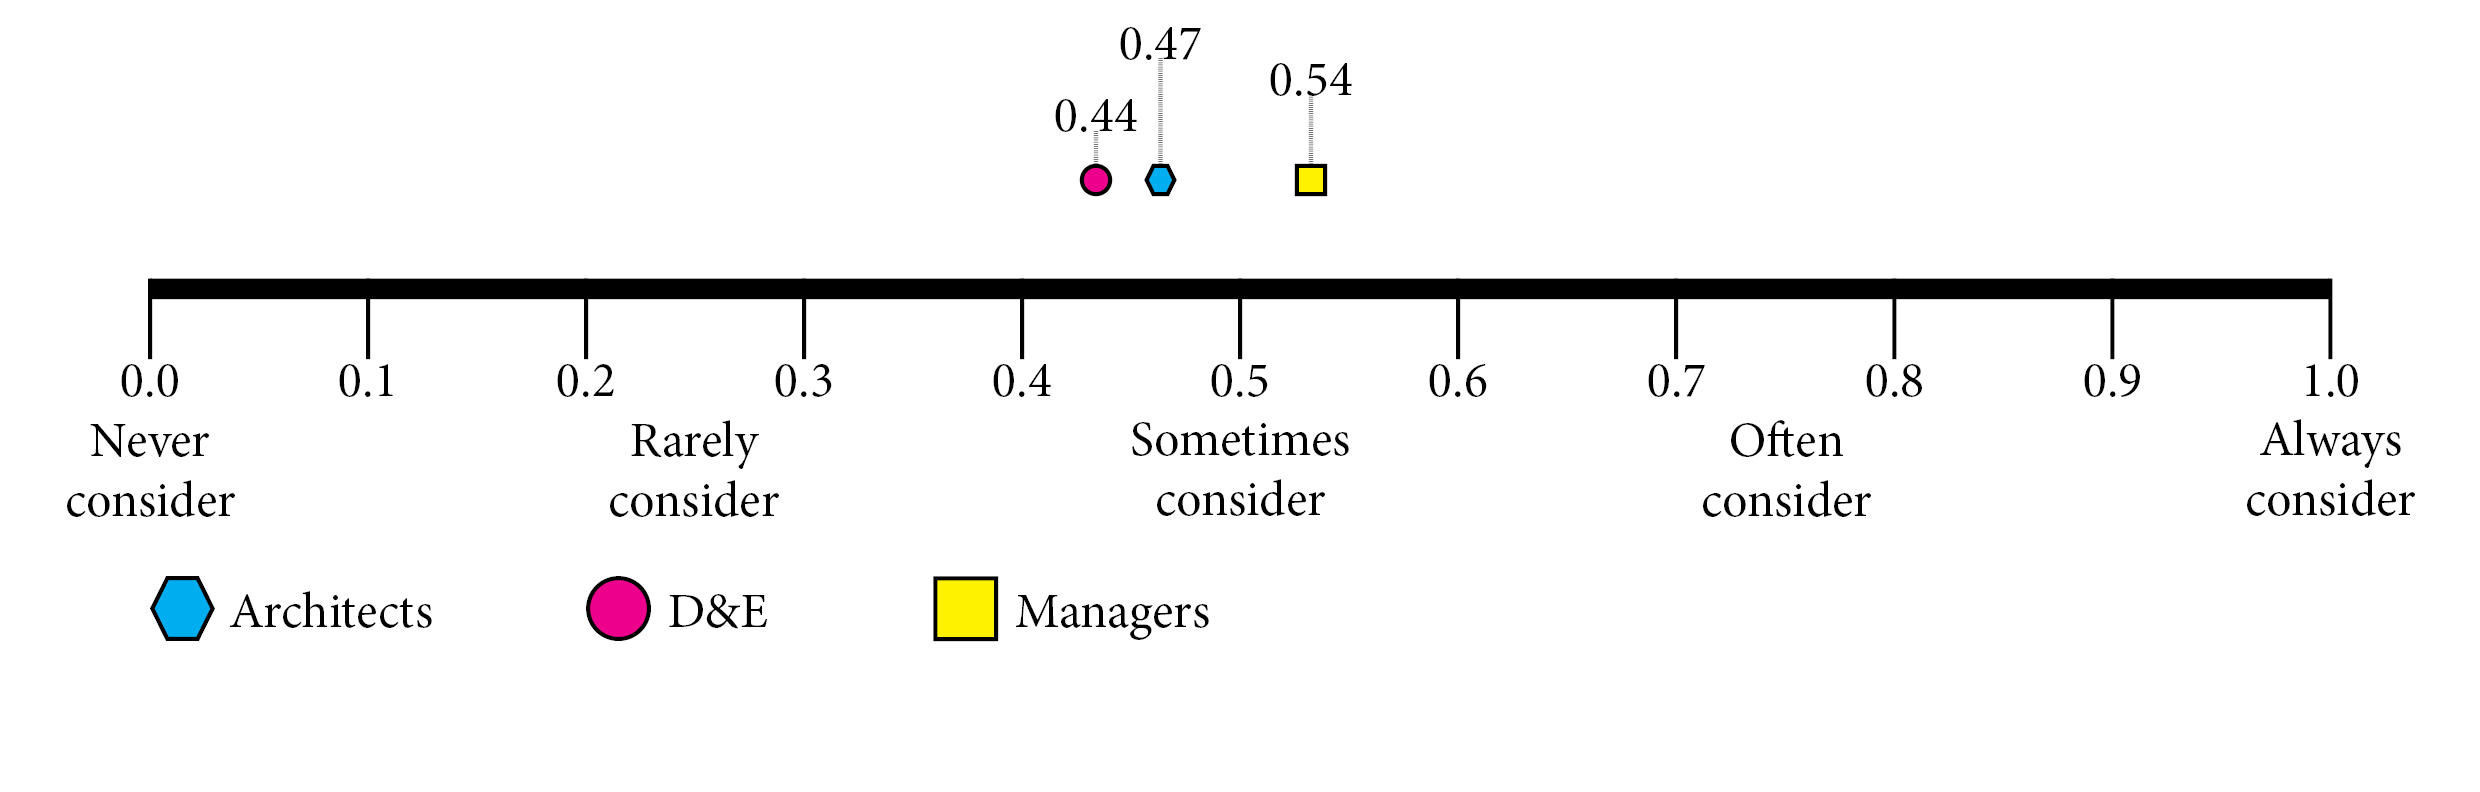
\includegraphics[width=\linewidth]{scorelines/aspect5.png}
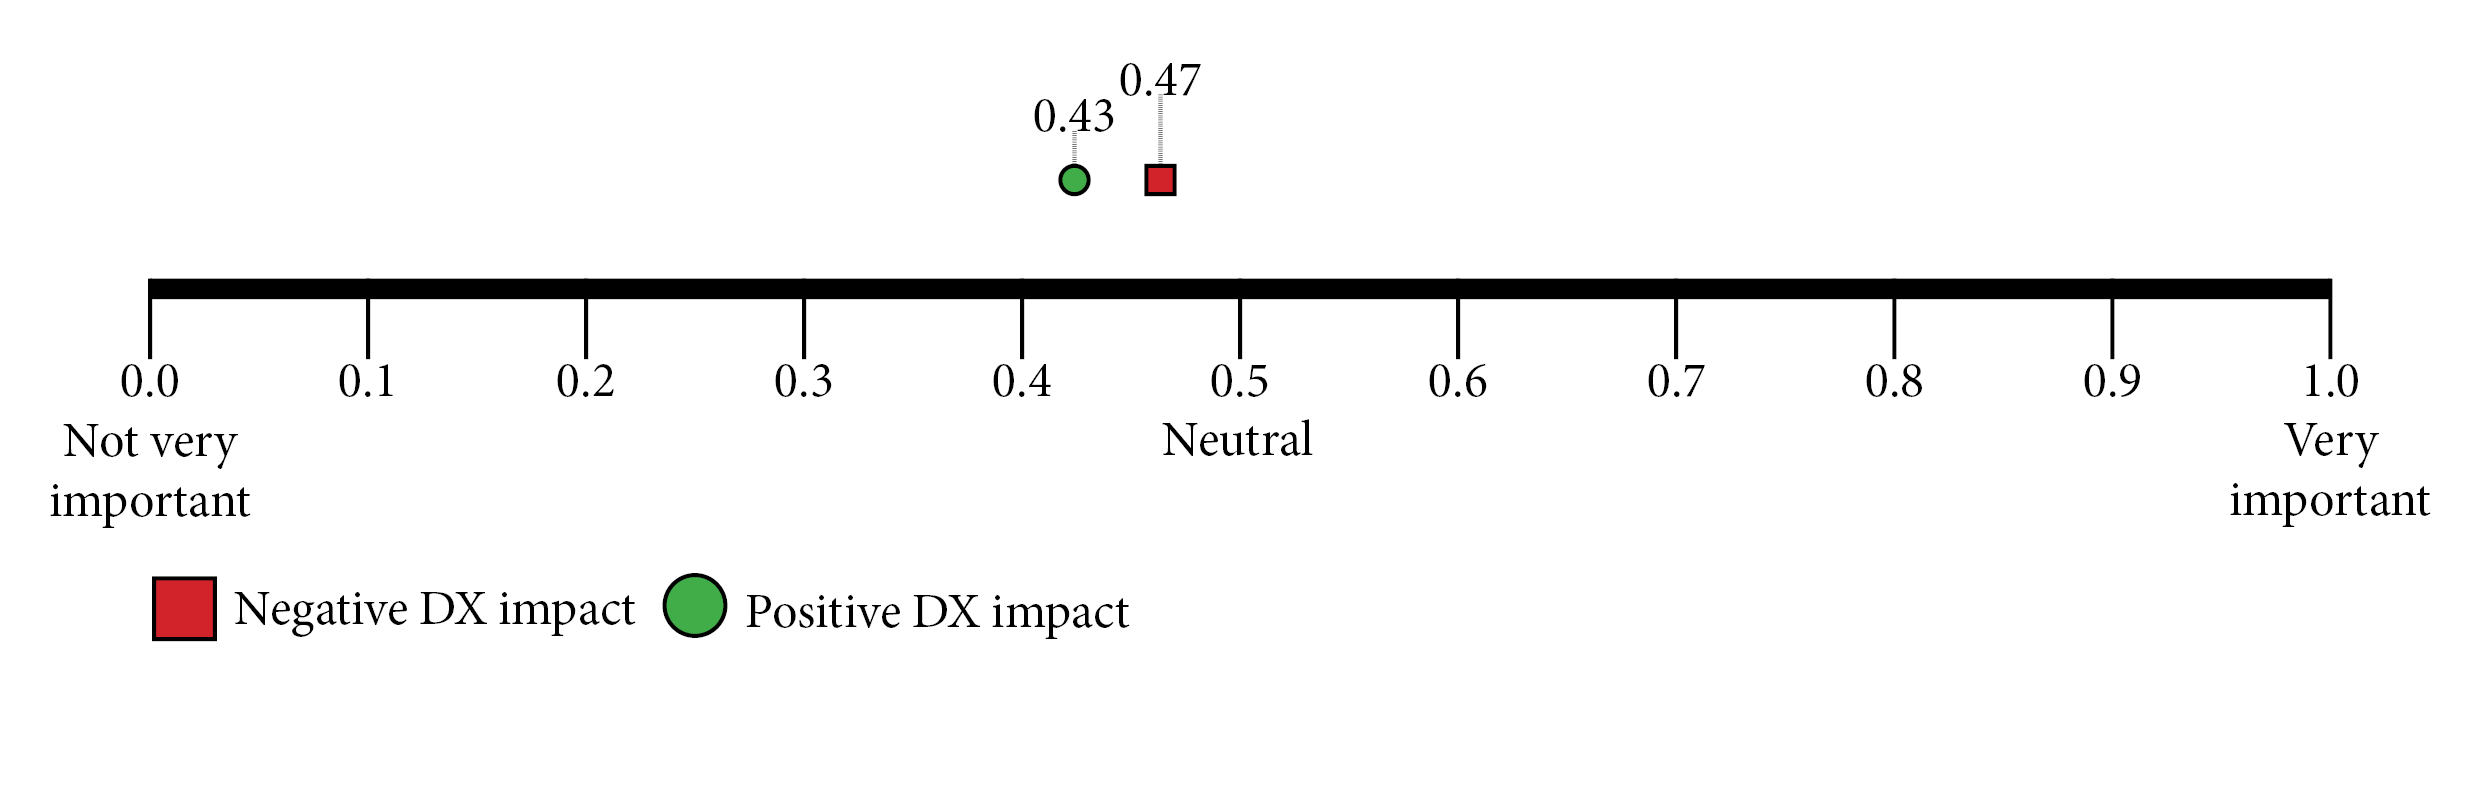
\includegraphics[width=\linewidth]{dxscorelines/dxaspect5.png}
\caption{Scoring for "The documentation doesn’t assume any prior expertise"}
\label{fig:aspect5}
\end{figure}
Software platforms will naturally have concepts that are new to people. Whenever a new concept is used, you risk confusing the user if it's not explained. In figure \ref{fig:aspect5} you can see that it does not score very high, with an average of 0.47/1.00. We also see that the DX impact scores about the same as the consideration questions. This doesn't mean that it can be completely ignored, but people are not scared away by new concepts. The recommendation is to link to an explanations of new concepts where ever they're used. This effort is not very big, but solves the problem. \\ \\
\textbf{Verdict: Not very important, but don't ignore. Low effort, medium payoff.}
\subsubsection{The documentation has consistent language}
\begin{figure}[H]
\centering
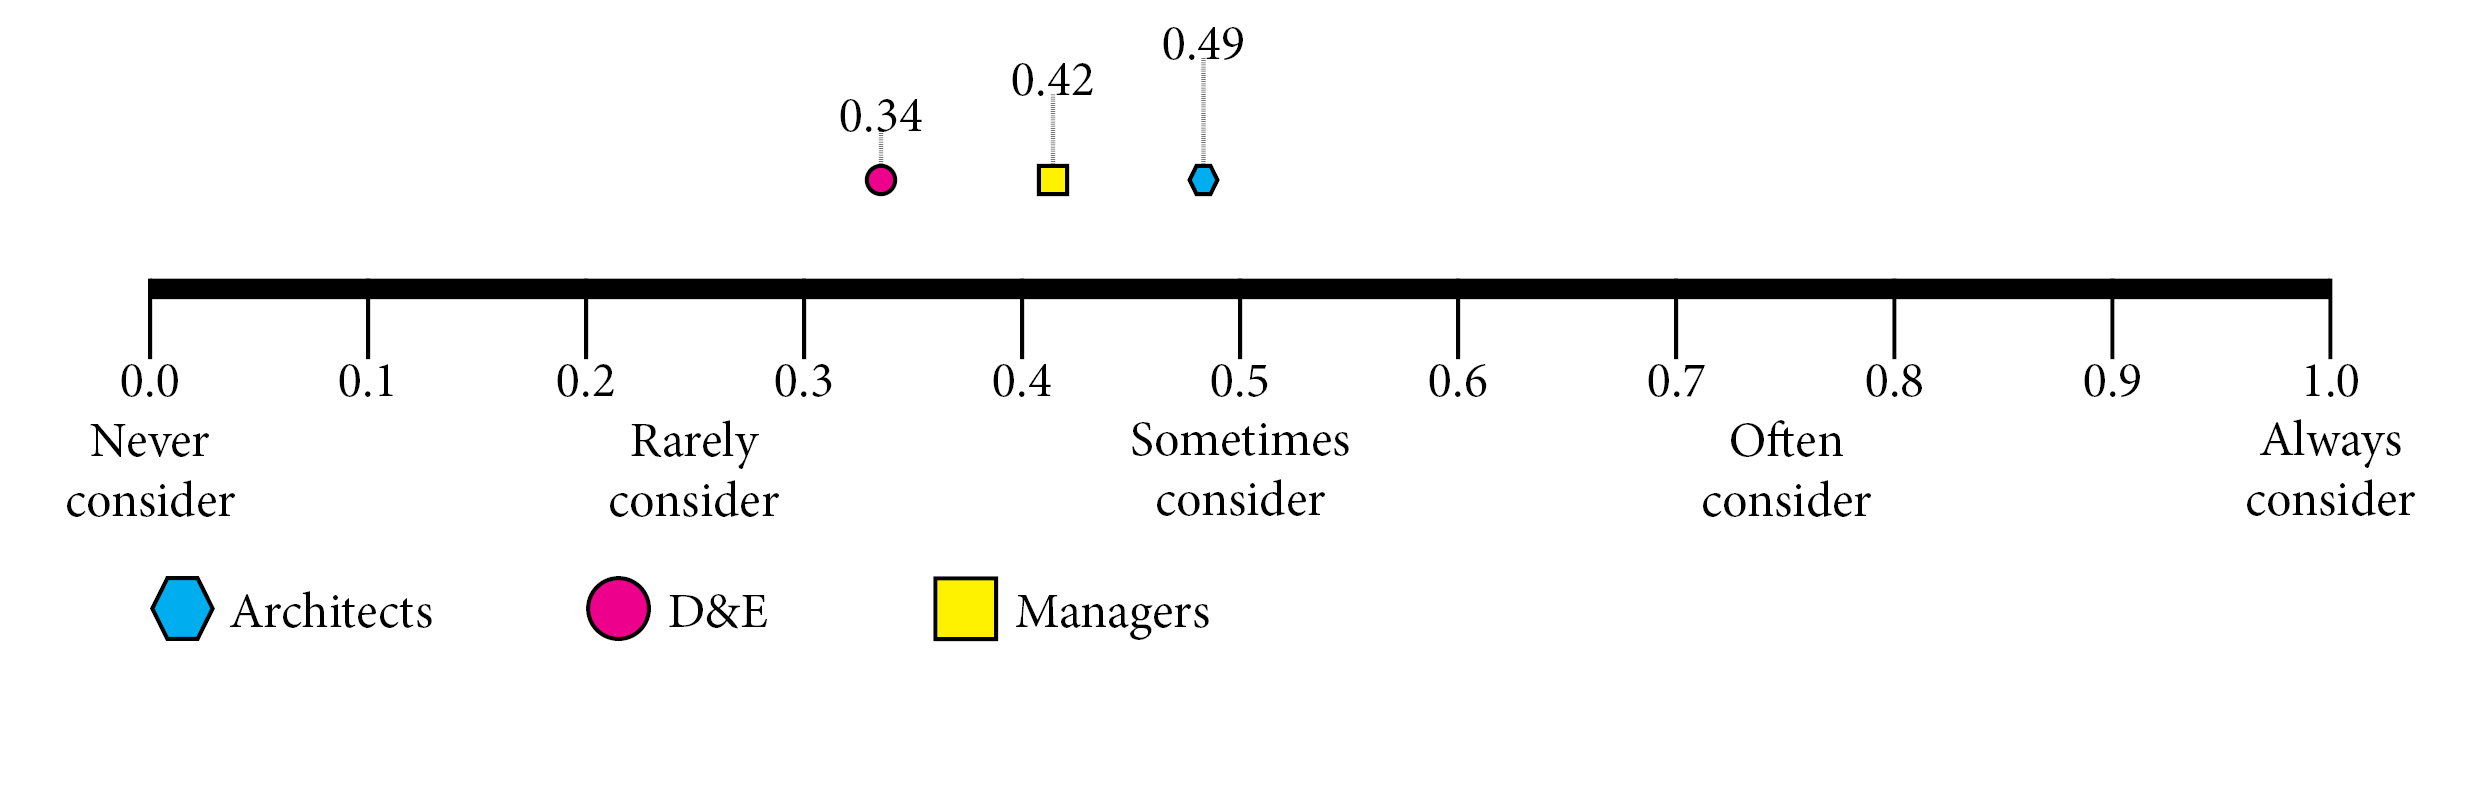
\includegraphics[width=\linewidth]{scorelines/aspect6.png}
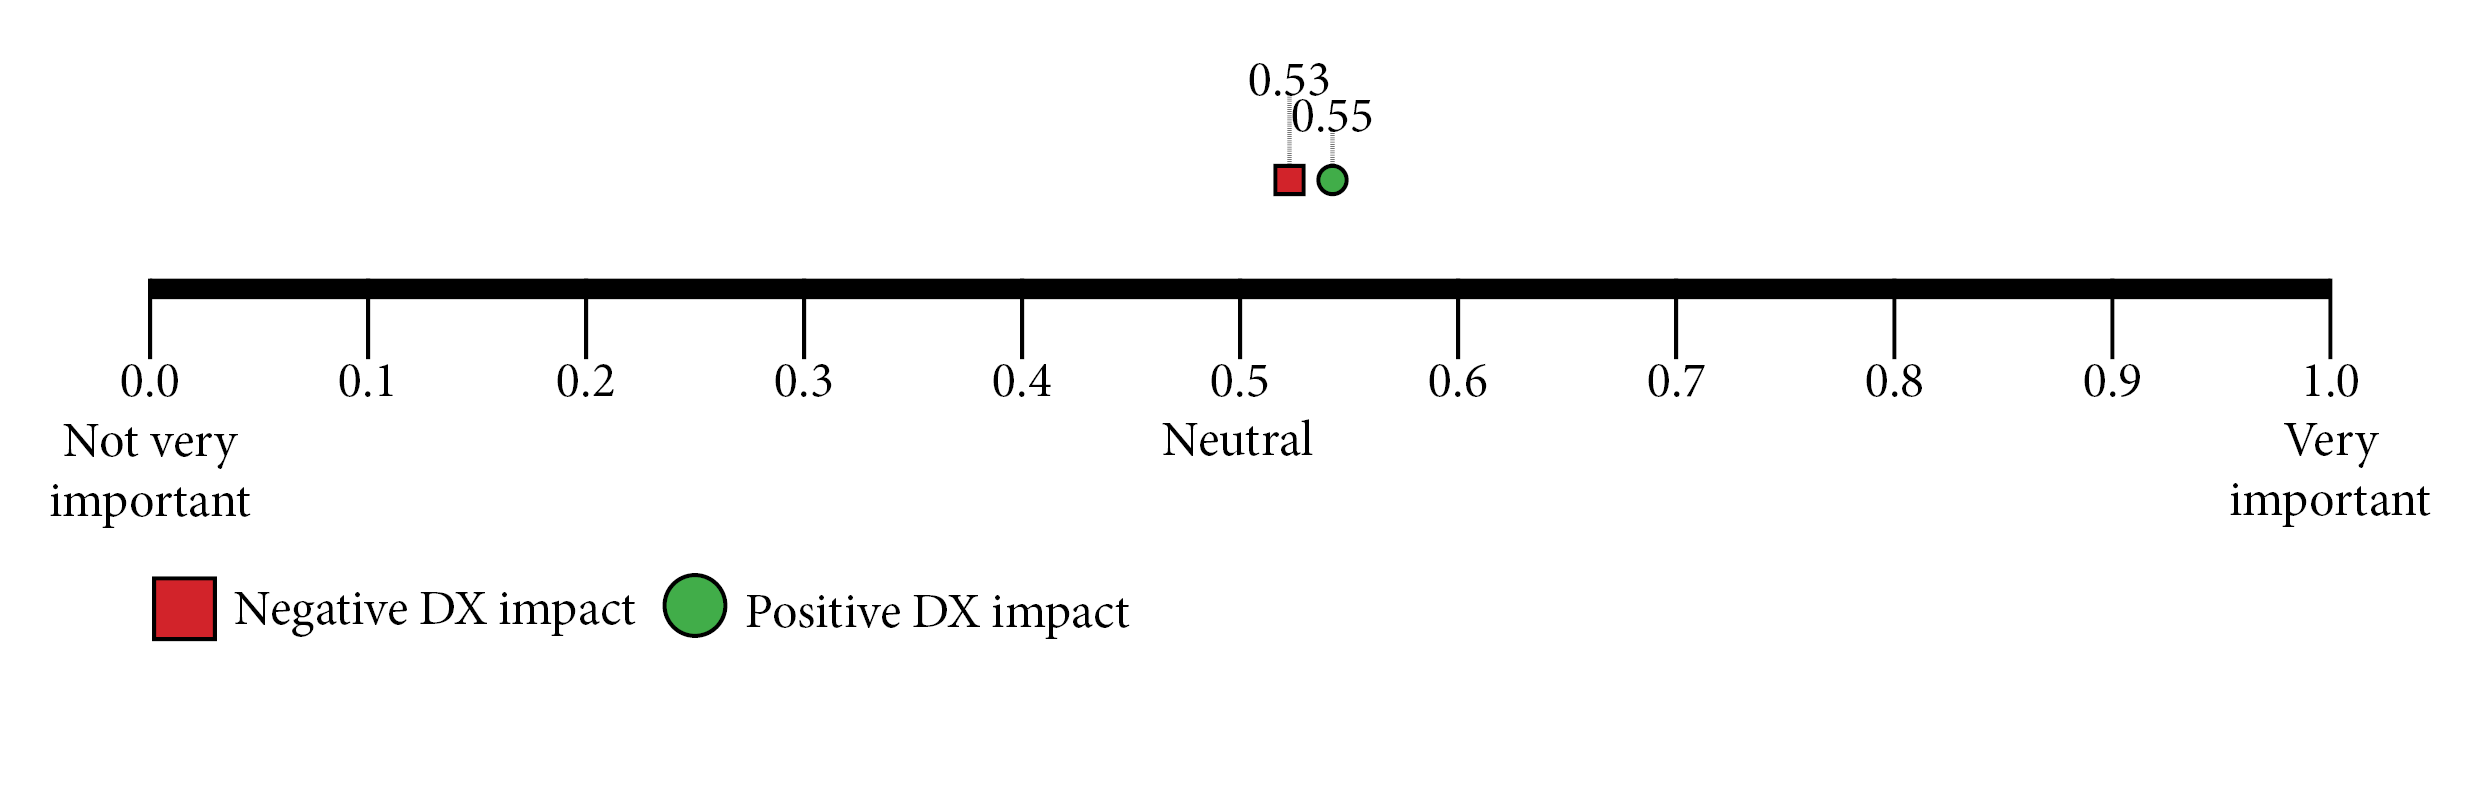
\includegraphics[width=\linewidth]{dxscorelines/dxaspect6.png}
\caption{Scoring for "The documentation has consistent language"}
\label{fig:aspect6}
\end{figure}
Having consistent language is an indicator of a documentation that has been thoroughly reviewed and worked with. In figure \ref{fig:aspect6} however we can see that it scores quite low, with an average of 0.41/1.00. We also see that although it's not quite often considered, it has a stronger DX impact. It's however still close to neutral. A documentation with inconsistency language is still very much usable, it just increases the risk for confusion. The effort to fix an already inconsistent documentation is very high. The recommendation is to define a vocabulary that should be used by the documentation writers before starting to write documentation, or from now on if the documentation has already been written. This will ensure that new documentation has consistency, as long as the documentation make sure to use the vocabulary. Because of the high effort, and low importance according to this research, going through documentation and fixing inconsistency should not be of very high priority.\\ \\
\textbf{Verdict: Not very important, but don't ignore. High effort, low payoff.}
\subsubsection{The documentation is easy to navigate}
\begin{figure}[H]
\centering
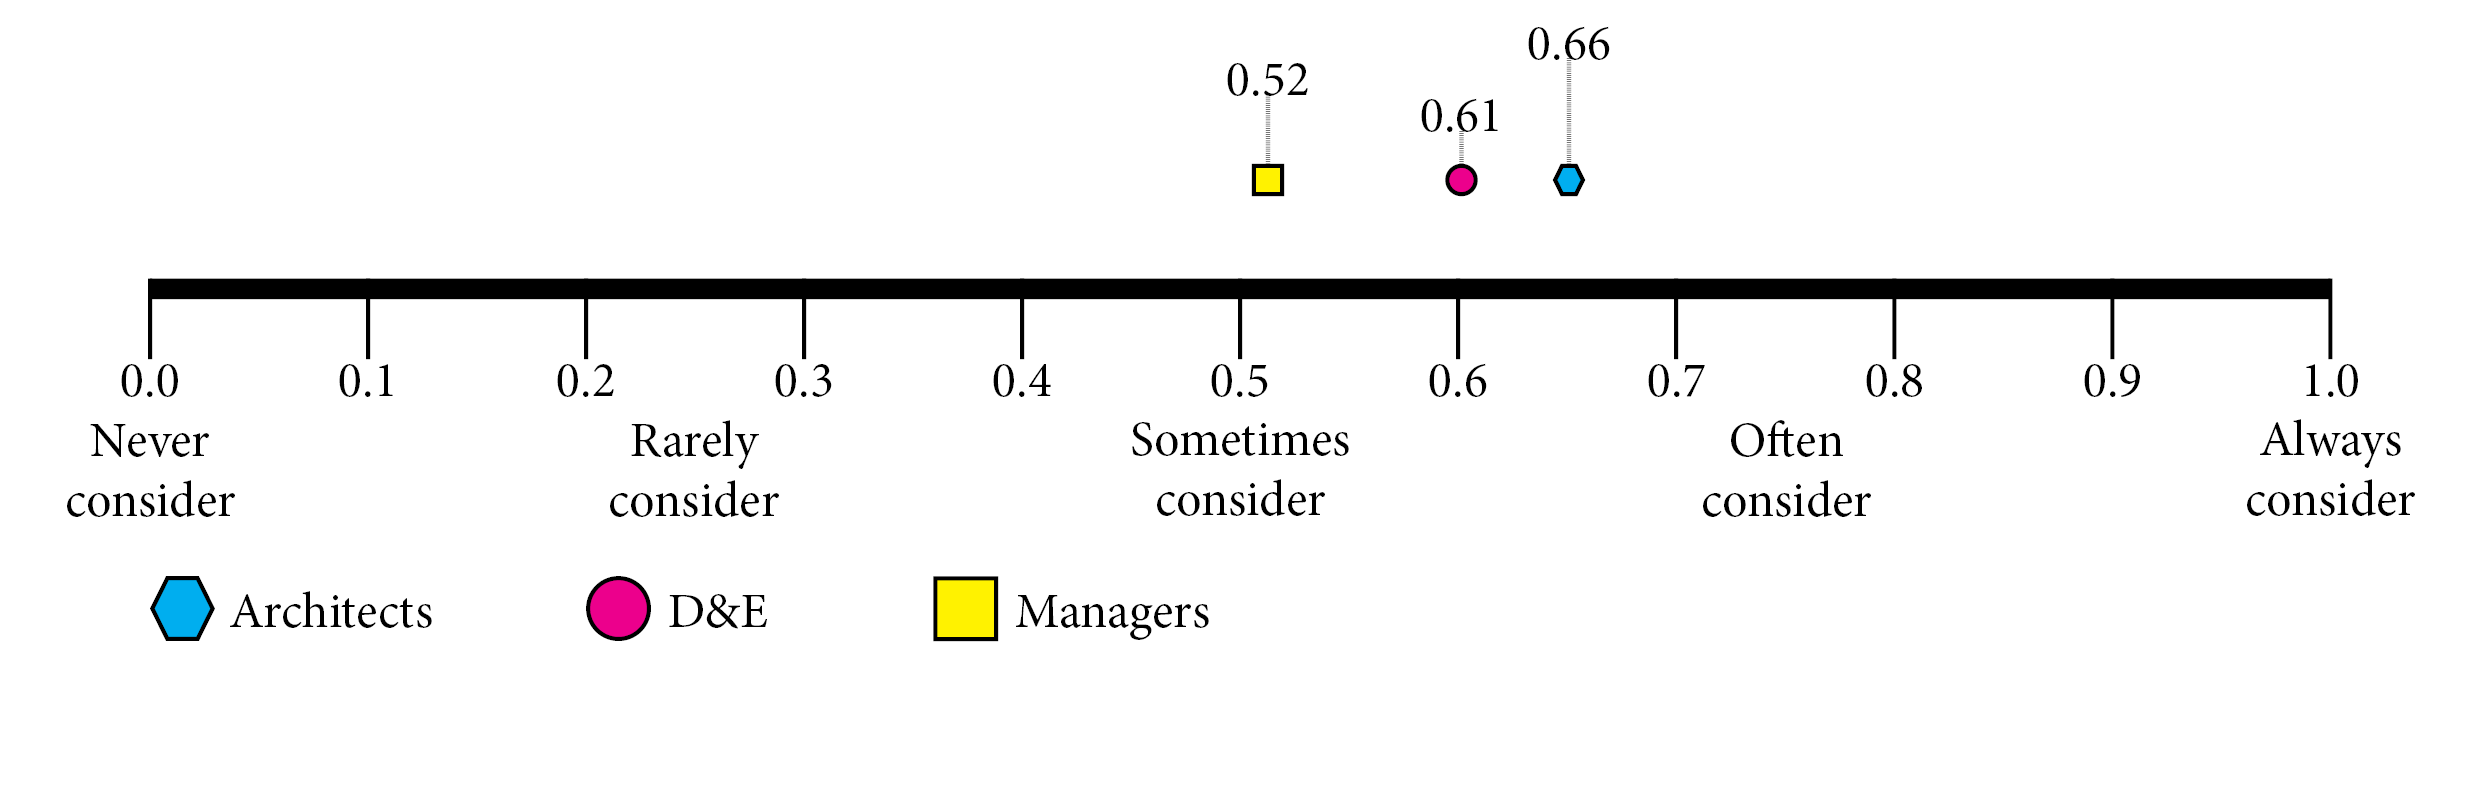
\includegraphics[width=\linewidth]{scorelines/aspect7.png}
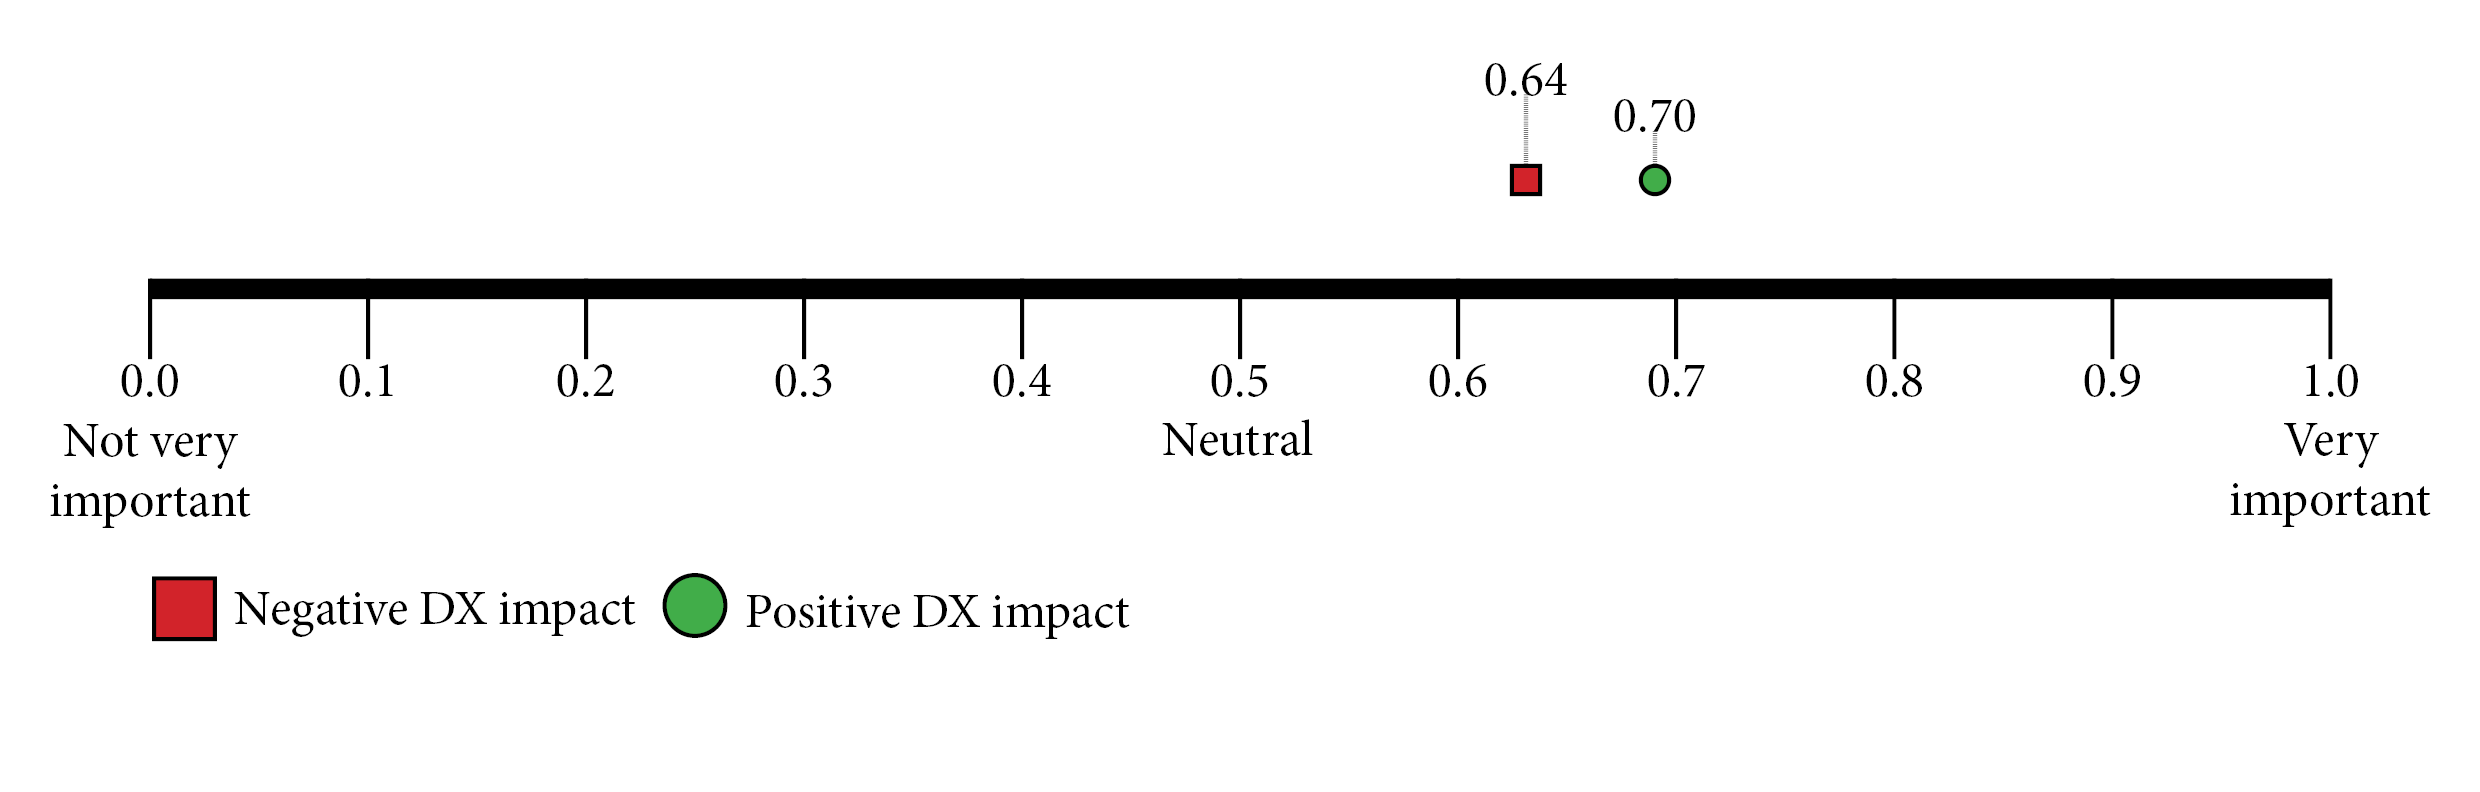
\includegraphics[width=\linewidth]{dxscorelines/dxaspect7.png}
\caption{Scoring for "The documentation is easy to navigate"}
\label{fig:aspect7}
\end{figure}
As mentioned before, developers are impatient people. A documentation that is easy to navigate, means developers can find what they're looking for quicker. In figure \ref{fig:aspect7} we see that it scored close scored somewhere in between 'Sometimes consider' and 'Often consider'. It also has a DX impact that is above neutral. The recommendation is therefor to have a clear navigation structure, with carefully chosen titles that makes the user understand what each link will lead them to. For larger pages, having a table of contents at the top that shows what sections it contains is also recommended. For smaller sub-pages a short paragraph could be good to explain to the user what he or she can expect to find on the page. This gives the possibility to the user to be more efficient when searching for specific things. The effort to do this can be somewhat high, especially the careful title naming. The titles can easily be too vague or ambivalent. Having an efficient search function for your documentation will also make the navigation more easy. To implement this is a higher effort than structuring the documentation. We therefor recommend to start with the structure, and after that work on the search function. \\ \\
\textbf{Verdict: Somewhat important, keep in mind. Medium-high effort, medium payoff.}

\subsubsection{The official website looks professional}
\begin{figure}[H]
\centering
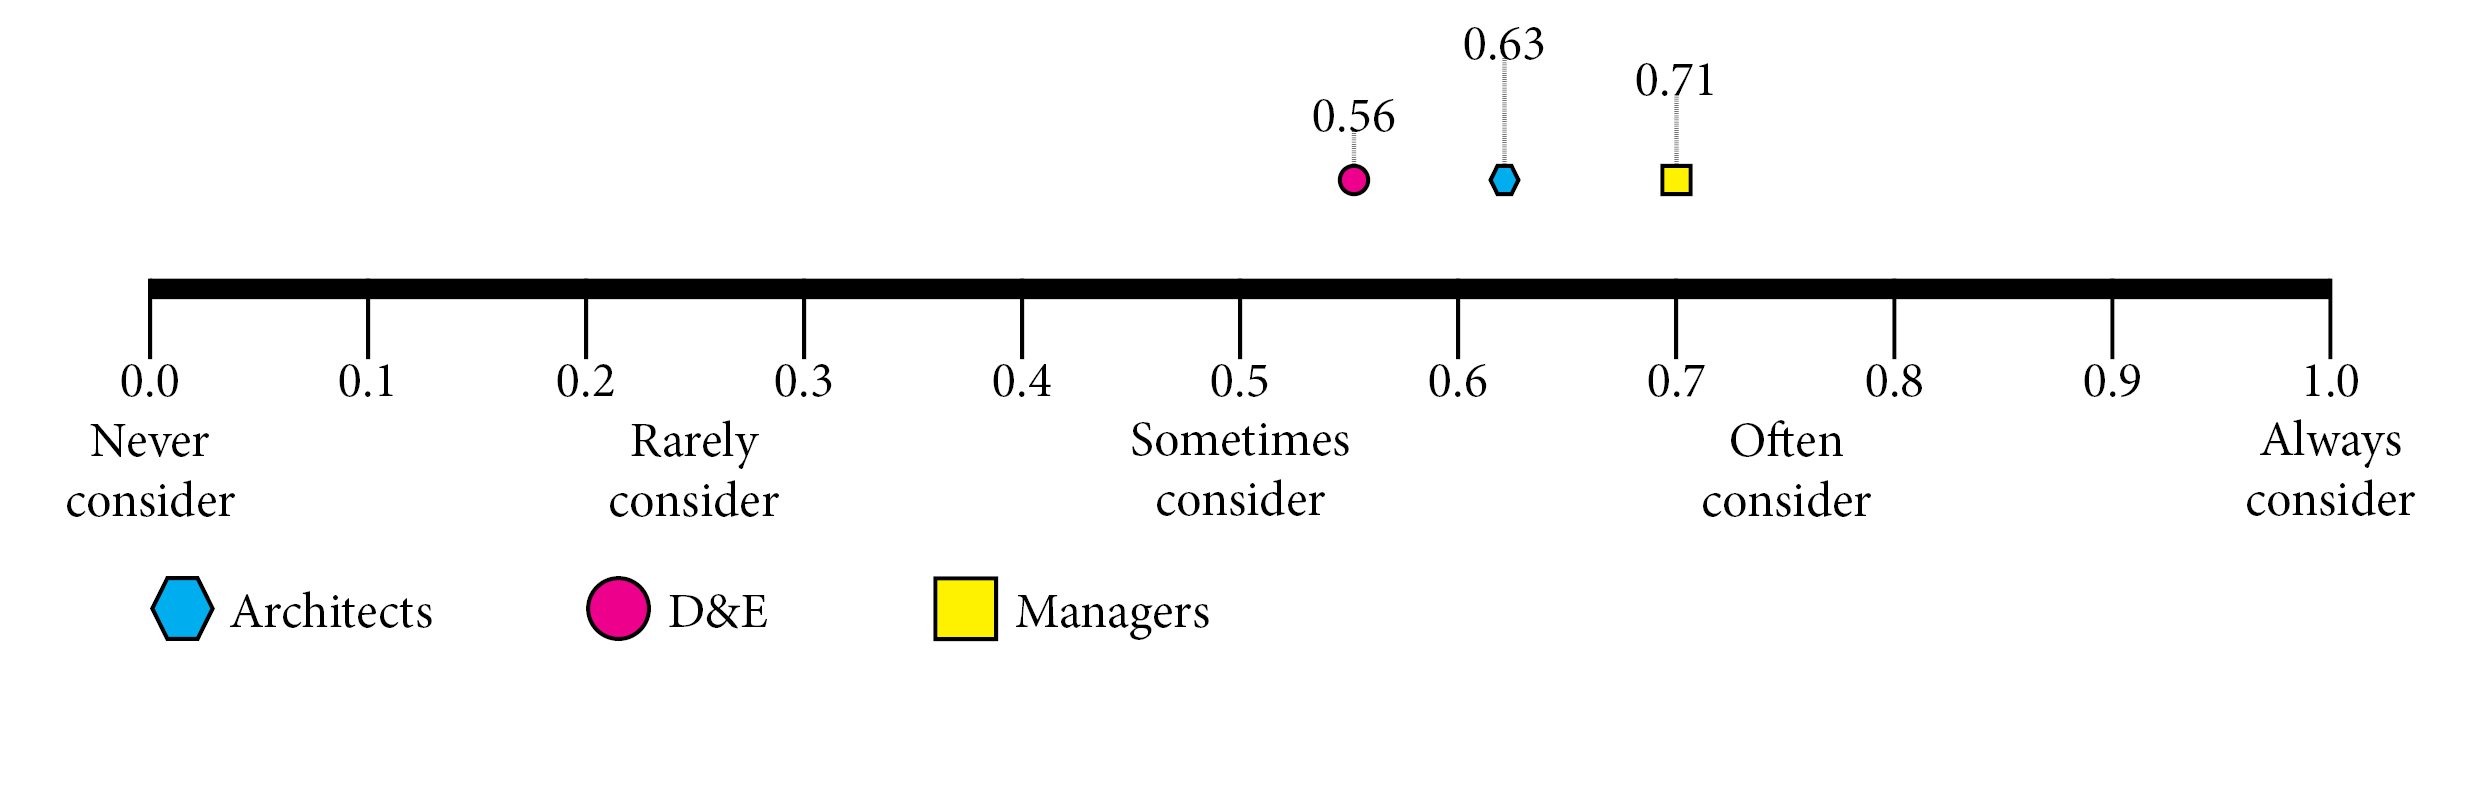
\includegraphics[width=\linewidth]{scorelines/aspect8.png}
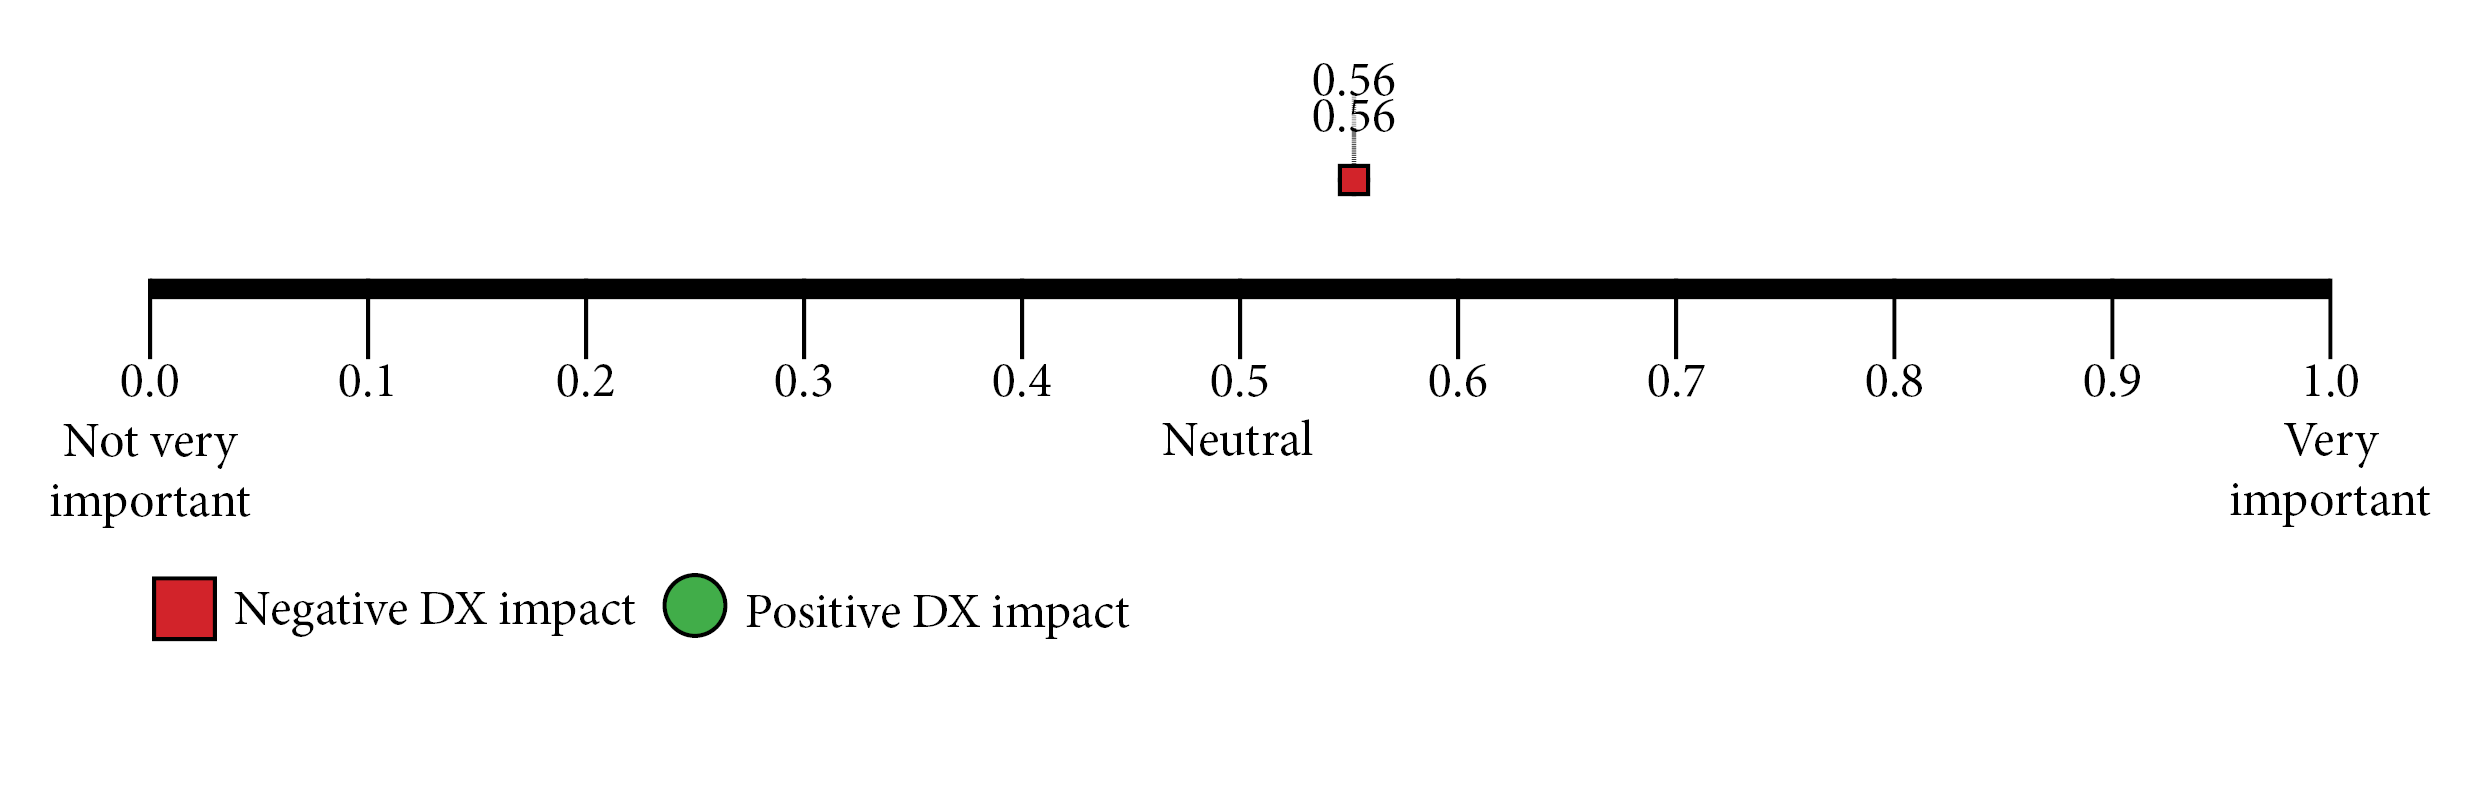
\includegraphics[width=\linewidth]{dxscorelines/dxaspect8.png}
\caption{Scoring for "The official website looks professional"}
\label{fig:aspect8}
\end{figure}
The official website is often a company's face outwards, and a user's first encounter with the company. You should not downplay the importance of first impressions. In figure \ref{fig:aspect8} we can see that it scored somewhere in between 'Sometimes consider' and 'Often consider' with the average score of 0.60/1.00. The DX-impact for a good or bad website is however neutral. The recommendation is to spend some time to make sure your official website looks professional. Test it for different browsers and devices. The effort to do this should not be high for a software company who creates software platforms. If a company whom provides software platform solutions cannot provide a professional looking website, the impression it gives is that they won't provide a good platform either. As seen in figure \ref{fig:aspect8} it's more important to managers. If you cater to these, this aspect is even more important.
\\ \\
\textbf{Verdict: Somewhat important, keep in mind. Medium effort, medium payoff.}

\subsubsection{The pricing of the software}
\begin{figure}[H]
\centering
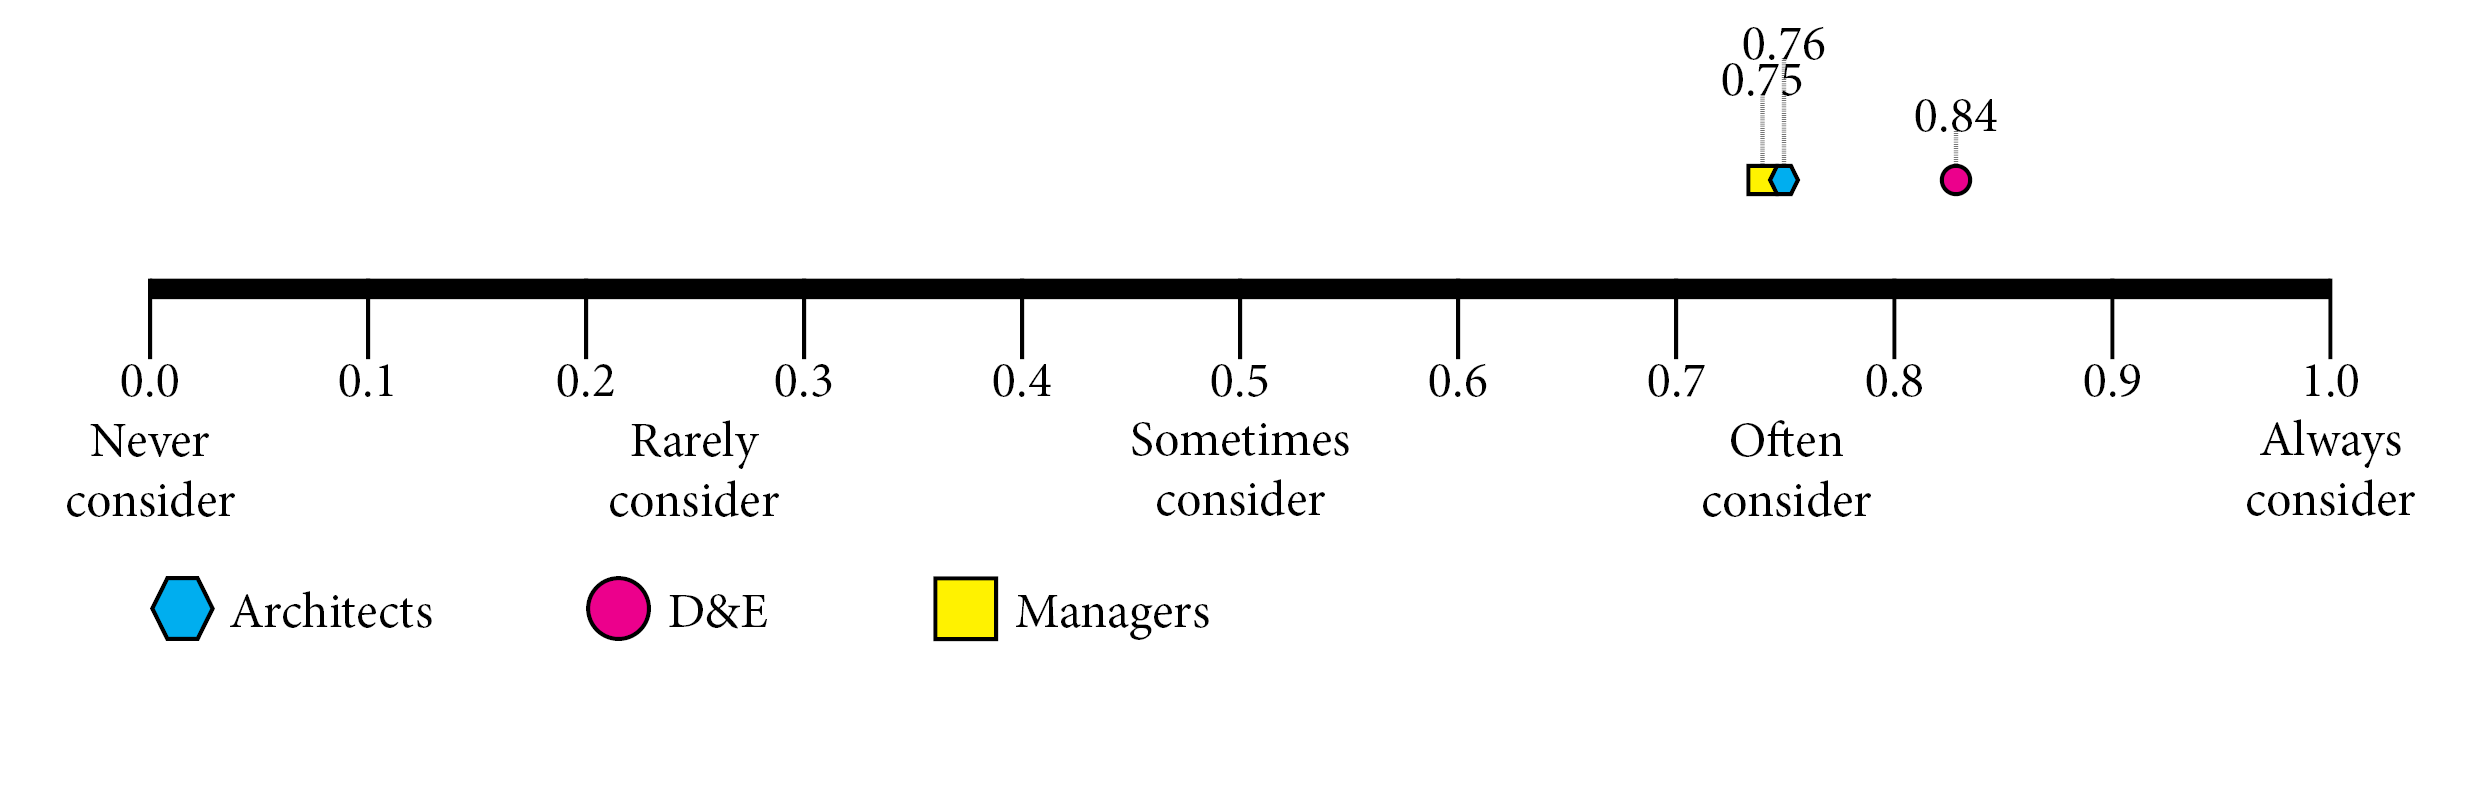
\includegraphics[width=\linewidth]{scorelines/aspect9.png}
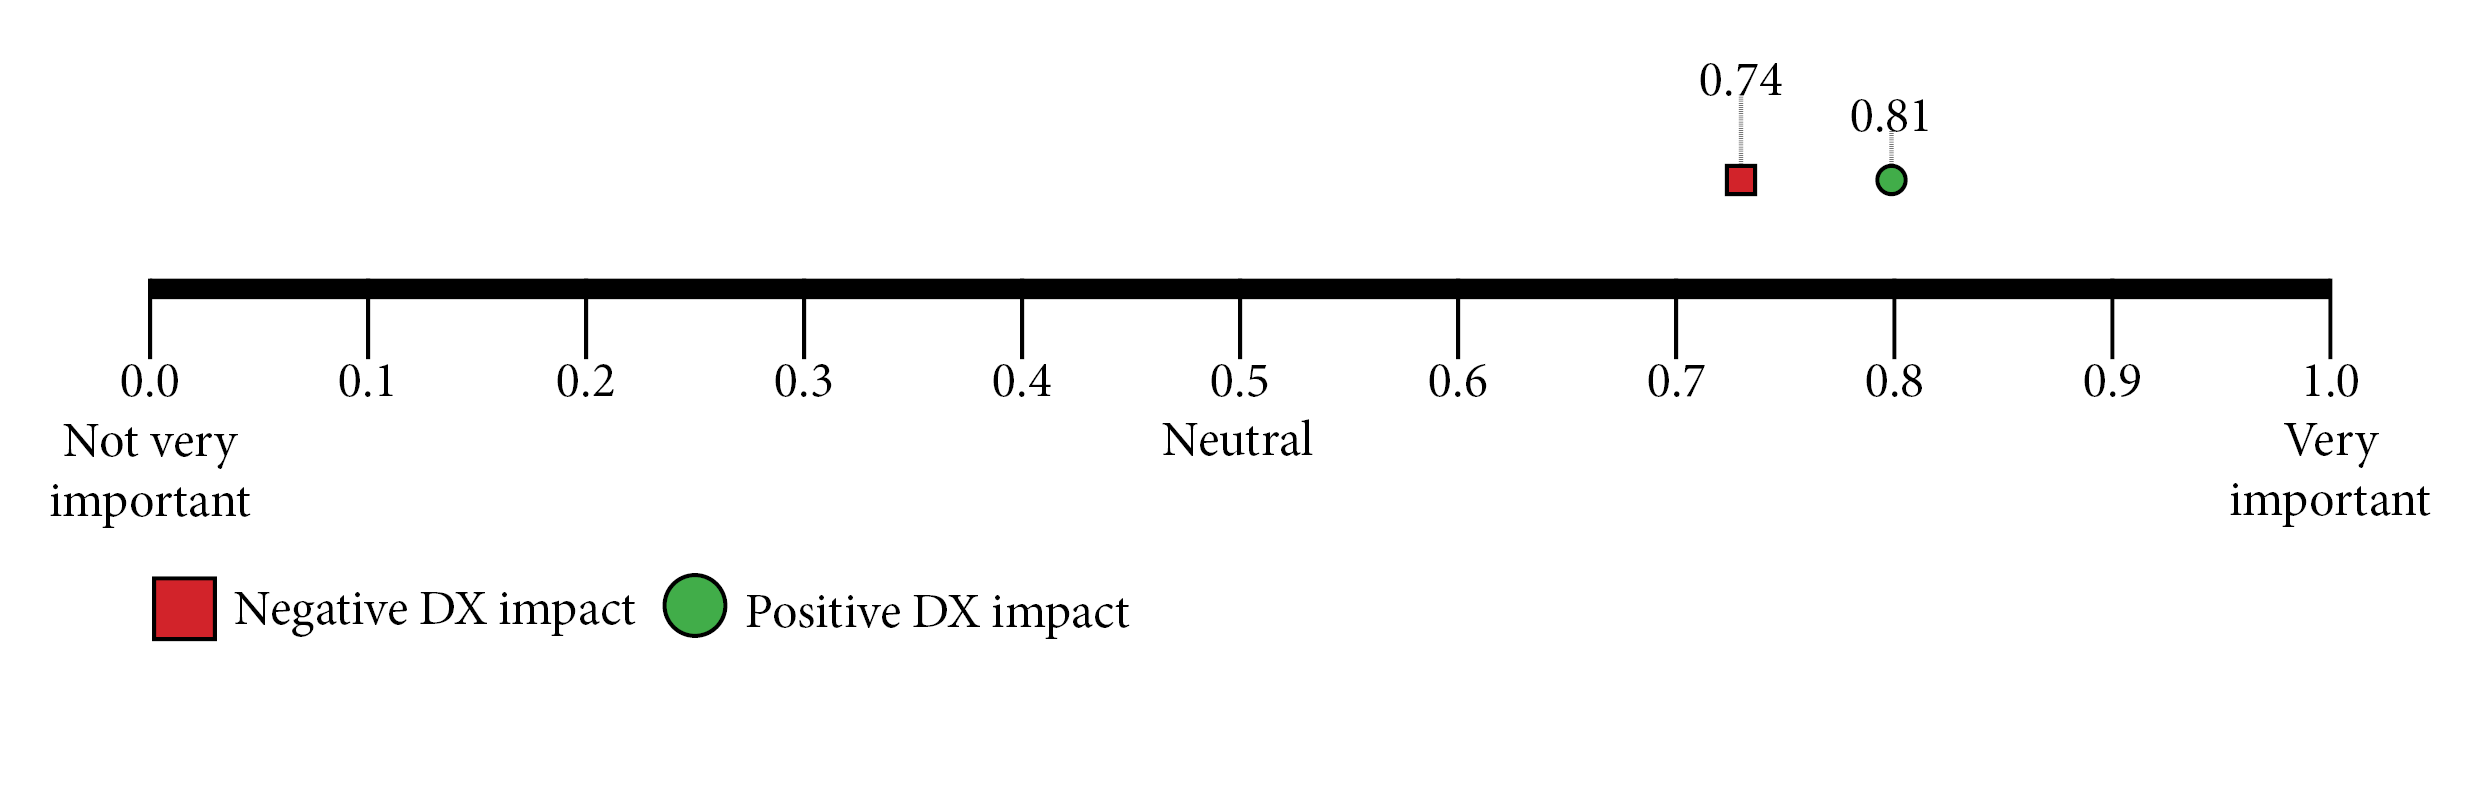
\includegraphics[width=\linewidth]{dxscorelines/dxaspect9.png}
\caption{Scoring for "The pricing of the software"}
\label{fig:aspect9}
\end{figure}
Money always plays a roll in any company, and the price of a software cannot be ignored. You can make money from your software in many ways, through licensing, subscriptions, support contract, and more. It's out of the scope of this research paper on how one should make money from software platforms. In figure \ref{fig:aspect9} we see that it's quite important to people. This is another aspect, as mentioned in section \ref{consisQuestions}, where the DX-questions and considerations questions are a bit different, and one should be careful to draw parallels. We can see however in the consideration scoring that pricing is very important. We can tell by the DX-scoring that clearly showing the pricing of the software has a very strong positive impact, and hiding the pricing away has a strong negative impact. The recommendation for pricing, in order to give a good experience for developers, is to clearly state the pricing of the software platform. Whichever money making model the software platform uses, the cost to inquire it for a developer should not be hidden away. \\ \\
\textbf{Verdict: Important, keep in mind. Low effort, high payoff.}

\subsubsection{The release- and change notes are thorough}
\begin{figure}[H]
\centering
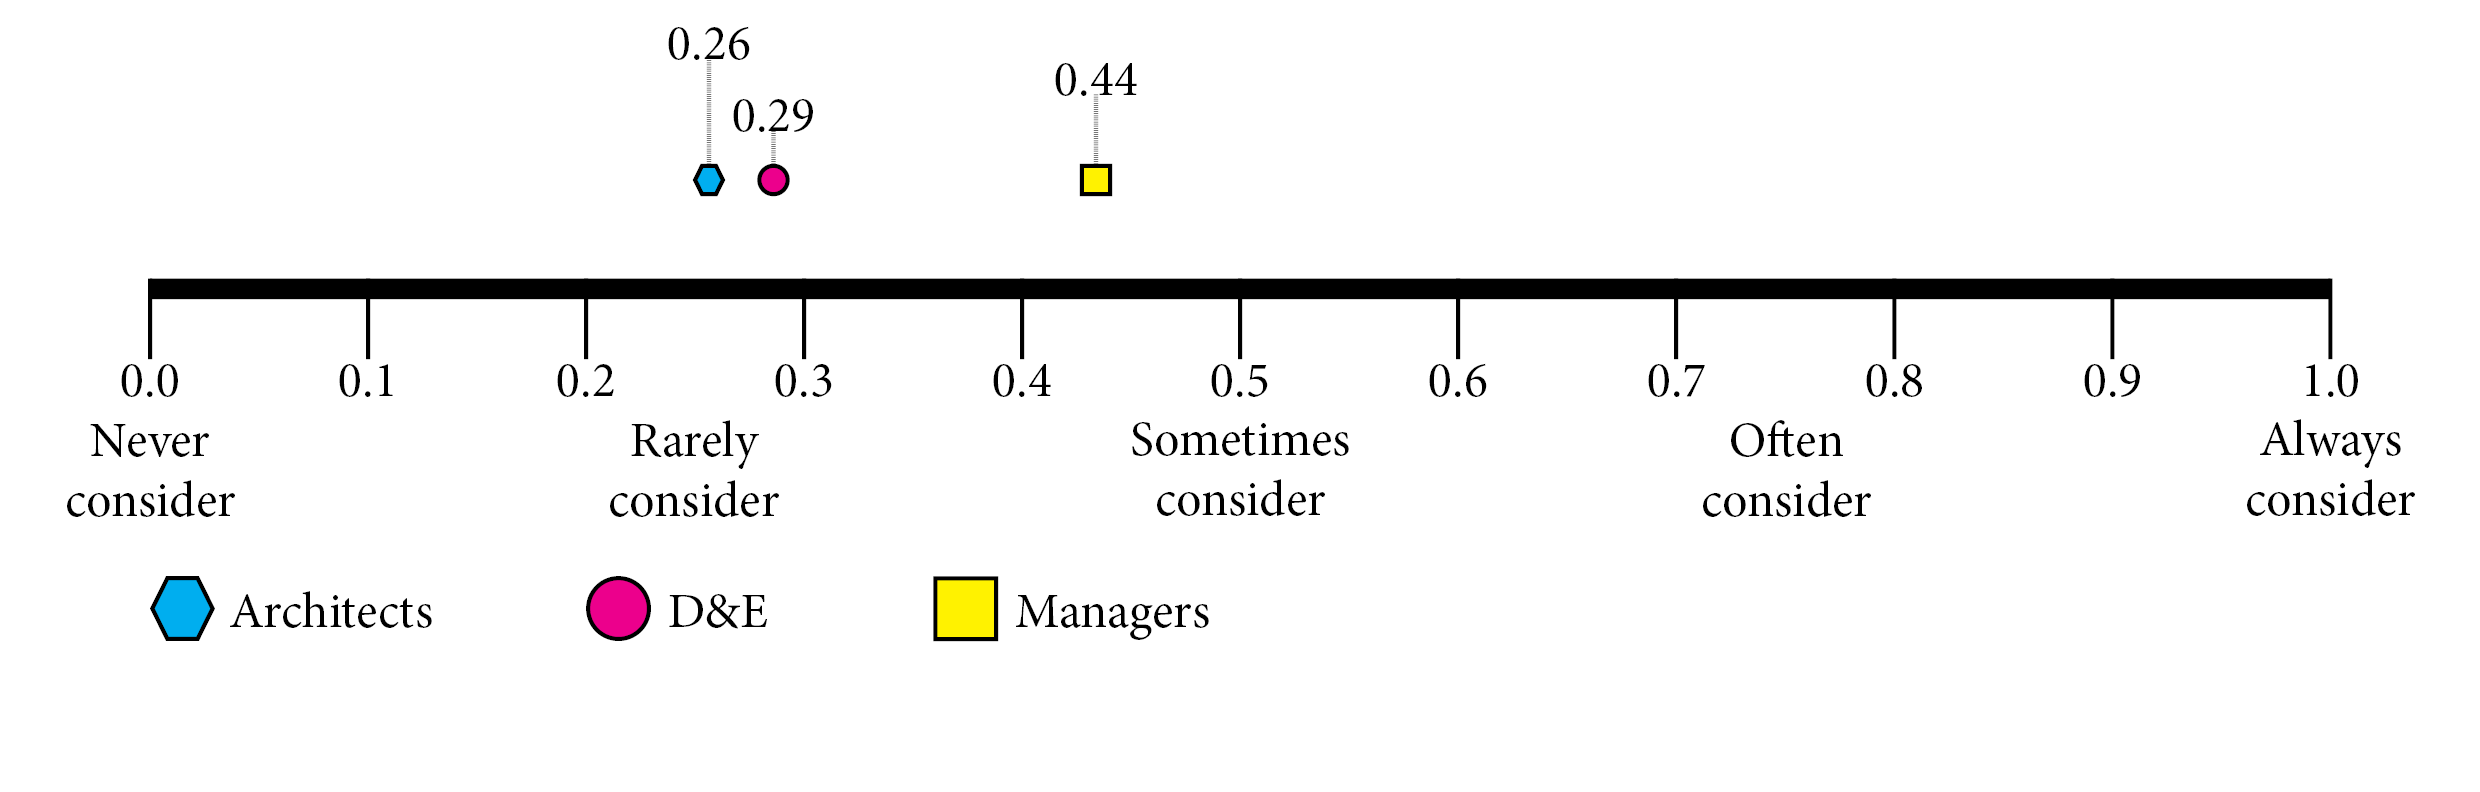
\includegraphics[width=\linewidth]{scorelines/aspect10.png}
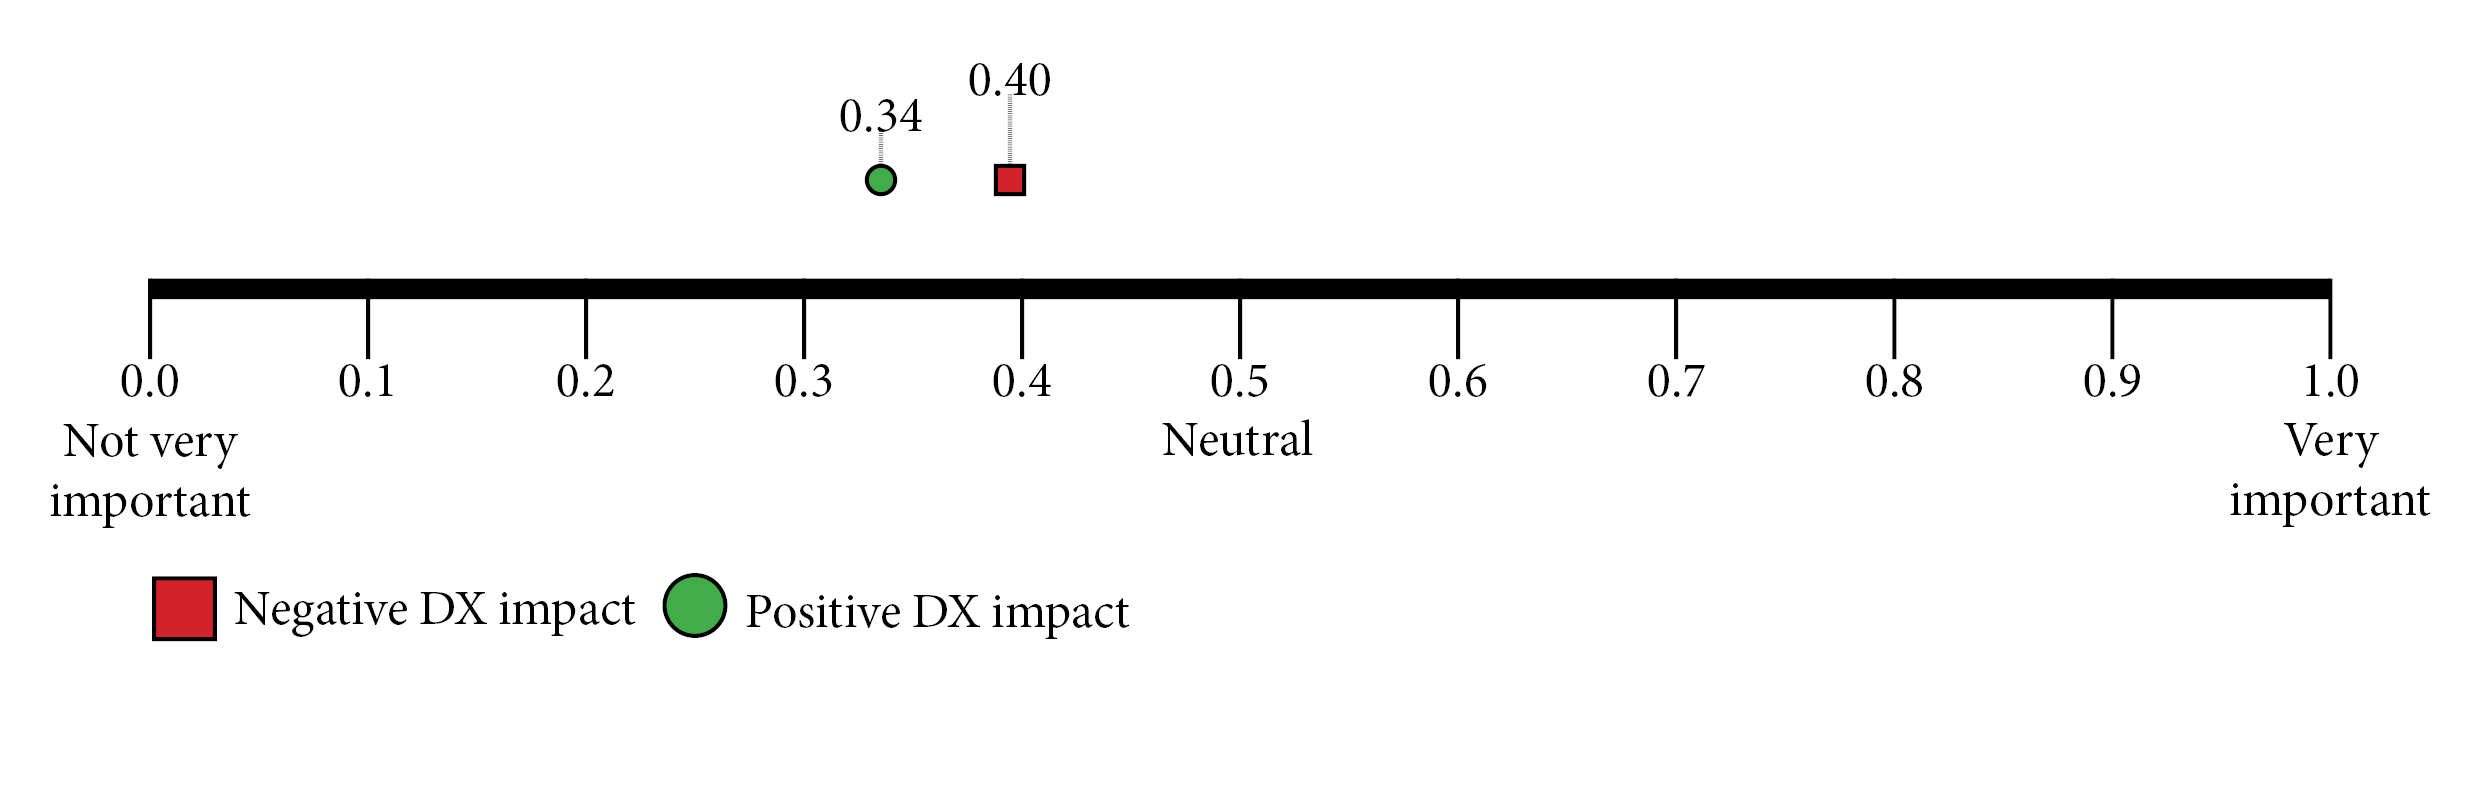
\includegraphics[width=\linewidth]{dxscorelines/dxaspect10.png}
\caption{Scoring for "The release- and change notes are thorough"}
\label{fig:aspect10}
\end{figure}
Release notes was shown to be a quite non-important aspect, as seen in figure \ref{fig:aspect10}, especially for the people who are supposedly using them: developers and architects. We can see by the DX-impact that poor release notes has a bit of a negative impact. It's however still below neutral. The interviews showed that release notes are a last resort for people, and ignored as much as possible. There recommendation is therefor to not spend too much time on release notes. But make sure to not ignore them. If you make sure to have good commit messages, these can act as a good base for writing the release notes. This minimises the time that has to be spent on writing the release notes.\\ \\
\textbf{Verdict: Not important, but don't ignore. Medium effort, low payoff.}

\subsubsection{The software has the same features on all different platforms}
\begin{figure}[H]
\centering
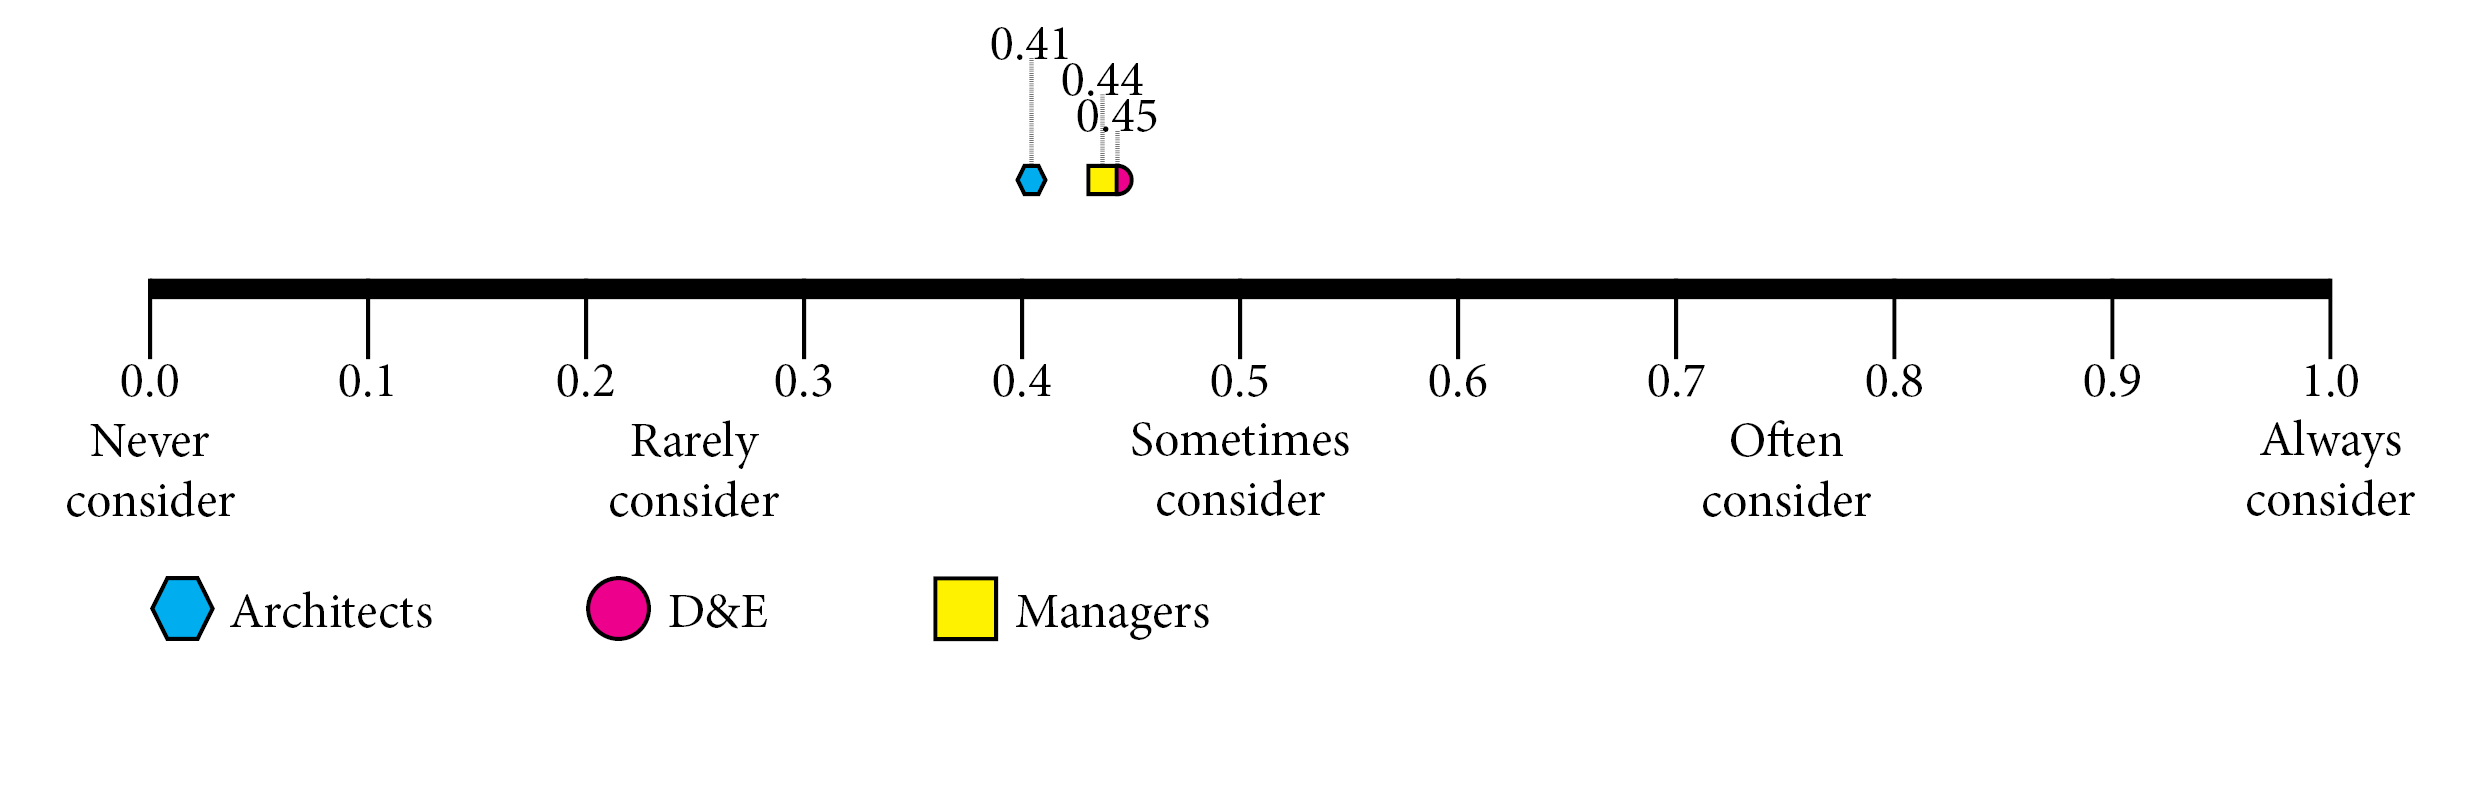
\includegraphics[width=\linewidth]{scorelines/aspect11.png}
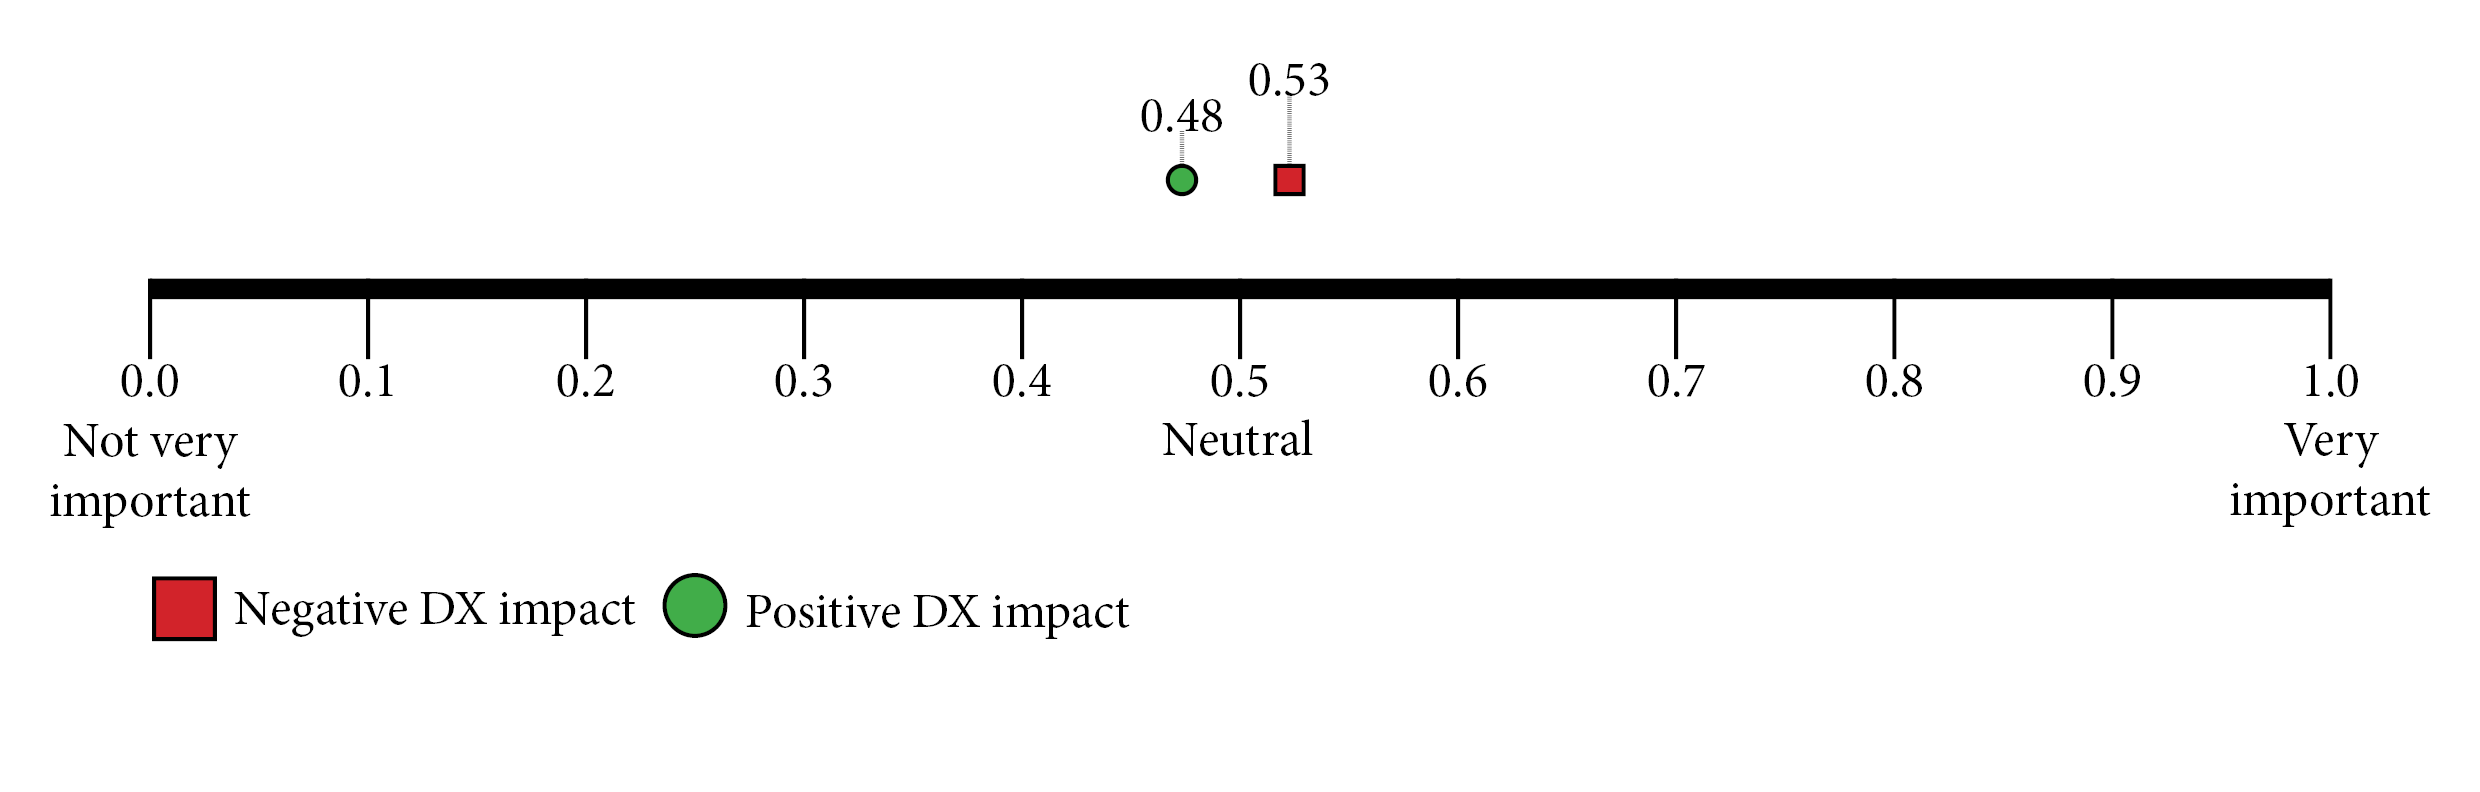
\includegraphics[width=\linewidth]{dxscorelines/dxaspect11.png}
\caption{Scoring for "The software has the same features on all different platforms"}
\label{fig:aspect11}
\end{figure}
If your software platform supports many different platforms, such as operation systems and browsers, it's takes time and effort to make sure that they work the same in all situations. In figure \ref{fig:aspect11} we see that this scores kind of low, and the DX-impact is neutral. The effort to make sure that all features exist on all platforms is very high. The recommendation is therefor to clearly state to the users what features are offered on what platforms. But be aware that the effort to keep the features consistent on all platforms may not have a big payoff. \\ \\
\textbf{Verdict: Not very important. High effort, low-medium payoff.}

\subsubsection{The software is compatible with different platforms}
\begin{figure}[H]
\centering
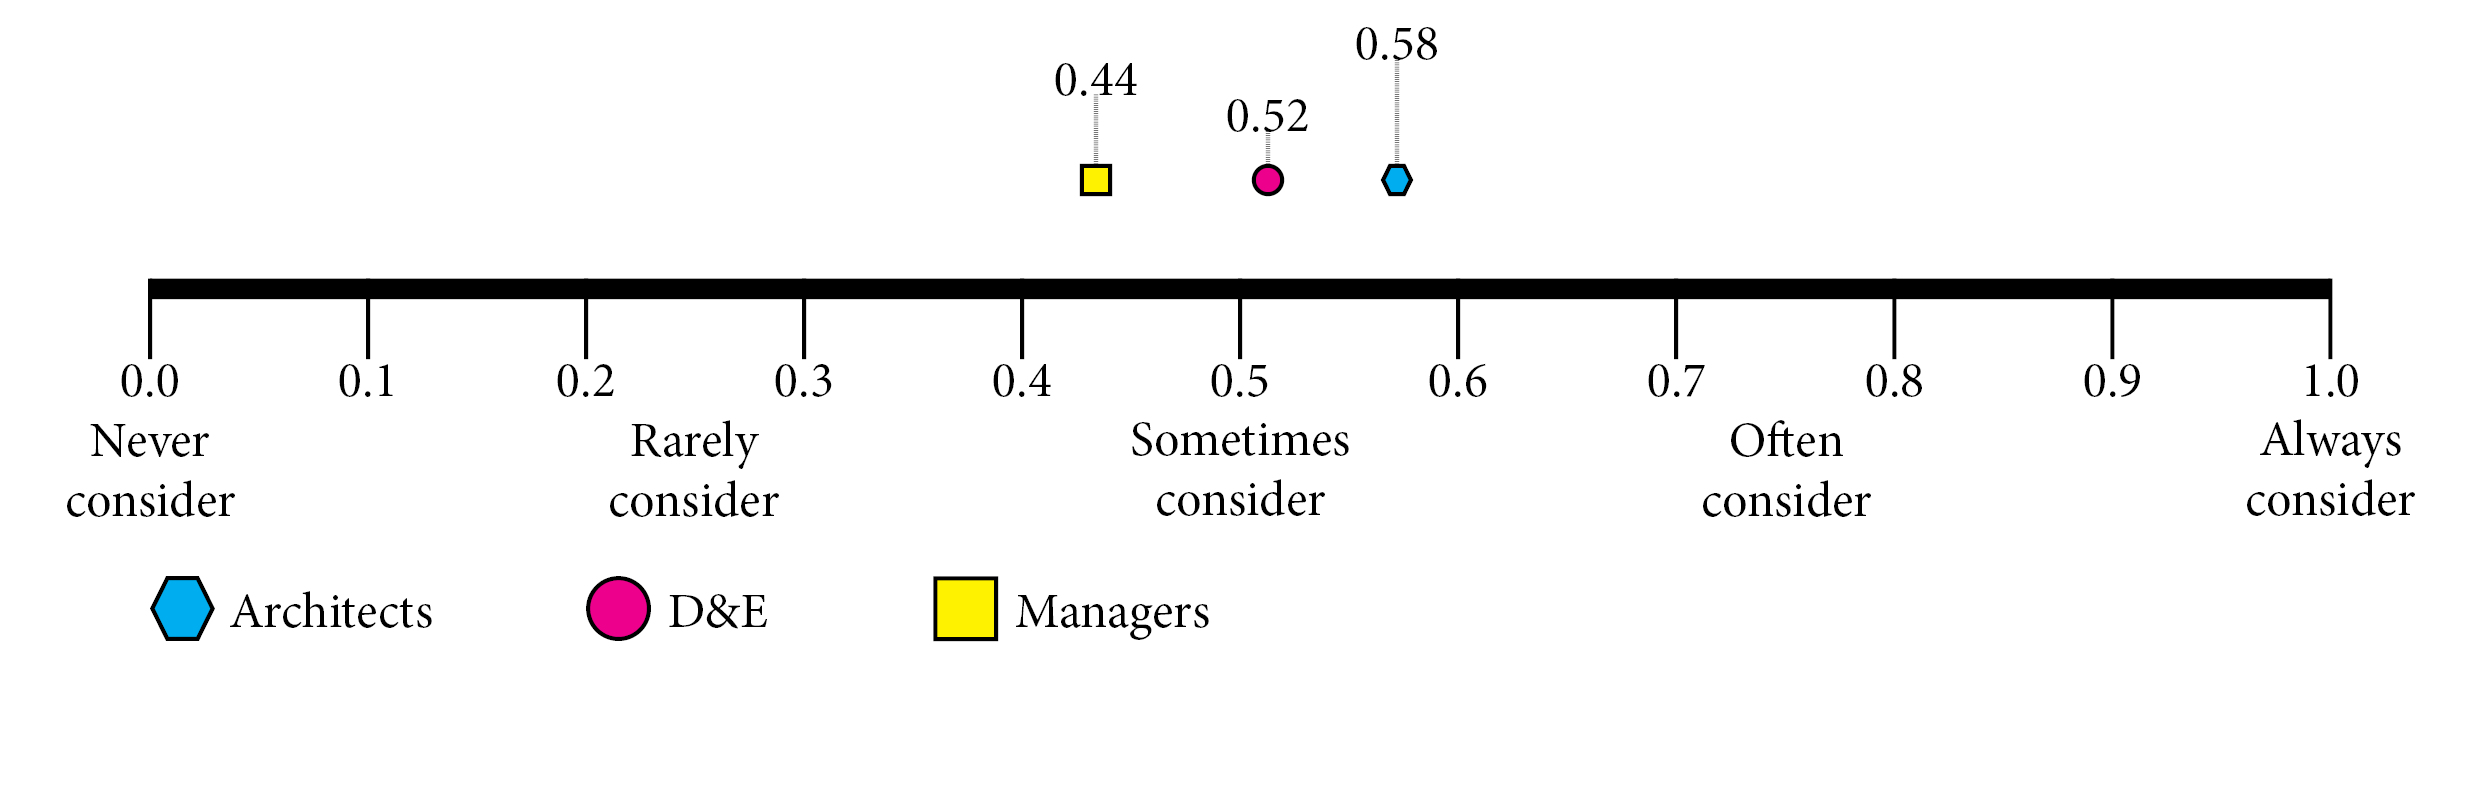
\includegraphics[width=\linewidth]{scorelines/aspect12.png}
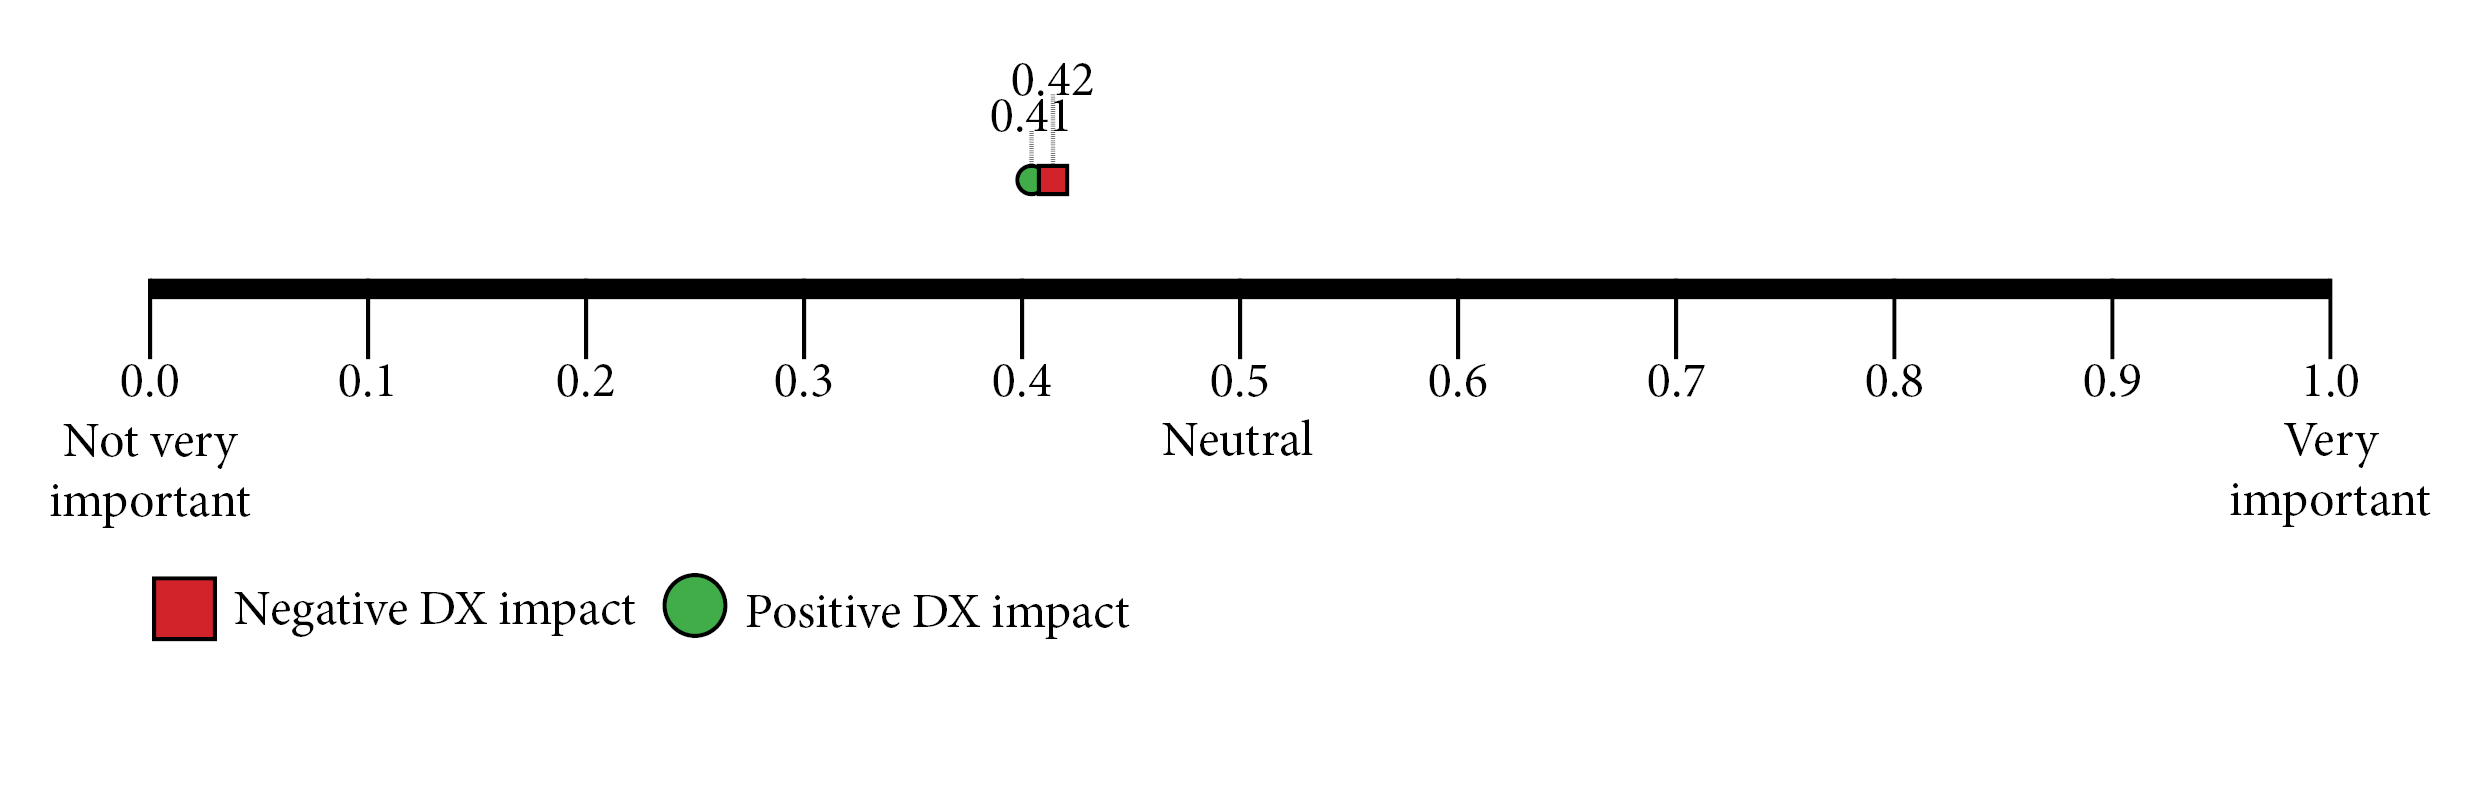
\includegraphics[width=\linewidth]{dxscorelines/dxaspect12.png}
\caption{Scoring for "The software is compatible with different platforms"}
\label{fig:aspect12}
\end{figure}
Having your software platform be compatible with many different platforms is a requirement for some users, a bonus for some. The effort to do this is however high. If you plan to implement this, make sure that the increase in potential users is worth the effort to do this. You need to be aware that is highly increases all future maintenance for your platform. As we can see in figure \ref{fig:aspect12}, it does not score very high, and the DX impact is even less. The recommendation is therefor to skip this aspect, if you are not sure that the increase in users is worth the effort. \\ \\
\textbf{Verdict: Not very important. High effort, low-medium payoff.}

\subsubsection{The software is offered in more than one programming language}
\begin{figure}[H]
\centering
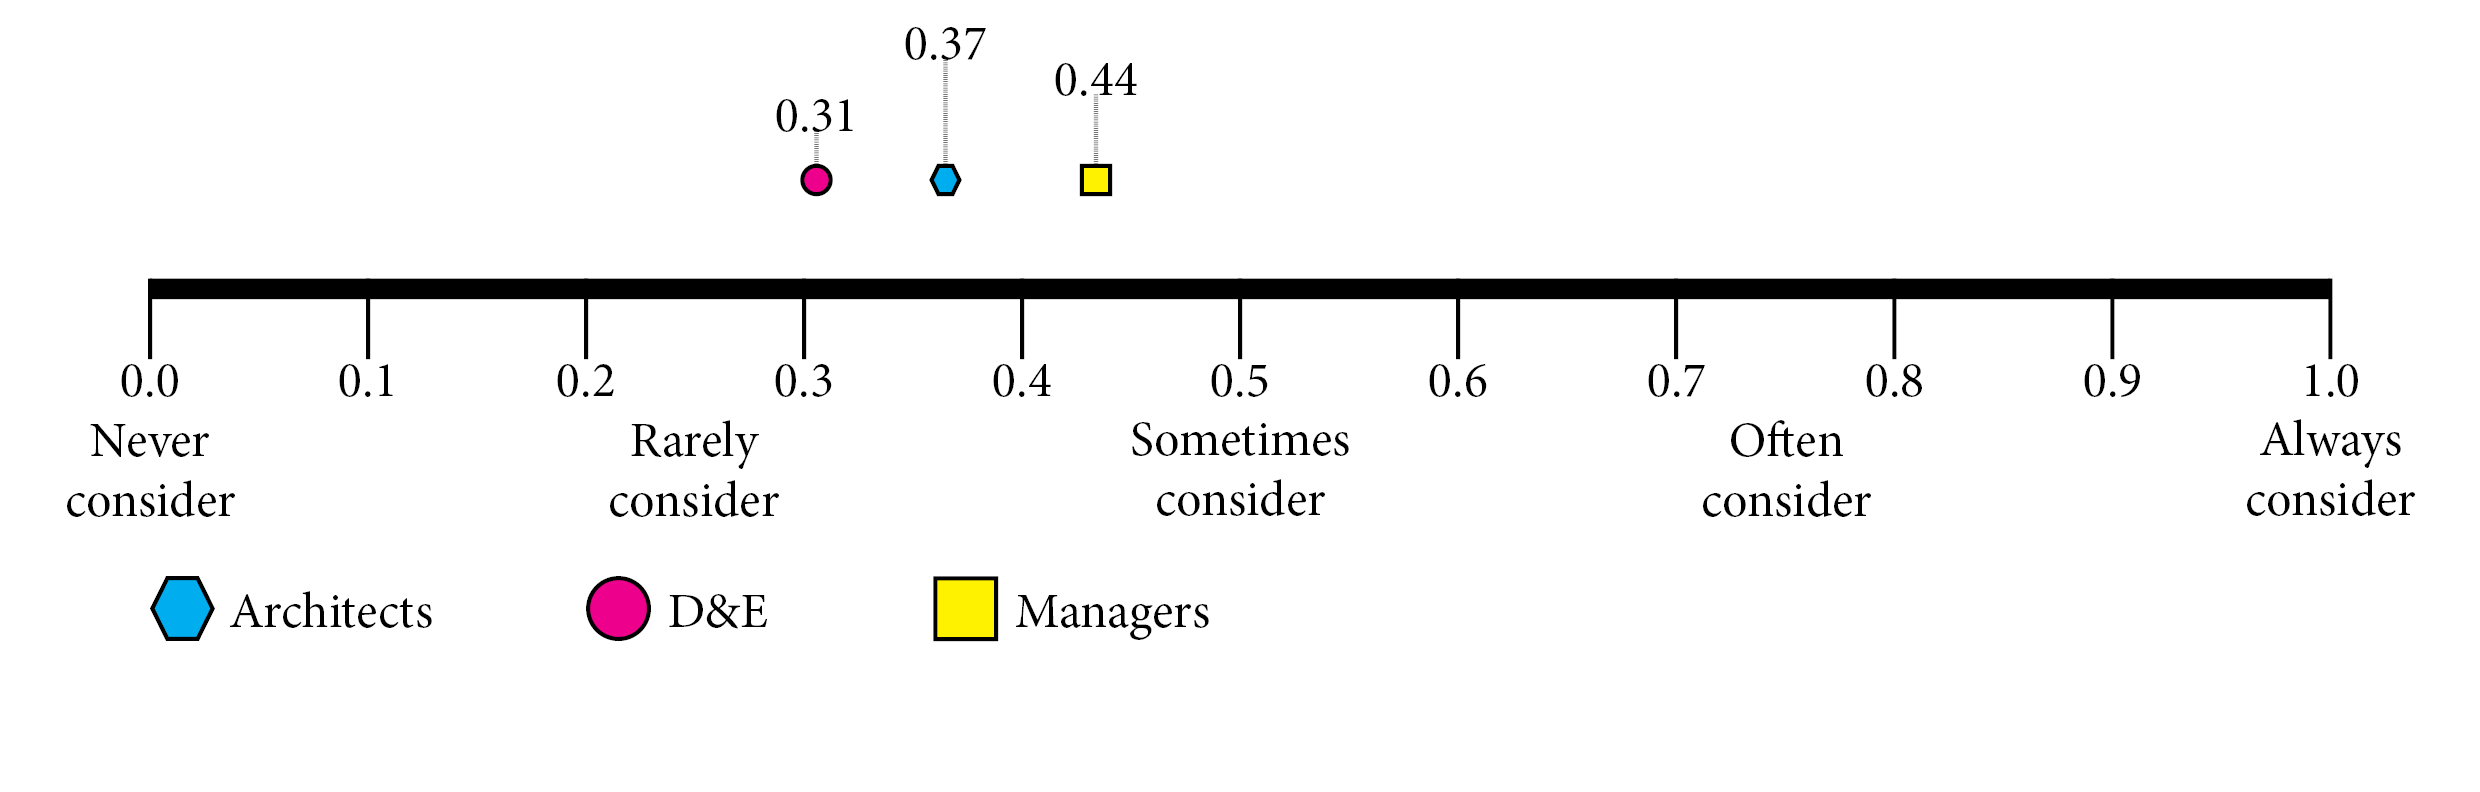
\includegraphics[width=\linewidth]{scorelines/aspect13.png}
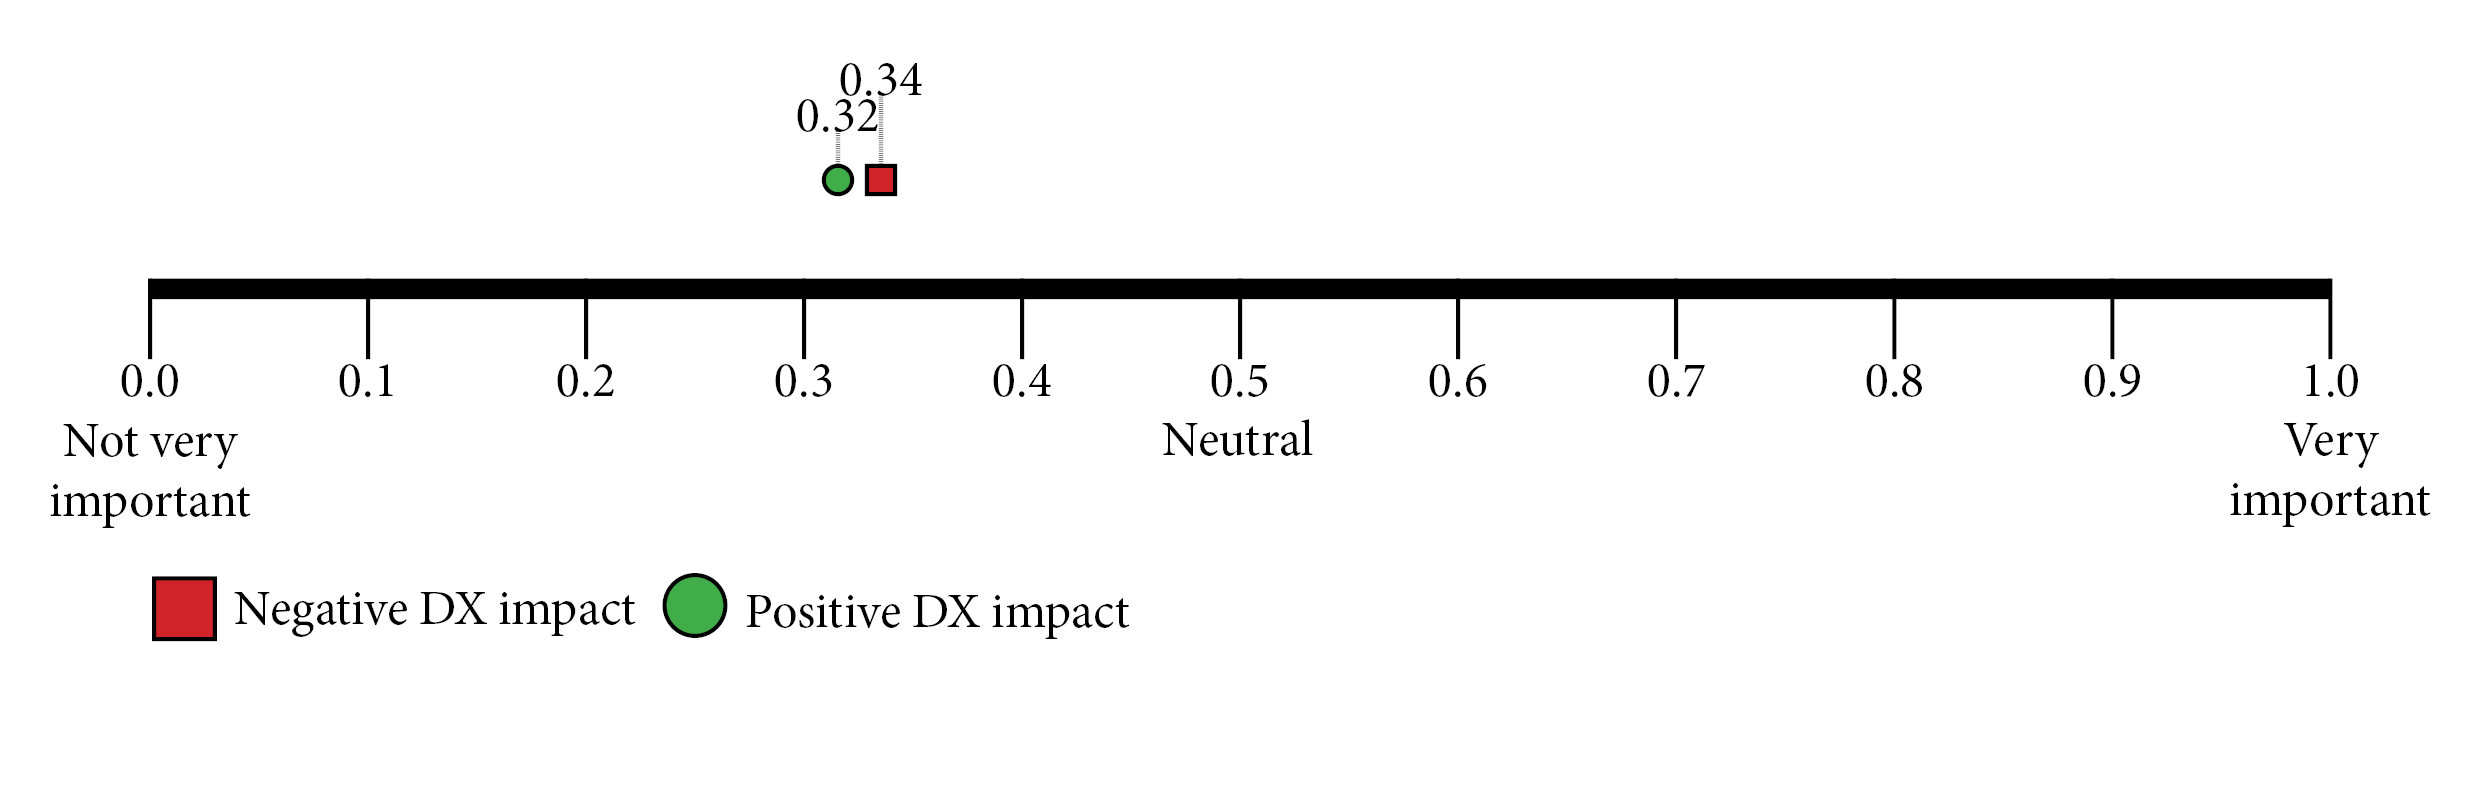
\includegraphics[width=\linewidth]{dxscorelines/dxaspect13.png}
\caption{Scoring for "The software is offered in more than one programming language"}
\label{fig:aspect13}
\end{figure}
Having your platform be compatible with more than one language takes a big effort. It takes a long time to develop and doubles the maintenance needed. As we can see in figure \ref{fig:aspect13} it's not ranked high at all, both for the consideration part and the DX part. The recommendation is therefor to ignore this aspect. The effort compared with the payoff is not worth it. \\ \\
\textbf{Verdict: Not important. High effort, low payoff.}

\subsubsection{The software is open source}
\begin{figure}[H]
\centering
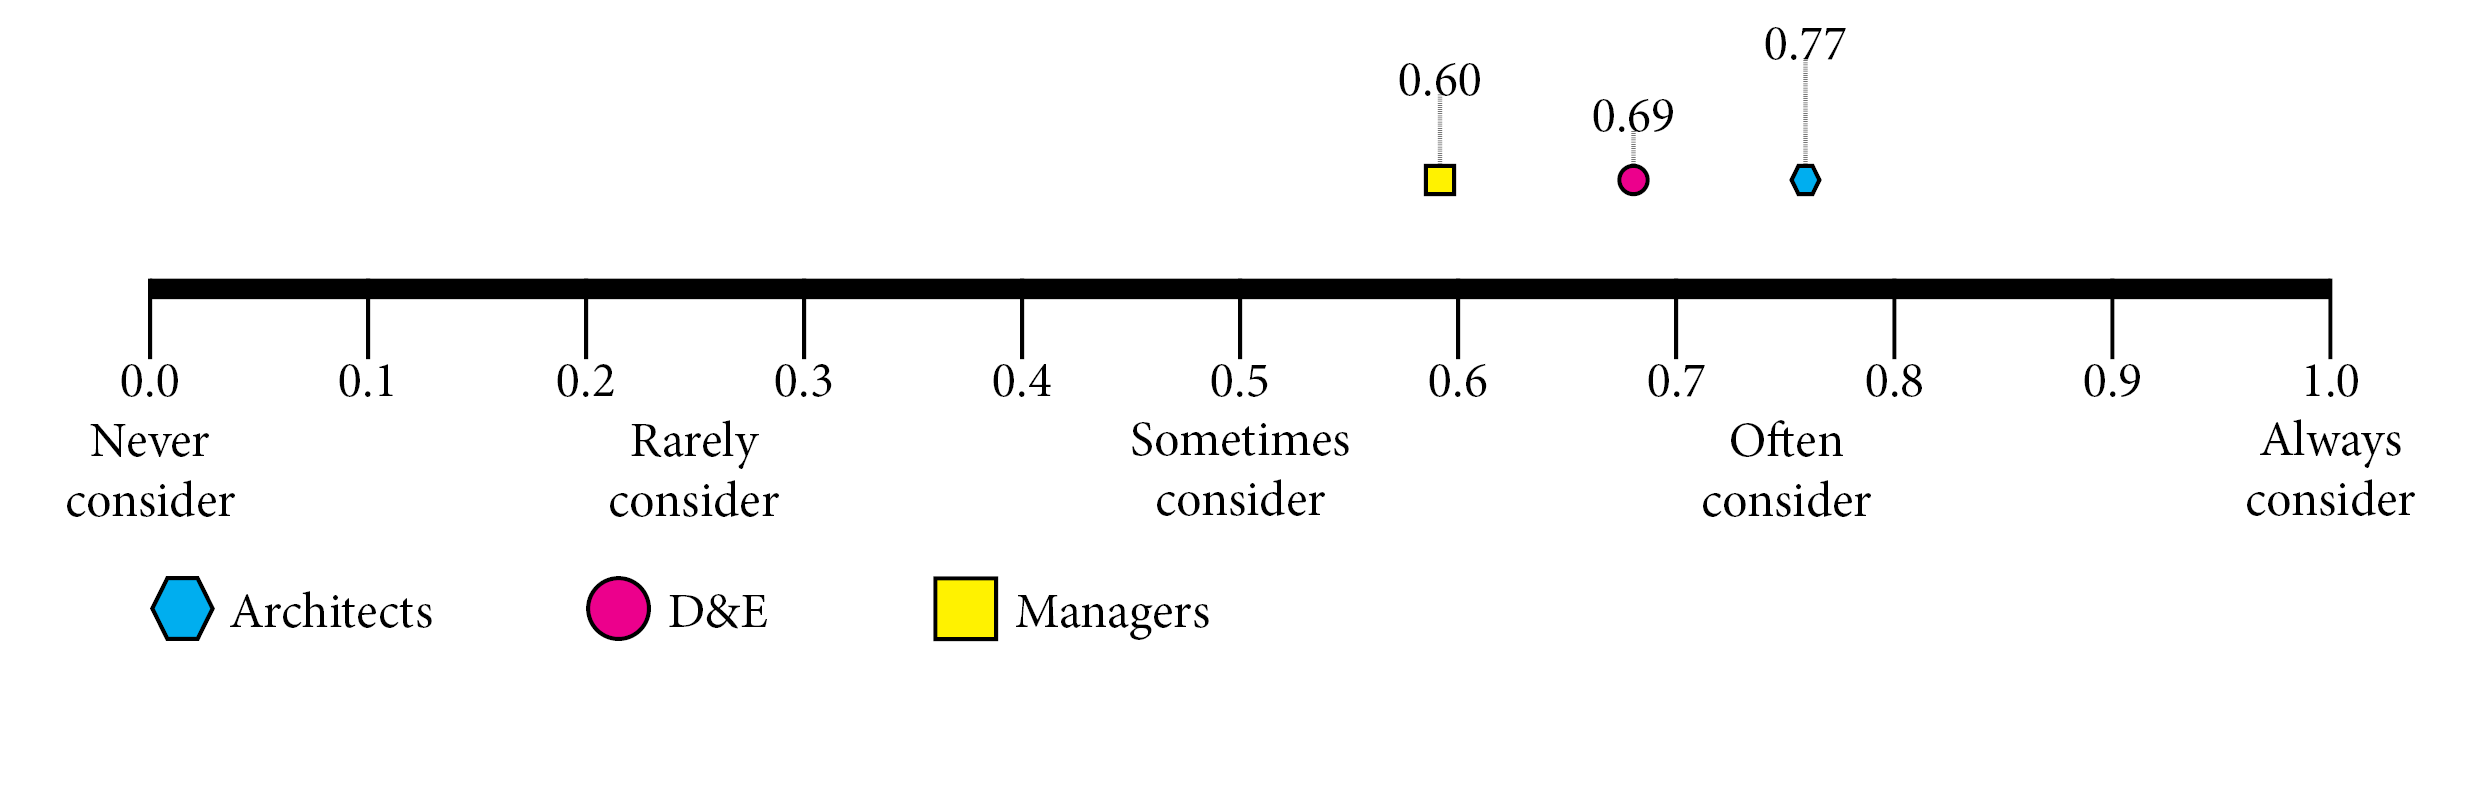
\includegraphics[width=\linewidth]{scorelines/aspect14.png}
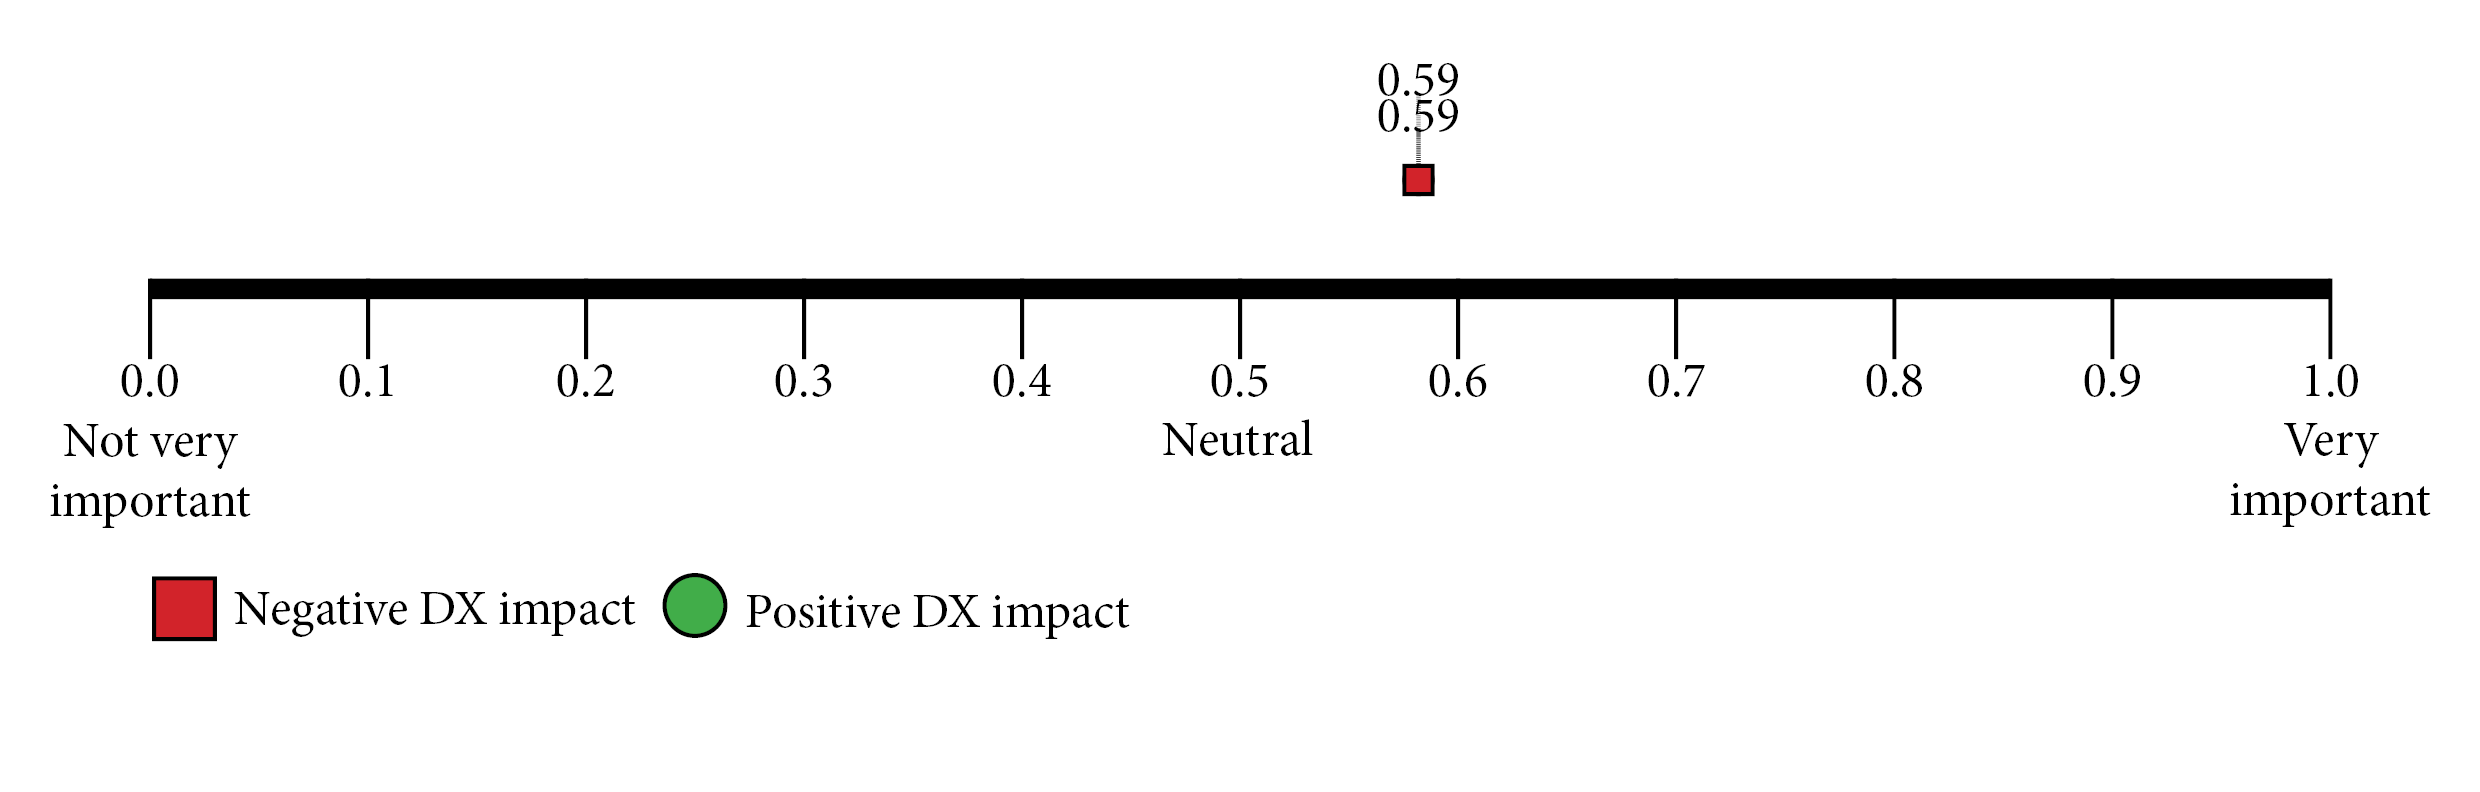
\includegraphics[width=\linewidth]{dxscorelines/dxaspect14.png}
\caption{Scoring for "The software is open source"}
\label{fig:aspect14}
\end{figure}
Being open source has both benefits and limitations. It is out of the scope of this research paper to evaluate these. But as we can see in figure \ref{fig:aspect14} it's quite important to developers and architects. The DX impact shows however that being close-sourced doesn't have a very big impact. The recommendation is therefor to try to be open source if you can, but it's not necessary. If it's not something that the company is used to, be aware that it requires other ways of working than conventional software that is close-source. If you decide to make an open-source software platform, make you have the expertise in the company to be able to handle this type of software. It has a potential to increase the amount of users, but if you don't use the benefits that open-source gives, it may not pay off. \\ \\
\textbf{Verdict: Important. Medium-high effort, high payoff.}

\subsubsection{The software uses the programming language I am most comfortable with}
\begin{figure}[H]
\centering
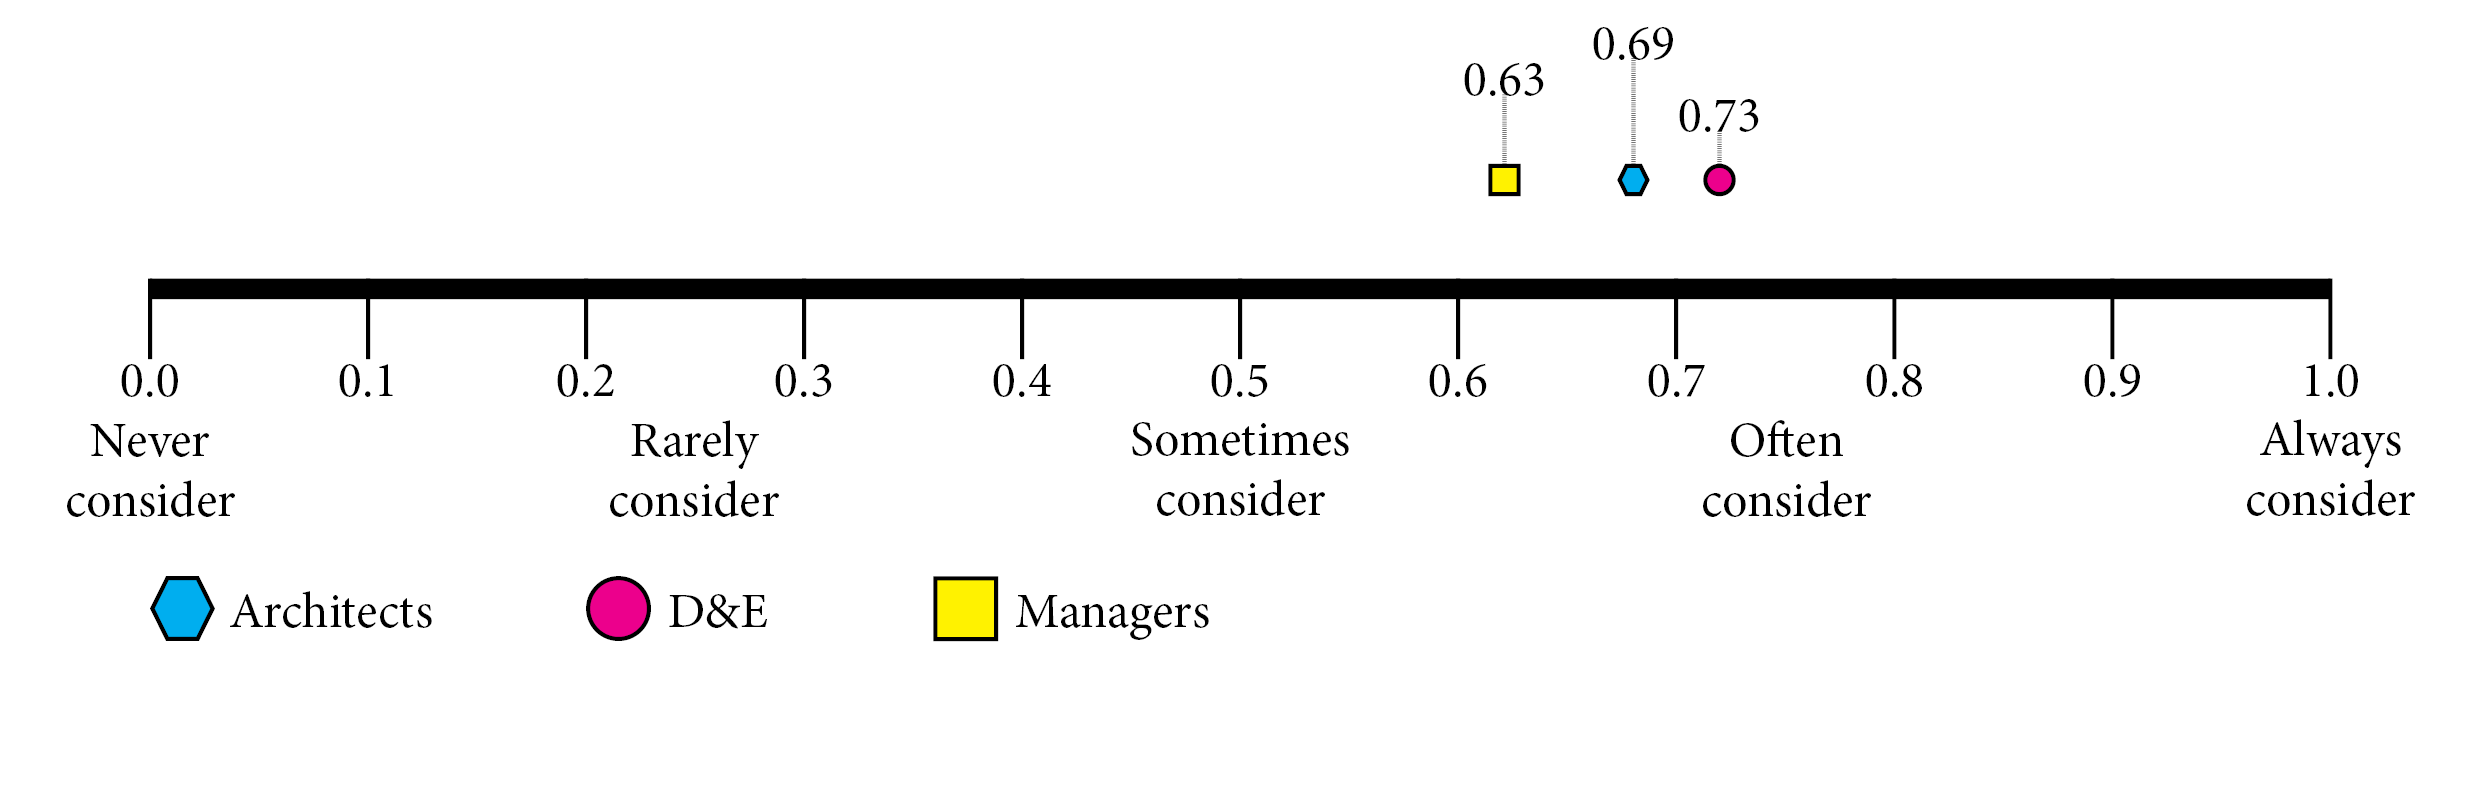
\includegraphics[width=\linewidth]{scorelines/aspect15.png}
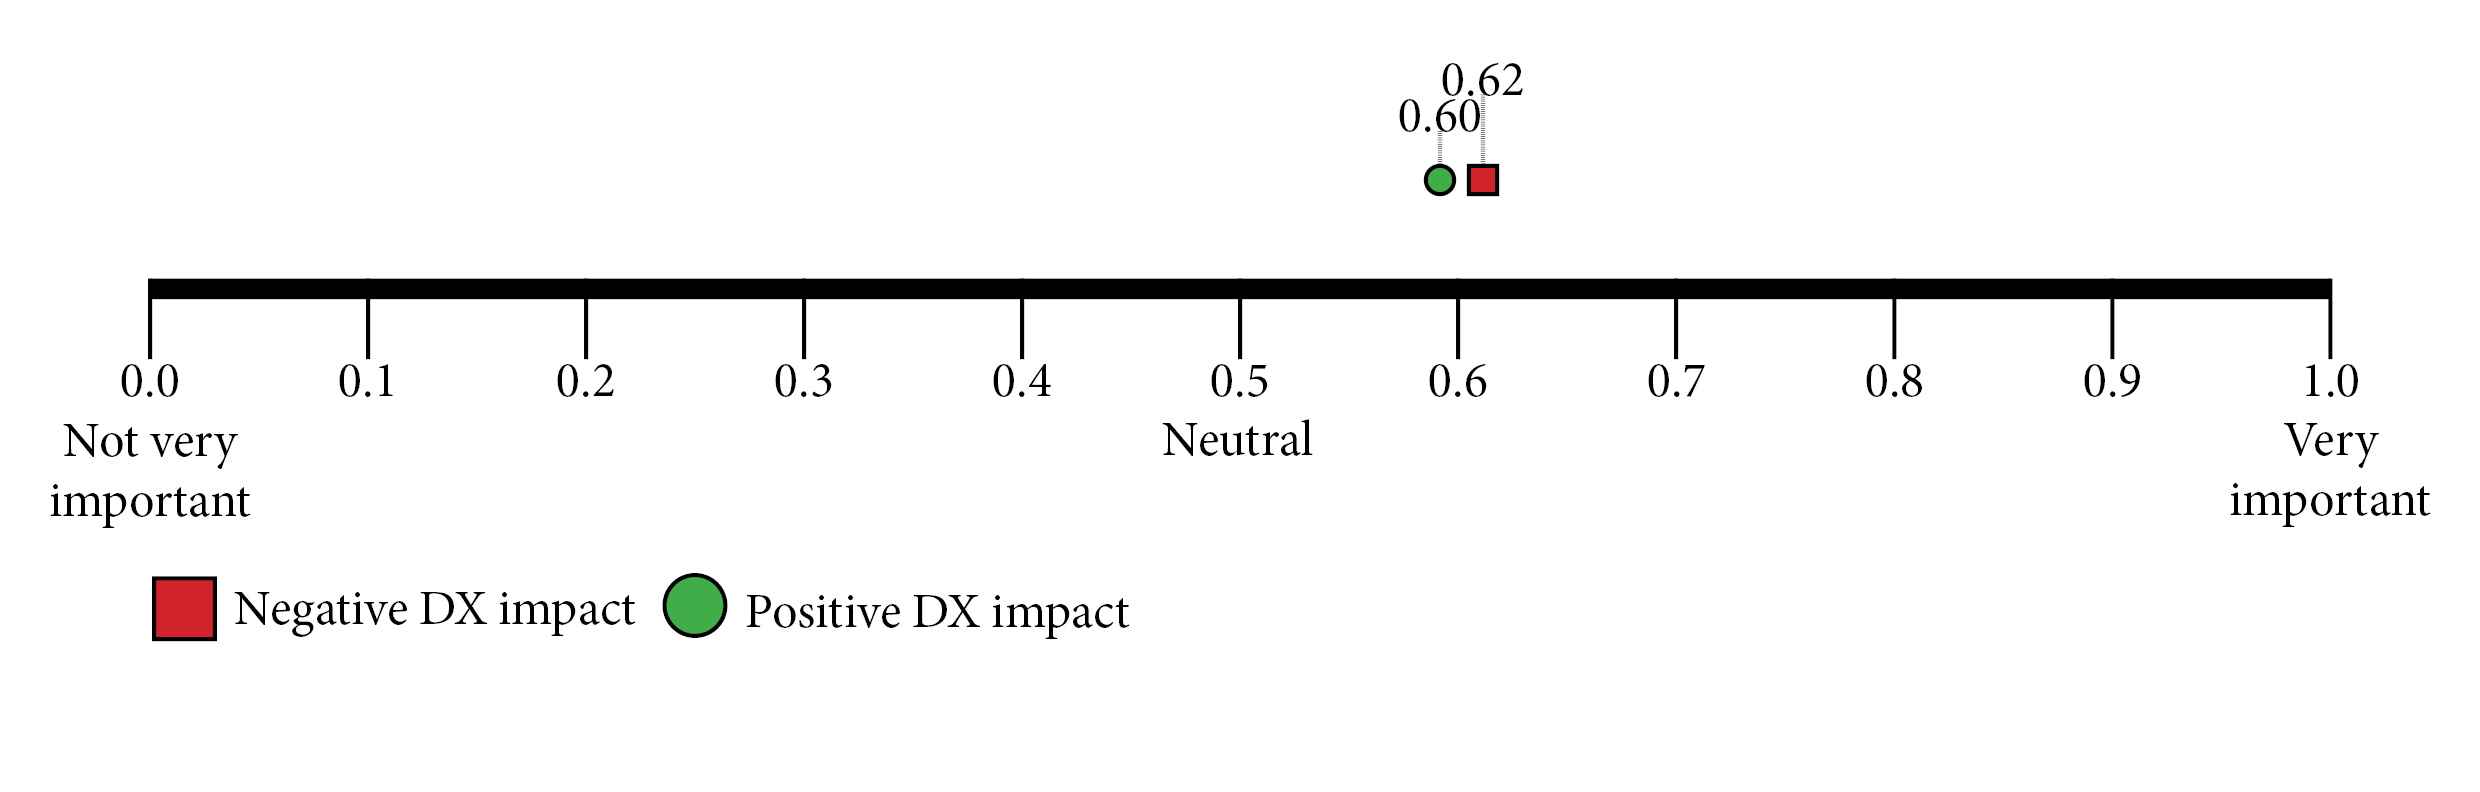
\includegraphics[width=\linewidth]{dxscorelines/dxaspect15.png}
\caption{Scoring for "The software uses the programming language I am most comfortable with"}
\label{fig:aspect15}
\end{figure}
Developers tend to be more comfortable working with certain languages, and it's unique for every person. As we can see in figure \ref{fig:aspect15} it is definitely something people consider. The DX impact shows however that they're not deterred by software platforms that is not in their favourite language. As stated before, providing several languages is not worth the effort. The recommendation is therefor to be attentive to what programming languages are popular, and to see how the trends change. Be aware however that these trends are just that, trends. New languages emerge all the time as "the new hot thing". The safer bet is to offer your software platform in a popular language, that is predicted to be popular for quite some time. \\ \\
\textbf{Verdict: Important. Medium effort, high payoff.}

\subsubsection{There exists an active online community around the software}
\begin{figure}[H]
\centering
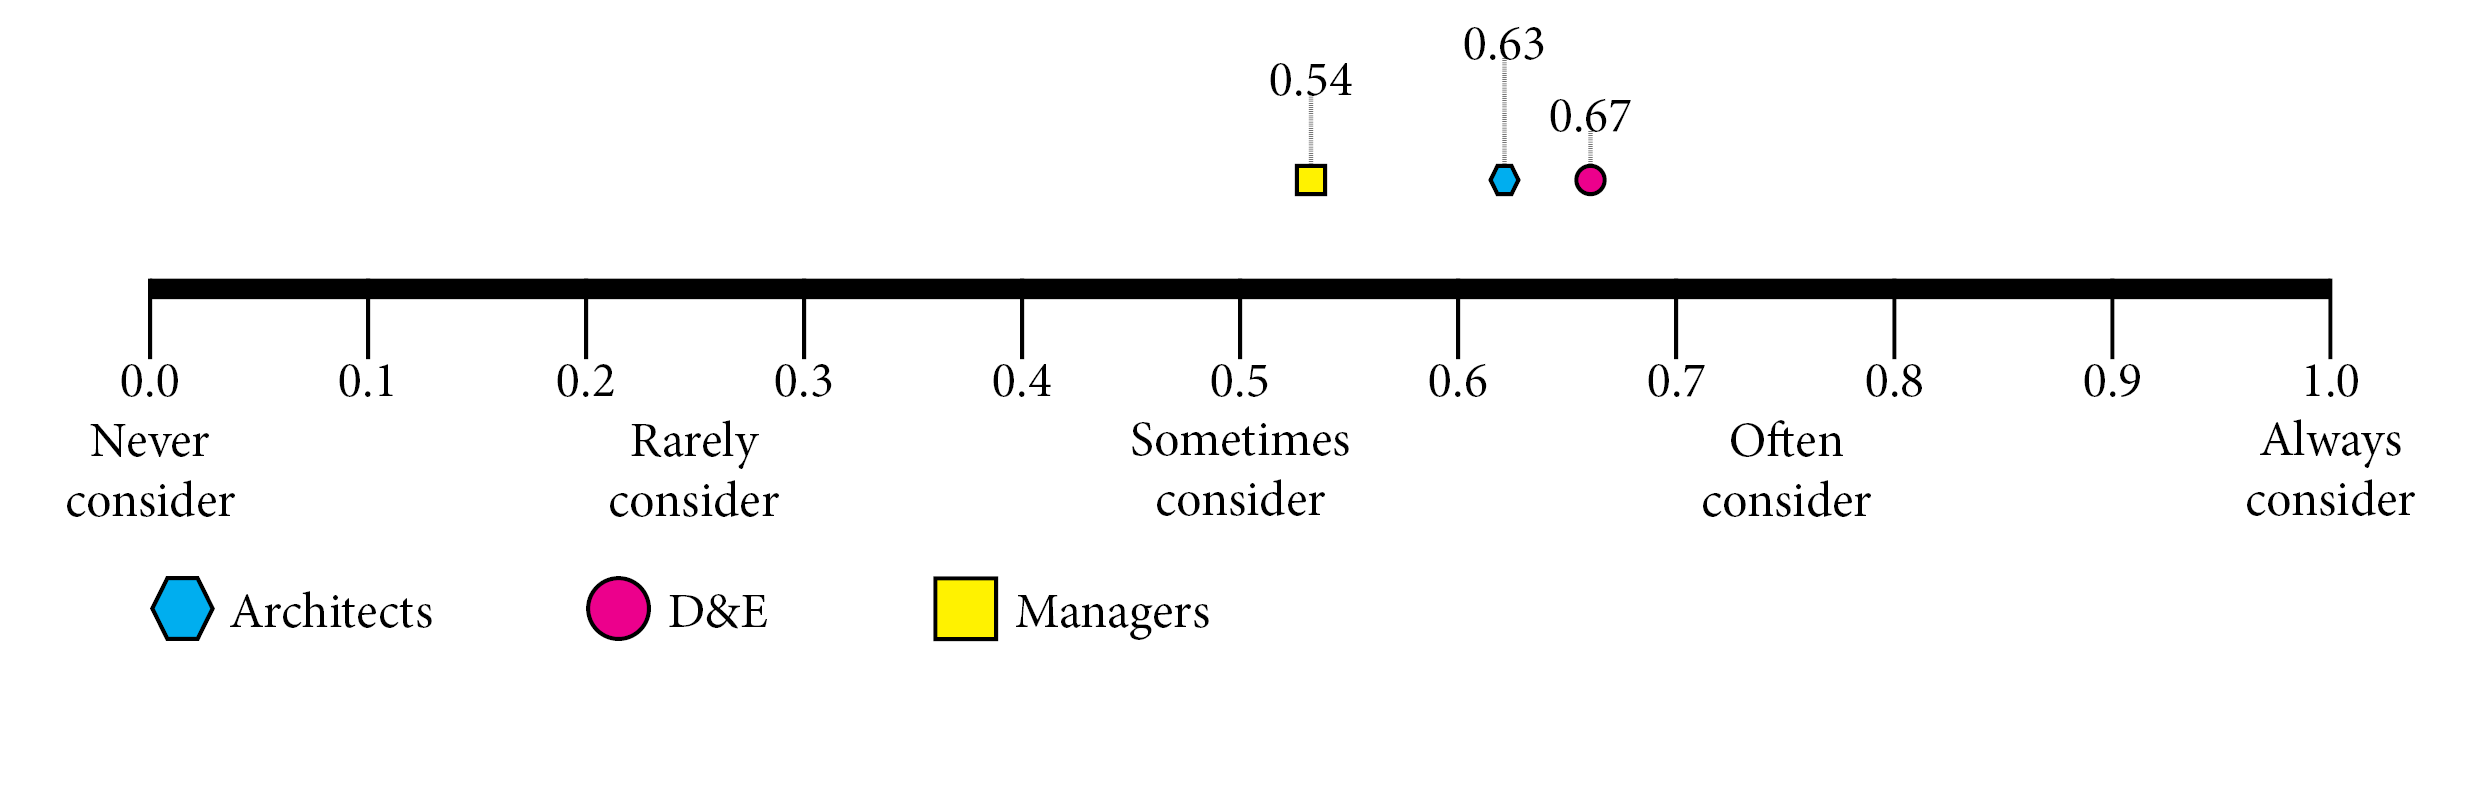
\includegraphics[width=\linewidth]{scorelines/aspect16.png}
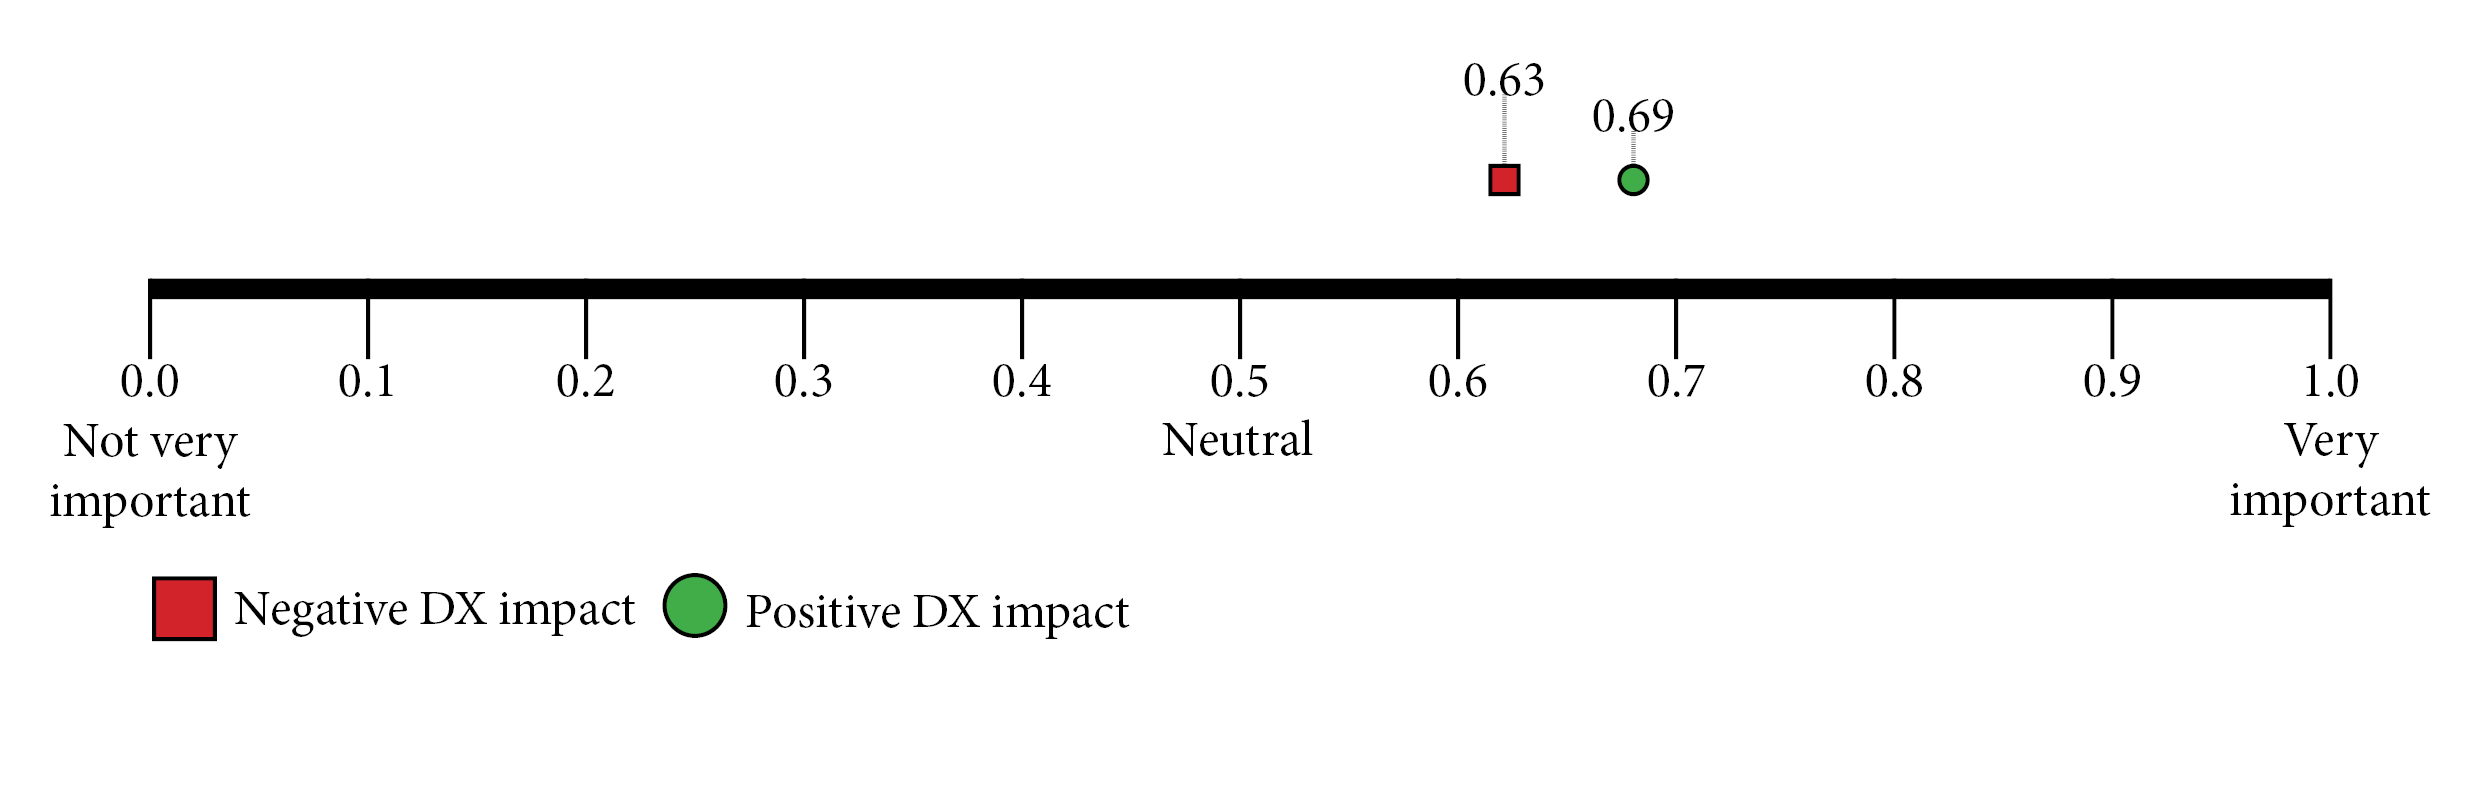
\includegraphics[width=\linewidth]{dxscorelines/dxaspect16.png}
\caption{Scoring for "There exists an active online community around the software"}
\label{fig:aspect16}
\end{figure}
It can be difficult, if not impossible, to forcefully create an online community around your software platform. It's not up to the company if people engage in online discussions, it's up to the users themselves. The company can however provide platforms for discussions. In figure \ref{fig:aspect16} we see that it's quite often considered, and a good community has above neutral DX impact on developers. 

The effort to create an online forum for users to discuss doesn't have to be too big, but acts as a starting point for a community to be created. Often communities will naturally emerge on other places, such as Stack Overflow. The company can help the online community prosper by keeping an eye on these communities as well, and answer question there. This also builds a trust between the user and the company.

Online communities is primarily used for questions and answers to help out when the documentation is not enough. The effort to make sure your online community has the answers they need is somewhat big. The recommendation is to take extra care of your online community when it's new and small, and less when it's big enough that it takes care of itself. Never ignore it though, pay attention to suggestions and issues that your online community has. \\ \\
\textbf{Verdict: Important, keep in mind. Medium effort, medium-high payoff.}
\subsection{Evaluation of Qlik Core}
\subsubsection{How often the software is updated}
Qlik Core is a quite new product, which left beta in mid-fall of 2018. At the date of writing this paper, they've made four updates since they left beta. They follow the recommendations, where they don't release too often, but clump them together into major releases.\\ \\
\textbf{Verdict: Pass}
\subsubsection{Having working code quickly}
When first visiting the website, my first instinct was to look for the phrases 'Try' or 'Getting Started'. You're greeted by a 'Try For Free', which I assumed was going to lead me to a page how I get started trying it out. That however lead me to a page about licensing. After that I saw the 'Get Started' in the top menu, which was what I was looking for initially. I afterwards realised that there was a button for 'Start Tutorials' on the start page, which leads the me to the same place as 'Getting Started'. I somehow missed this button. While this may be a one-off mistake by just me, it indicates that there's room for improvement. Rephrasing of these buttons may be in order. The start page can be seen in figure \ref{fig:startpage}. \\ \\
\begin{figure}[H]
    \centering
    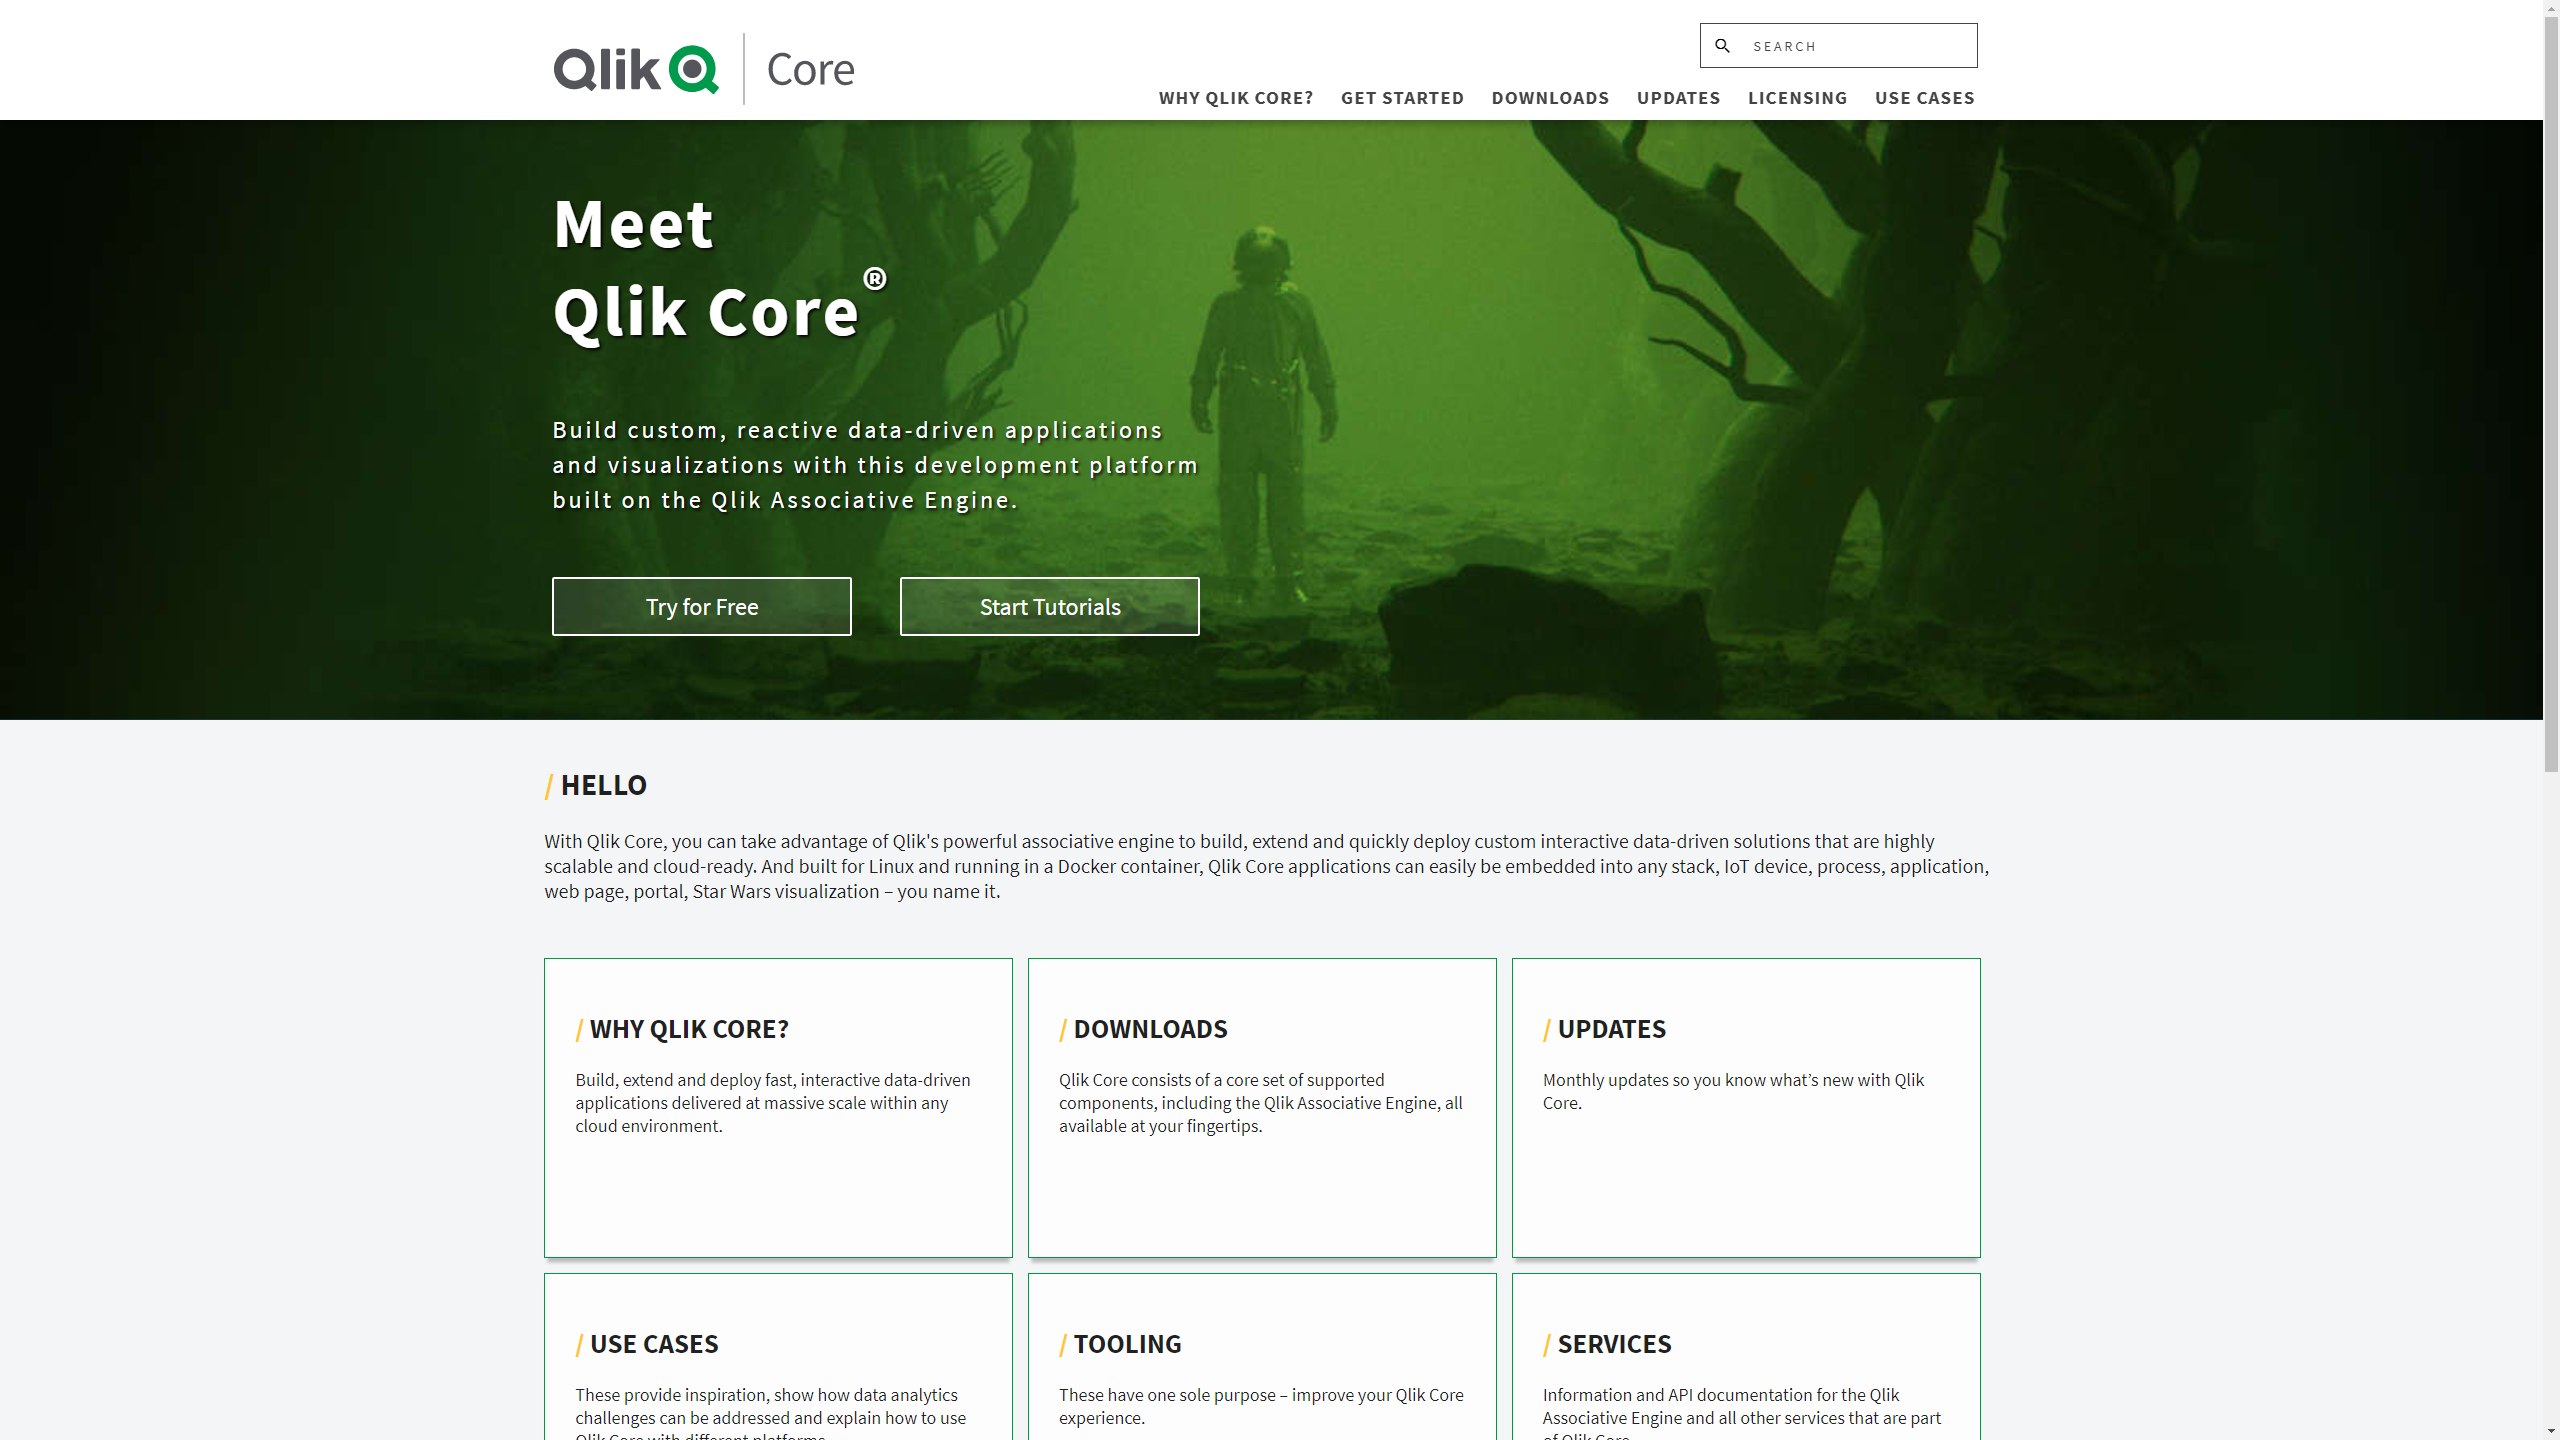
\includegraphics[width=\linewidth]{qlikCoreWebsite20190124.png}
    \caption{The Qlik Core start page on the 24\textsuperscript{th} January 2019}
    \label{fig:startpage}
\end{figure}
The 'Get Started' has a flow of text, where the actual tutorials are linked in the text flow. This requires the user who just wants to get started to read through the text. While this may be handy to put the user into context, when it comes to getting started quickly it slows the process down. Having these links be more in focus may speed up that process. The page can be seen in figure \ref{fig:gettingstarted}.
\begin{figure}[H]
    \centering
    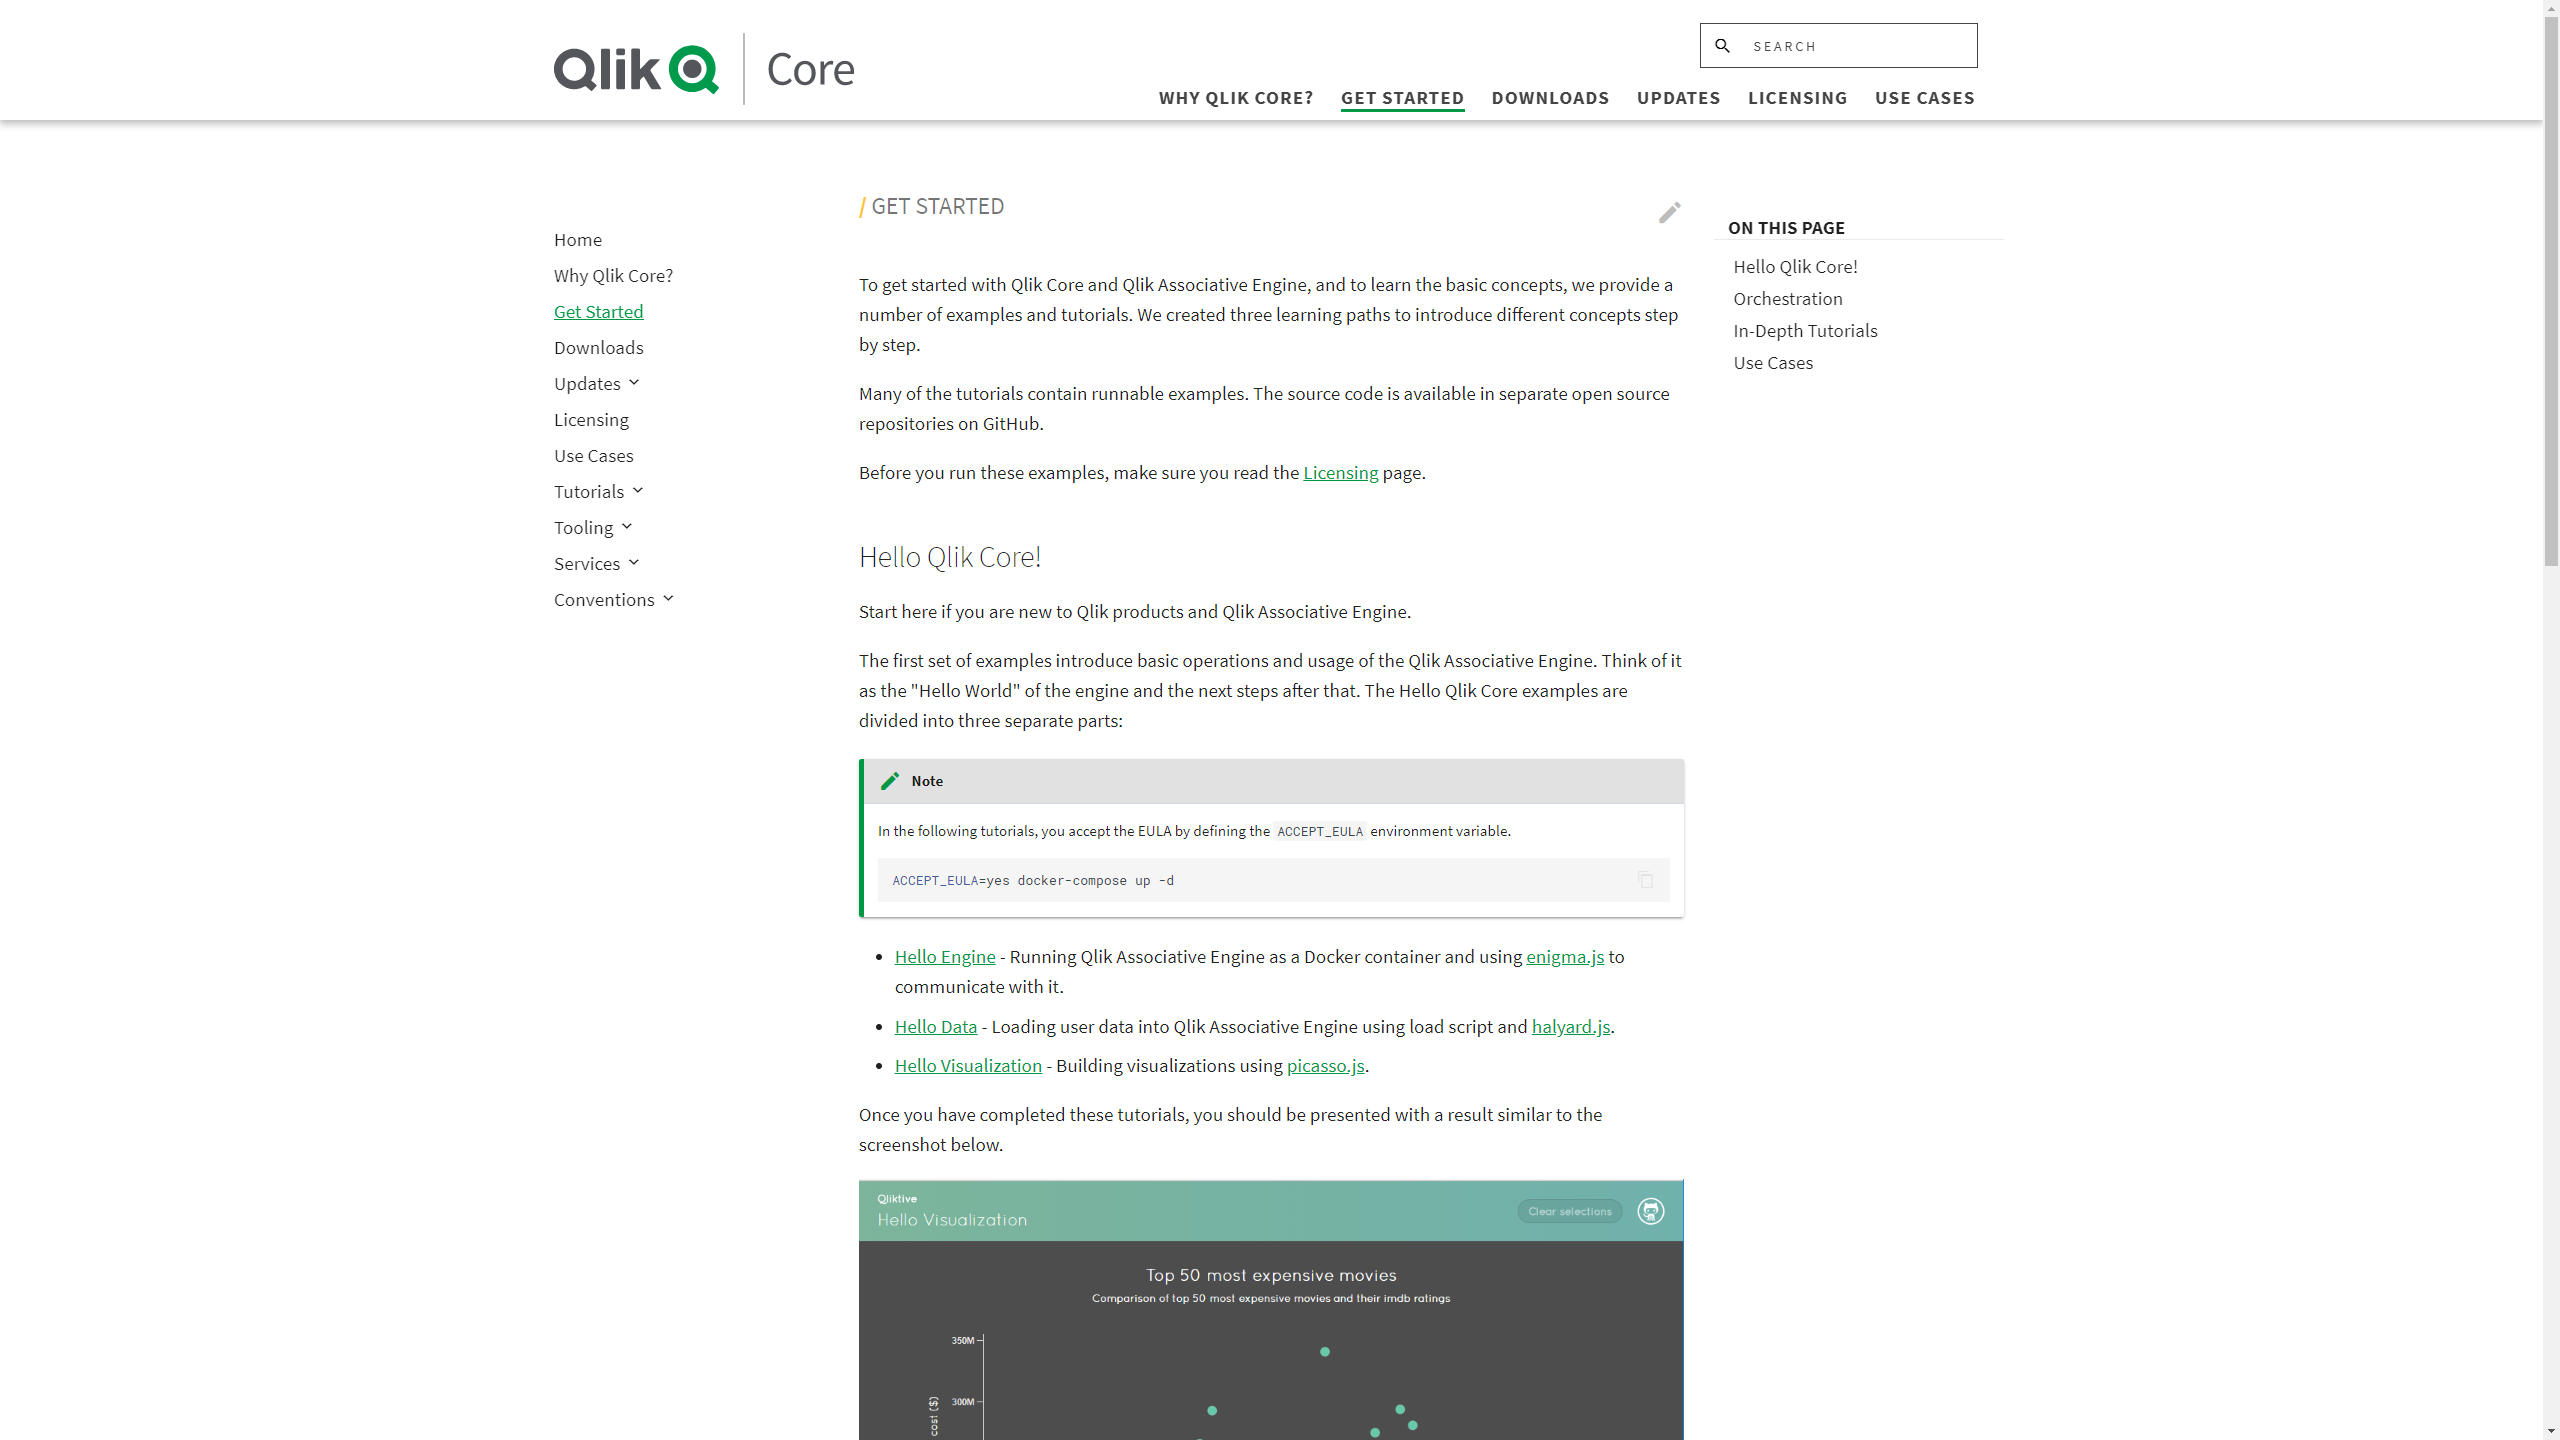
\includegraphics[width=\linewidth]{qlikCoreWebsite-GetStarted20190124.png}
    \caption{The Qlik Core Getting Started page on the 24\textsuperscript{th} January 2019}
    \label{fig:gettingstarted}
\end{figure}
Already one the first step I was at risk of being confused. They prompt you to run a command, but don't specify where. Clarifying that it should be in the newly cloned folder takes away that risk of confusion. The command failed with an error message that I did not help me. Here, I got stuck and had to ask for help from a coworker from the Qlik Core team. Turns out this was due to a lack of knowledge in how I should set up the third-party software they're relying on, Docker.\\ \\
The first tutorial called 'Hello-Engine' simply sets up the possibility to communicate with the engine. It was not clearly explained in the tutorial what the goal of the tutorial was, so when I finished I did not fully understand what I had finished. I thought that I had done something wrong, my thought was "This can't be it?" when I had actually completed the tutorial. Overall I had a lack of achievement, and did not feel I had learned anything about what Qlik Core is or can do. The following tutorial 'Hello Data' suffered a bit from the same issues. The third tutorial 'Hello Visualisation' was the first tutorial where I felt I had learned something about what Qlik Core can do. A tutorial should give the user a sense of achievement, and make the user feel like he or she learned something they did not previously know. In my opinion, these tutorials could be merged into one longer tutorial, divided into three sections. \\


The overall, getting started felt difficult. I was stopped by errors, getting a licence, setting up Docker configurations.
\section{Conclusion}
More text here...
\newpage
\bibliographystyle{unsrt}
\bibliography{references}
\end{document}
